%for a more compact document, add the option openany to avoid
%starting all chapters on odd numbered pages
\documentclass[12pt]{cmuthesis}

% This is a template for a CMU thesis.  It is 18 pages without any content :-)
% The source for this is pulled from a variety of sources and people.
% Here's a partial list of people who may or may have not contributed:
%
%        bnoble   = Brian Noble
%        caruana  = Rich Caruana
%        colohan  = Chris Colohan
%        jab      = Justin Boyan
%        josullvn = Joseph O'Sullivan
%        jrs      = Jonathan Shewchuk
%        kosak    = Corey Kosak
%        mjz      = Matt Zekauskas (mattz@cs)
%        pdinda   = Peter Dinda
%        pfr      = Patrick Riley
%        dkoes = David Koes (me)

% My main contribution is putting everything into a single class files and small
% template since I prefer this to some complicated sprawling directory tree with
% makefiles.

% some useful packages
\usepackage{tikz}
\usepackage{times}
\usepackage{fullpage}
\usepackage{graphicx}
\usepackage{amsmath}
\usepackage[numbers,sort]{natbib}
\usepackage{tabularx}
\usepackage{array}
\usepackage[table]{xcolor}
\usepackage{textcomp}
\usepackage{csquotes}
\usepackage{gensymb}
\usepackage[backref,pageanchor=true,plainpages=false, pdfpagelabels, bookmarks,bookmarksnumbered,
%pdfborder=0 0 0,  %removes outlines around hyper links in online display
]{hyperref}
\usepackage{subfig}

\usepackage{pifont}
\newcommand*\colourcheck[1]{%
        \expandafter\newcommand\csname #1check\endcsname{\textcolor{#1}{\ding{52}}}%
}
\newcommand*\colourcross[1]{%
        \expandafter\newcommand\csname #1cross\endcsname{\textcolor{#1}{\ding{53}}}%
}
\newcommand{\ooda}[0]{{\sc OODA}}
\newcommand{\norm}[1]{\left\lVert#1\right\rVert}
\colourcheck{green}
\colourcross{red}

% Approximately 1" margins, more space on binding side
%\usepackage[letterpaper,twoside,vscale=.8,hscale=.75,nomarginpar]{geometry}
%for general printing (not binding)
\usepackage[letterpaper,twoside,vscale=.8,hscale=.75,nomarginpar,hmarginratio=1:1]{geometry}

% Provides a draft mark at the top of the document. 
\draftstamp{\today}{DRAFT}

\begin {document} 
\frontmatter

%initialize page style, so contents come out right (see bot) -mjz
\pagestyle{empty}

\title{ %% {\it \huge Thesis Proposal}\\
{\bf Title Pending}}
\author{Mihir Bala}
\date{XX 2025}
\Year{2025}
\trnumber{}

\committee{
Mahadev Satyanarayanan, Chair \\
David O'Hallaron \\
Jeff Schneider \\
Padmanabhan Pillai
}

\support{}
\disclaimer{}

% copyright notice generated automatically from Year and author.
% permission added if \permission{} given.

\keywords{Autonomous Drones, Robotics, Mobile Computing, Edge Computing}

\maketitle

\begin{dedication}
TBD
\end{dedication}

\pagestyle{plain} % for toc, was empty

%% Obviously, it's probably a good idea to break the various sections of your thesis
%% into different files and input them into this file...

\begin{abstract}
To be written.
\end{abstract}

\begin{acknowledgments}
To be written.
\end{acknowledgments}



\tableofcontents
\listoffigures
\listoftables

\mainmatter

%% Double space document for easy review:
%\renewcommand{\baselinestretch}{1.66}\normalsize

% The other requirements Catherine has:
%
%  - avoid large margins.  She wants the thesis to use fewer pages, 
%    especially if it requires colour printing.
%
%  - The thesis should be formatted for double-sided printing.  This
%    means that all chapters, acknowledgements, table of contents, etc.
%    should start on odd numbered (right facing) pages.
%
%  - You need to use the department standard tech report title page.  I
%    have tried to ensure that the title page here conforms to this
%    standard.
%
%  - Use a nice serif font, such as Times Roman.  Sans serif looks bad.
%
% Other than that, just make it look good...

\chapter{Introduction}
\label{sec:introduction}
Unmanned aerial vehicles, commonly known as drones, are a disruptive technology that have recently seen widespread use. In civilian settings, they enable cheap and safe completion of tasks such as infrastructure inspection, agriculture monitoring, wildfire control, and police surveillance. In military settings, they are a vital tool for advance reconnaissance. For most use cases today, drones are deployed with a human pilot who is in constant control of the aircraft.

In recent years, research efforts have pushed towards drones capable of fully-autonomous flight. The term \textit{fully-autonomous} flight is defined by the National Institute of Science and Technology (NIST) as “pre-programmed flight without a remote human pilot, including mission-specific actions in response to runtime observations”~\cite{Huang2008}. There are two main benefits to this approach. First, it decreases costs and frees human attention. Second, it allows the practical operation of drone swarms, large groups of aircraft that cooperatively execute tasks. Drone swarms open the door to many missions that could revolutionize several civilian and military sectors~\cite{Burkle2009}. 

A key driver for fully-autonomous drones is the completion of active vision tasks~\cite{Aloimonos1988, Ognibene2013}. Active vision tasks require a drone to react in real time to its current scene interpretation. For instance, it may drop down to lower altitude without human intervention ``to take a closer look'' before the scene changes.  It may then return to its original altitude to continue monitoring the scene. This narrow scope of tasks characterizes many fundamental drone operations like following a target and evading obstacles.

Weight is a fundamental impediment to fully-autonomous drone adoption. Greater intelligence correlates with more powerful (and hence heavier) on-board computing and richer sensing. An on-board GPU, for example, brings with it a long logistical tail: heatsinks, cooling fans, and larger batteries. Increased weight brings with it regulatory challenges for flights over civilian areas. Since 2021, the FAA has pre-authorized flights over people and vehicles by drones with a total weight of less than 250~g~\cite{FAA2021}. Heavier drones require explicit FAA approval for such flights, conditional upon mitigation measures for collisions and free fall. Even above this limit, regulatory approval for autonomous BVLOS (beyond visual line of sight) flight in dense urban settings is easier to obtain for lighter drones than for heavier drones. This regulation has proven to be a major obstacle for several civilian projects. In military settings, weight is also a crucial consideration. Heavy aircraft complicate logistics and often require dedicated transportation~\cite{DefensePost}. 

Other major limitations to autonomous drone adoption are software portability, accessibility, mission versatility, and unit cost. While there have been attempts to bring all drones under a unified programming ecosystem, it is still the norm for drone companies to develop their own SDKs for their platforms. This makes it difficult to port code written for one ecosystem to another which divides the development community. Existing fully-autonomous drones also require users to have significant flight experience to ensure safe operation, a serious barrier to accessibility. Many lack versatility, and cannot be configured to perform missions outside of a small, manufacturer specified set. Lastly, the unit cost for current autonomous drones is several times higher than manually piloted equivalents. Such prices hurt the economic viability of swarm operations where individual aircraft losses are not only likely but expected.

The core contribution of this work is \textit{SteelEagle}, a hardware-agnostic autonomous drone system which attempts to surmount these obstacles by leveraging edge computing and a new modular drone operating system. Edge computing enables a drone to offload compute-intensive real-time operations over a low-latency, high-bandwidth wireless network to a powerful ground-based server (cloudlet) which is usually located near a cell tower. This reduces the need for heavy on-board computing hardware. In parallel, the SteelEagle operating system is designed to be drone agnostic, developer friendly, and mission centric.

A key consideration of this system is the use of commercial off-the-shelf~\cite{FAR} (COTS) drones and computing / communication payloads. This approach avoids customization of hardware (e.g., drone modifications) and modification of privileged software (e.g., “rooting” a device) which lowers cost and greatly increases accessibility. It also avoids the need for re-certification (e.g., by the FAA or the FCC). However, a COTS approach also introduces new obstacles. Thermal limitations of lightweight COTS communications devices pose latency, frame rate, and quality challenges, and force such systems to intelligently manage communication, computation, and prediction.

\section{Thesis Statement}
In this dissertation, I demonstrate SteelEagle as a capable alternative to existing autonomous drone systems, despite the inherent latency and bandwidth limitations of offloading. I show how it improves over other platforms in the following design categories:

\begin{enumerate}
\item \textbf{Weight}: the overall weight of the aircraft, including batteries and payload.
\item \textbf{Accessibility}: the barrier-for-entry to operate the aircraft. 
\item \textbf{Versatility}: the diversity of tasks which the system can execute.
\item \textbf{Portability}: the ease with which the system can be ported to new hardware.
\item \textbf{Cost}: the overall cost of the aircraft, including batteries and payload.
\end{enumerate}
\\
In particular, I claim that:
\newpage
\textbf{It is feasible to construct an ultra-light flight platform for autonomous active vision tasks in beyond visual line-of-sight (BVLOS) settings that only uses commercial off-the-shelf (COTS) drones and COTS computing/communication payloads. The most serious obstacle to this goal, namely the weight of computing hardware necessary to achieve autonomy, can be overcome using edge computing. I posit that such a flight platform can emulate the performance of heavier autonomous drones on active vision tasks, despite bandwidth, latency and connectivity challenges.}

\textit{Why is this thesis important?} If this statement were true, then such edge-enabled drones could see widespread adoption for BVLOS missions in urban environments. They would have lower operation costs and increased safety compared to traditional autonomous drones. Tasks such as structure inspection, police surveillance, and traffic monitoring could directly benefit from this. Drone swarms over public infrastructure would become safer.

\textit{Why does it not follow trivially from what is already known?} Existing work in this space is limited since most current research focuses on improving drone capabilities rather than decreasing their weight. There are no commercial drones under the FAA threshold of 250~g that possess onboard intelligence capable of autonomously executing  missions. There are limited drones that are edge-enabled, but these drones are heavy (more than 500~g) and expensive (over \$3,000). There has been some academic research on using drones in conjunction with edge computing, with full details provided in Section~\ref{sec:drone-and-the-edge}. However, these efforts focused on large, heavy drones which used onboard hardware in addition to supplemental edge offload. None identified weight as a dominant design consideration. SteelEagle, by contrast, is designed primarily around reducing weight without compromising capability. It is my belief that this is critical to drive large scale adoption of autonomous drones. 

\begin{flushleft}
The main contributions of this thesis are as follows:
\end{flushleft}
\begin{enumerate}
\item I describe a fully-autonomous flight platform capable of executing active vision tasks on lightweight COTS drones using edge computing. I show why this platform is an improvement over prior work in terms of its \textit{weight}, \textit{accessibility}, \textit{versatility}, \textit{portability}, and \textit{cost}.
\item I provide a measurement study quantifying this platform's performance using a novel benchmarking suite.
\item I show how this platform can be extended to a heterogeneous drone swarm ecosystem.  
\end{enumerate}

 

\section{Thesis Overview}
The remainder of this dissertation is organized as follows:
\begin{itemize}
    \item In Chapter 2, I provide background on the development history of autonomous drones and summarize related research in this area. I show how SteelEagle builds on this existing research.
    \item In Chapter 3, I discuss how to connect lightweight COTS drones to the edge. I outline the design challenges and formulate a criteria for choosing an edge communication payload that flies with the drone.
    \item In Chapter 4, I provide the overall design of SteelEagle including its advantages and disadvantages over current systems. I demonstrate a SteelEagle drone performing several autonomous tasks and provide some performance analysis.
    \item In Chapter 5, I introduce a new edge communication payload that improves on the earlier prototype. I show how this new payload can reduce the OODA (Observe Orient Decide Act) loop of the system, and thus greatly increase autonomous performance.
    \item In Chapter 6, I describe a family of benchmarks for measuring edge-based and fully-onboard autonomous drone performance on several key tasks. These benchmarks stress the OODA loop of the given test platform and are useful for understanding the impact of high latency and low throughput on edge offloading.
    \item In Chapter 7, I deploy SteelEagle on new drone hardware to demonstrate drone hardware agnosticism. I illustrate how my system adapts to different hardware and how it can cope with disconnected operation.
    \item Finally, in Chapter 8, I conclude the dissertation and explain future work with a summary of contributions.
\end{itemize}


\chapter{Background and Related Work}
Autonomous drones are an emerging field in both civilian and military sectors. The investment in Zipline, DJI, and other similar companies, show that there is a lucrative market for urban autonomous drone applications such as same-day drone delivery, automated infrastructure inspection, and programmable aerial surveillance~\cite{GrandviewResearchDroneMarket,ForbesZiplineEvaluation}. The rise of companies like Anduril and recent geopolitical events like the War in Ukraine also hint at the wider role that autonomous drones will play in future armed conflicts~\cite{CNBC,CFAS}.

Even with this demand, the quest to make smaller, lightweight autonomous drones is ongoing. Weight scales closely with the capability of onboard compute, and artificial intelligence algorithms used for drone perception continue to require more computation to run. This makes the prospect of creating a drone system with real-time access to such algorithms challenging.

In this chapter, I provide background on current autonomous drone platforms and outline how some of the obstacles impeding their practical deployment can be overcome. In Section \ref{sec:history-drone-development}, I briefly describe the history of drone development and regulation along with the different categories of modern drones. I also explain the various problems holding these systems back from widespread adoption. In Section \ref{sec:prior-work}, I discuss prior research that has attempted to solve these problems, and its limitations. In Section \ref{sec:better-autonomous-drones}, I propose a possible solution by leveraging the benefits of edge computing and COTS hardware. I show how the advantages of this approach could make autonomous drone deployment in urban environments a reality.

\section{The Development of Modern Drones}
\label{sec:history-drone-development}

Research into drone technology started in the early 1900s when during the interwar period, British engineers created a radio controlled plane, nicknamed the ``Queen Bee'', to train their anti-aircraft gunnery~\cite{IWMDrone}. The Queen Bee's name would spawn the colloquial ``drone'' moniker when referring to radio-controlled aircraft, a reference to worker drones in bee colonies. Over the next several decades, militaries around the world began incorporating drones into their arsenals; first, as pilotless training targets but later, as remotely operated observation and strike aircraft. By the 1990s, drones had become very sophisticated, equipped with multiple onboard sensors which enabled these platforms to conduct aerial reconnaissance at great distances~\cite{GlobalHawk}. However, despite these advances, one core design tenet remained unchanged: drones were always controlled by a human pilot and had limited ability to function on their own.

\begin{figure}%
    \centering
    \subfloat[\centering The British-made "Queen Bee", introduced in 1935, was one of the first radio operated aircraft and served as an anti-aircraft practice target~\cite{IWMDrone}.]{{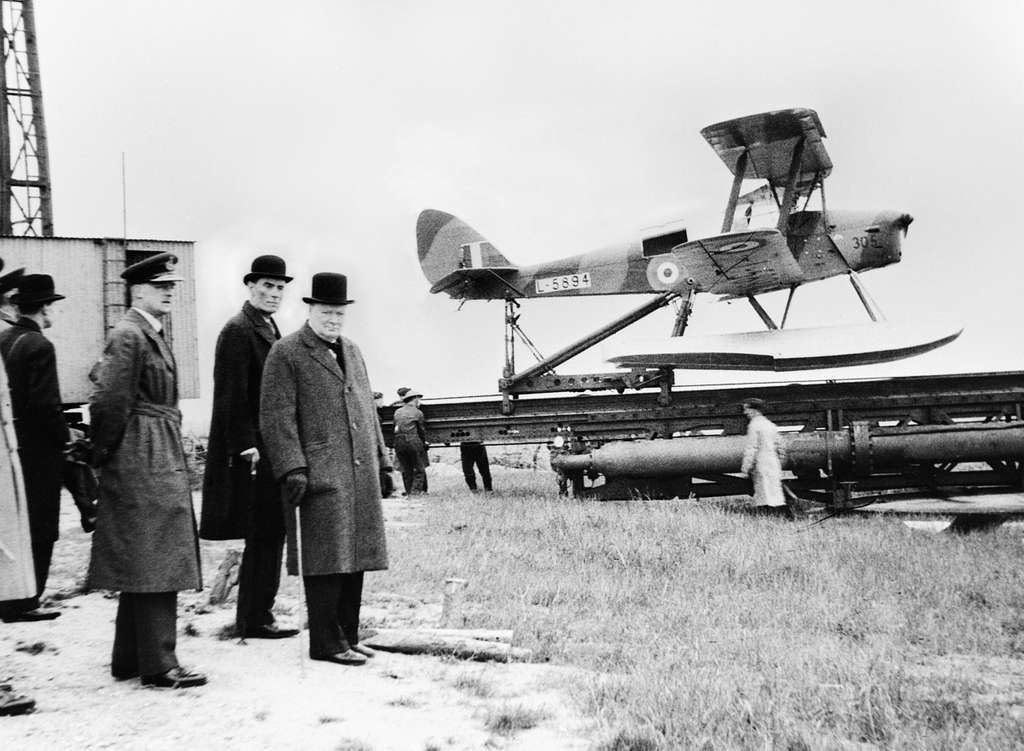
\includegraphics[width=7cm, height=5cm]{chapter2/FIGS/qbee2.jpg}}}%
    \qquad
\subfloat[\centering The RQ-4 Global Hawk, introduced in 1998, is a currently operated US Air Force reconnaissance drone with a range of over 14,000 miles~\cite{GlobalHawk}.]{{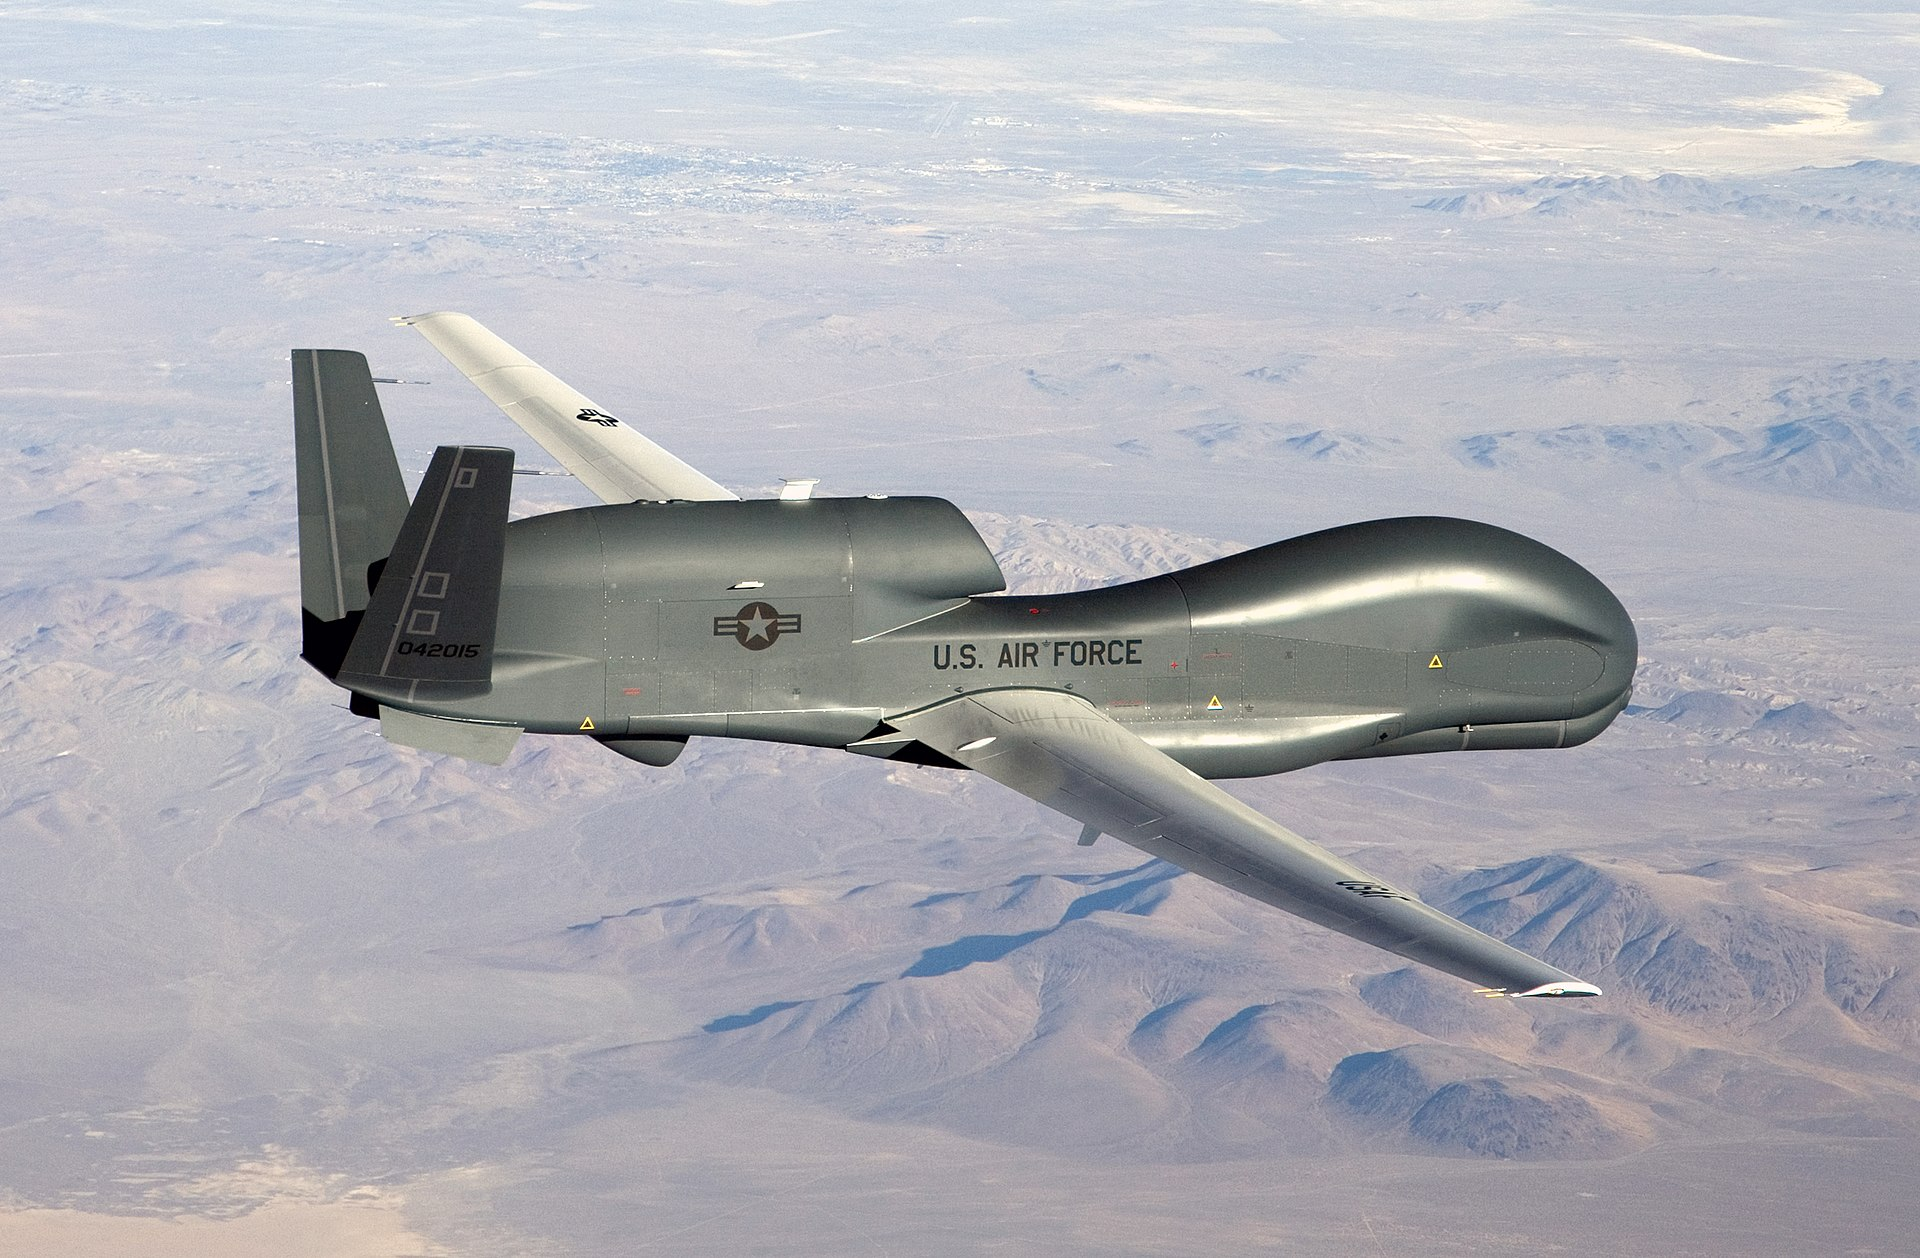
\includegraphics[width=7cm, height=5cm]{chapter2/FIGS/globalhawkdrone.jpg} }}%

    \subfloat[\centering The Skydio 2, released in 2019, provides a small set of semi- and fully-autonomous capabilities like person tracking and obstacle avoidance~\cite{Skydio2}.]{{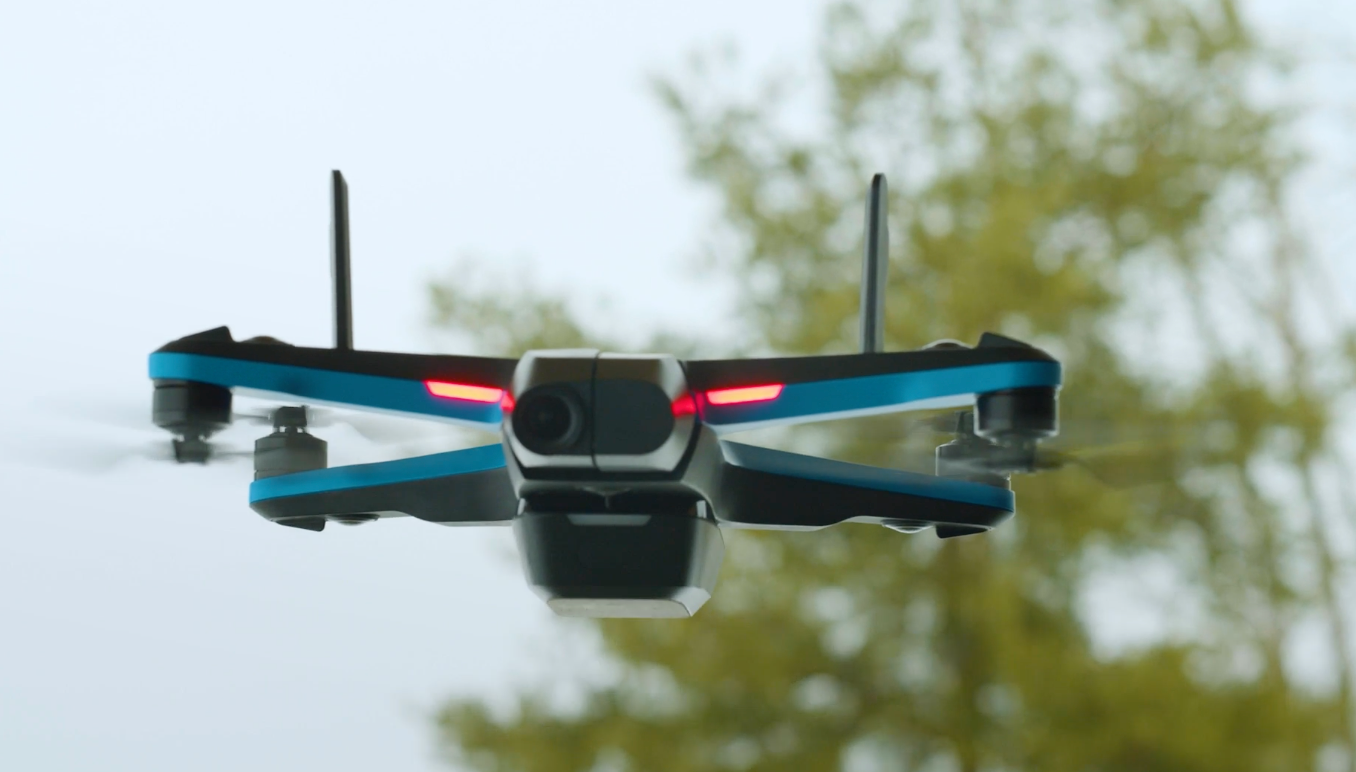
\includegraphics[width=7cm, height=5cm]{chapter2/FIGS/skydio-2.png} }}%
    \qquad
    \subfloat[\centering The DJI Matrice 600, released in 2016, is a fully-programmable autonomous drone with support for native onboard GPUs. Its huge size limits practical deployment~\cite{DJIMatrice}.]{{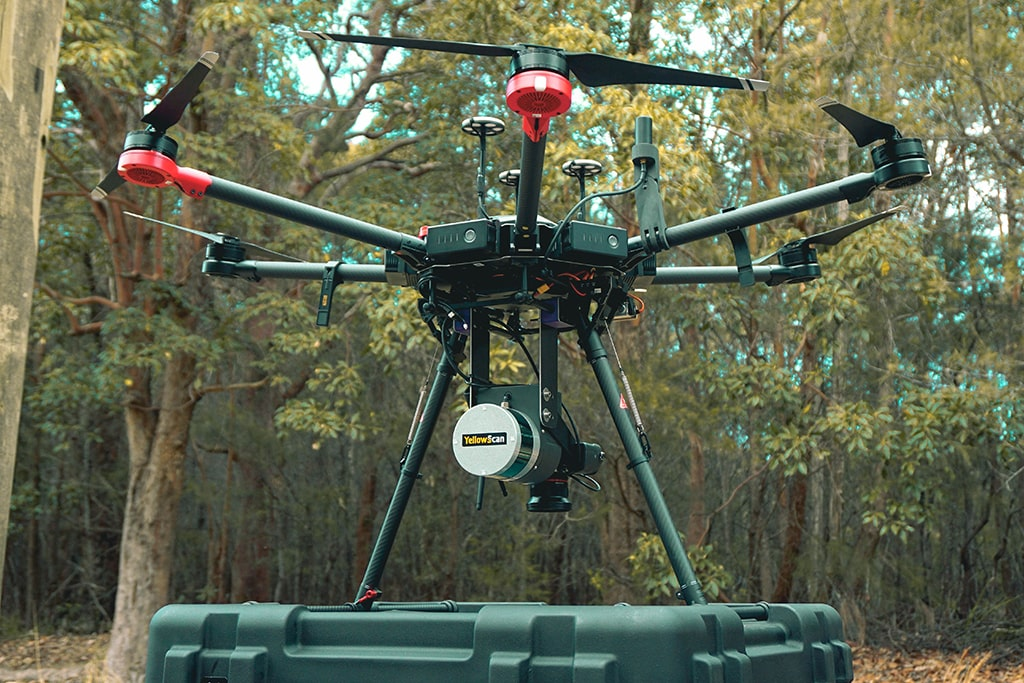
\includegraphics[width=7cm, height=5cm]{chapter2/FIGS/matrice600-2.png} }}%
    \caption{Evolution of Drone Technology}%
    \label{fig:20th-century-drones}%
\end{figure}

In the mid 2010s, drone technology started to shift away from exclusive manual piloting. The release of commercial autopilots like Pixhawk4 and Ardupilot enabled the rise of miniaturized (under 2~kg) multirotor drones which could perform limited autonomous flight such as following preset GPS waypoints~\cite{Pixhawk,Ardupilot}. Later, this was extended to semi-autonomous visual tracking and autonomous obstacle avoidance in quadrotor offerings like the DJI Phantom 4 and the Skydio 2~\cite{DJIPhantom4,Skydio2}. At the same time, growing investment in commercial fully-autonomous drones yielded the first off-the-shelf products. The DJI Matrice series (around 1~kg) was the most prominent of these, and it offered fully-autonomous capabilities using an onboard embedded computer, the DJI Manifold~\cite{DJIMatrice}.

While the drone space is diverse in both aircraft size and type, this thesis will focus on quadrotor drones. Quadrotors are by far the most common drone type and have a number of advantages over fixed-wings and helicopters. Namely, they are affordable, easy to use, and are very stable in flight. These make them perfect for tasks involving aerial imagery analysis which are the main focus of this thesis. For the rest of this document, all mention of ``drones'' will refer to quadrotor aircraft.

\begin{figure}
    \centering
    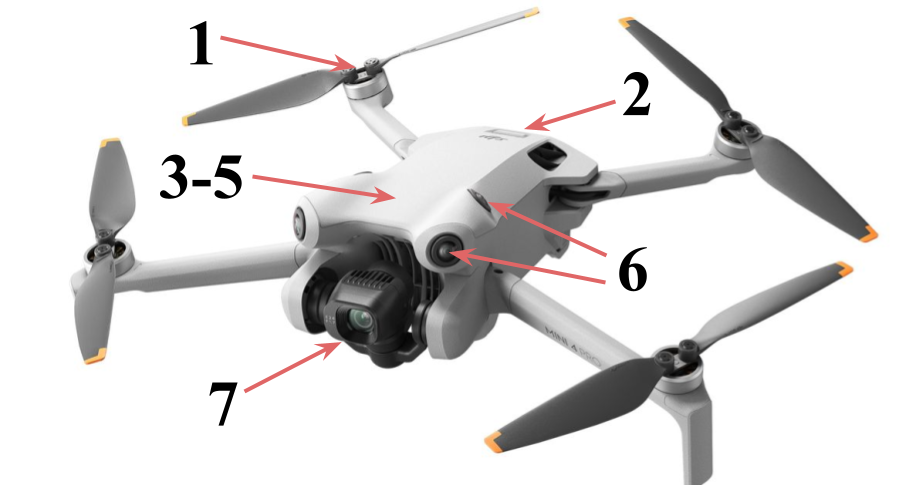
\includegraphics[width=0.75\linewidth]{chapter2/FIGS/anatomy.png}
    \begin{captext}
    \small \\ The main components of a modern consumer drone: \\\textit{\textbf{1.} rotors, \textbf{2.} hot-swappable battery, \textbf{3.} autopilot, \textbf{4.} sensor module, \\ \textbf{5.} companion computer, \textbf{6.} stereo cameras, \textbf{7.} gimbal camera.}
    \end{captext}
    \caption{Quadrotor Drone Anatomy}
    \label{fig:drone-anatomy}
\end{figure}

\subsection{Anatomy of a Drone}
Modern quadrotor drones are made up of several key components. Broadly, these accomplish one of four tasks: \textit{low-level flight control, high-level flight control, power, and sensing}. Figure~\ref{fig:drone-anatomy} uses the DJI Mini 4 Pro~\cite{DJIMini4}, a popular consumer drone, to illustrate these components:

\begin{enumerate}
    \item \textbf{Rotors} (low-level flight control): provide lift to the aircraft. Opposing pairs counter-rotate to provide stability~\cite{Allain2017}. Rotors are coordinated by the electronic speed controller (ESC), a micro-controller connected to the \textit{Autopilot} module~\cite{Nagel2023}.
    \item \textbf{Battery} (power): delivers power to all components. In many consumer drones, like the DJI Mini 4 Pro, the battery is a separate part which can be easily swapped out in the field.
    \item \textbf{Autopilot} (low-level flight control): works with the ESC to execute flight maneuvers. Uses telemetry from the \textit{Sensor Module} to compensate against the wind and maintain a stable hovering position. Acts as a software abstraction layer over all drone sensors and hardware. Also manages the radio connection to the pilot.
    \item \textbf{Sensor Module} (sensing): provides information about the drone's position and orientation, also known as telemetry. Usually made up of a GPS antenna, an inertial measurement unit (IMU)~\cite{IMU}, an altimeter, and a compass.
    \item \textbf{Companion Computer} (high-level flight control): responsible for high-level autonomous decision-making. Runs computer vision or sensor fusion algorithms then sends actuation commands to the \textit{Autopilot} based on the outputs.
    \item \textbf{Stereo Cameras} (sensing): gives a real-time depth map of the drone's surroundings~\cite{Stereo}. This enables full 360-degree obstacle avoidance. Not a feature on all consumer drones but becoming increasingly common.
    \item \textbf{Gimbal Camera} (sensing): the main camera through which the drone visually senses its surroundings. Able to pitch, yaw, or roll as commanded by the \textit{Autopilot}.
\end{enumerate}
In some cases, drones may be equipped with special equipment like LIDAR, time-of-flight sensors, RTK modules, and cellular modems. However, these are rare and are usually a feature of purpose-built aircraft for specific mission sets. 

\begin{figure}
    \centering
    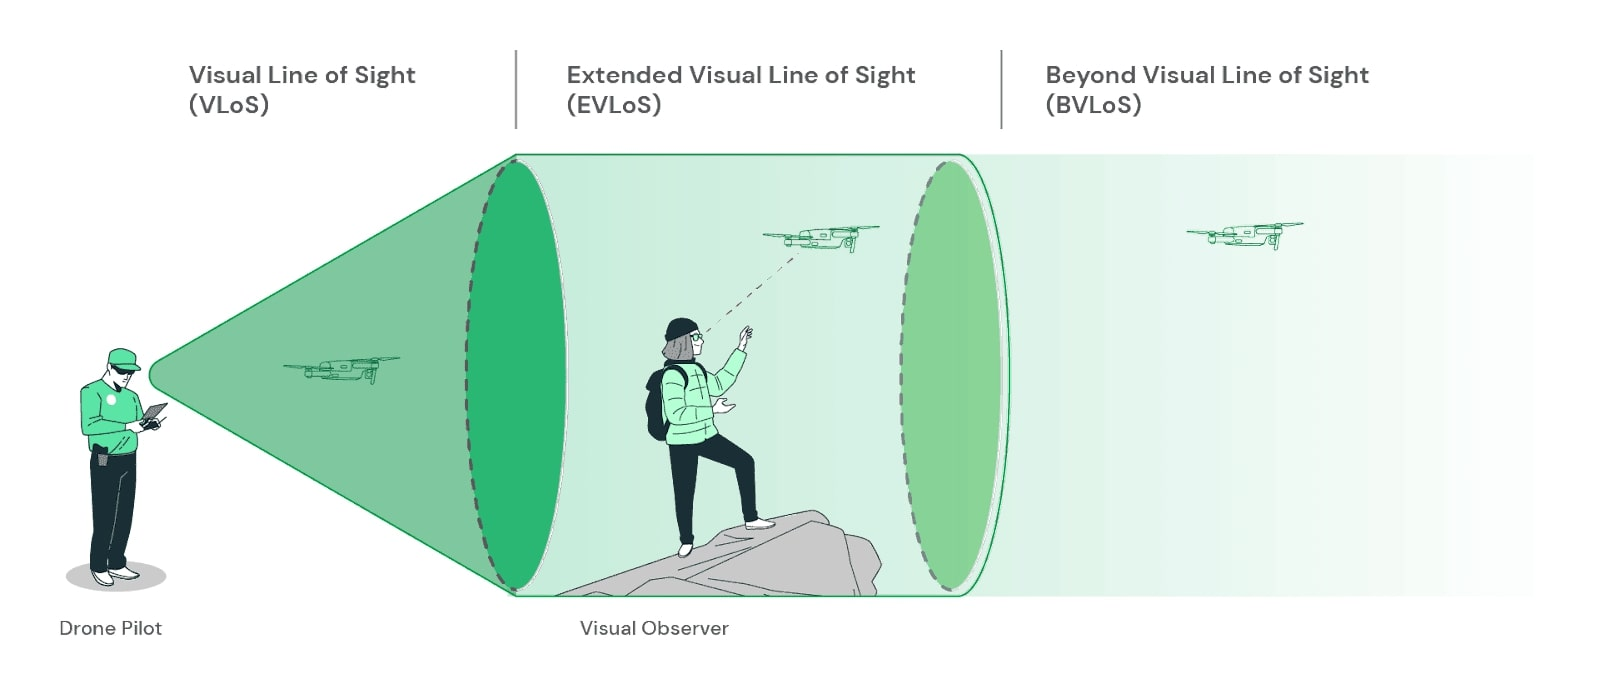
\includegraphics[width=1.0\linewidth]{chapter2/FIGS/bvlos.jpg}
    \caption{Types of Line-of-Sight Operation}
    \label{fig:bvlos}
\end{figure}

\subsection{Regulation in Civilian Airspace}
Drones like the DJI Mini 4 Pro and others are available globally for purchase, generally without the need for a license. This has led to a rapid dissemination of drones to consumers across the world and has spurred government regulators into action. This regulation serves one major purpose: to prevent potential damage to people or property due to in-flight emergencies. In the United States, the Federal Aviation Administration (FAA) introduced the Part 107 regulation in 2016~\cite{Flexairco}. This explicitly outlined the classes of UAVs allowed to fly over people, citing that only aircraft under 0.55~lbs or 250~g enjoyed near-unconditional approval~\cite{FAA2021}. In Europe, the European Union Aviation Safety Agency (EASA) has introduced similar regulation, only permitting flights over uninvolved pedestrians for drones under 250~g~\cite{EASA}. Flights over assemblies of people are not allowed for any weight class. In other countries, drones under 250~g are not regulated at all~\cite{IndiaRegulation,ChinaRegulation}.

In addition to weight regulation for flights over people, most countries also have restrictions on beyond visual line-of-sight (BVLOS) operation of heavy drones. BVLOS operation is defined as flying outside the visual range of the pilot (referred to as the RPIC, or remote pilot-in-command by the FAA) and outside the visual range of an observer within radio contact with the RPIC~\cite{BVLOS}. Figure~\ref{fig:bvlos} shows the different classes of line-of-sight operations.

\subsection{The Current Drone Market}
\label{sec:current-market}
As a result of both regulation and consumer demand, the current drone market is segmented into three loose categories: fully-autonomous, semi-autonomous, and manually piloted drones. Each of these inhabits a different weight and mission class, and are designed to operate in different regulatory environments. Table~\ref{tab:drone-apps} exhibits the main applications that drones are designed for. Generally, depending on regulation in the mission area, either a semi-autonomous (heavily-regulated) or fully-autonomous (lightly-regulated) drone will be used. 

\begin{enumerate}
    \item \textbf{Manually-Piloted Drones}: Manually-piloted drones are designed for hobbyist consumers, usually for the purpose of drone racing or recreational RC flight. They have no onboard compute, are not programmable, and must be manually piloted at all times to function. An example of a manually-piloted drone is the iFlight Cidora. This class of drone is extremely lightweight and very affordable compared to both semi- and fully-autonomous drones. The iFlight Cidora weighs 115~g and costs \$295 per unit~\cite{Cidora}. Most manually-piloted drones are so light that they avoid regulation.
    \\
    \item \textbf{Semi-Autonomous Drones}: Semi-autonomous drones have limited onboard compute and cannot perform active vision tasks without a human in the loop. They are typically equipped with a commercial autopilot like Pixhawk4 which enables autonomous following of GPS waypoints and automatic stabilization. They are not intended to operate BVLOS and often require a constant link to the RPIC (remote pilot in command). An example of a semi-autonomous drone is the Parrot Anafi. It is programmable and has no onboard compute, but can follow GPS waypoints and perform limited visual tracking by offloading to the RPIC's controller. This class of drone is lightweight and affordable compared to fully-autonomous drones, and can usually be flown in dense urban environments with minimal regulatory hurdles. The Parrot Anafi weighs 320~g and costs \$470 per unit~\cite{ParrotAnafi}.
    \\
    \item \textbf{Fully-Autonomous Drones}: Fully-autonomous drones have significant compute resources onboard and are able to analyze their own sensor streams in real time. They can perform active vision tasks without human assistance and can operate BVLOS. They also are fully-programmable, often outfitted with an onboard computer and flight control API. An example of a fully-autonomous drone is the DJI Matrice series. This class of drone is typically heavy and expensive. The Matrice 300 RTK, for instance, is over 3.5~kg and over \$10,000 per unit~\cite{Matrice300RTK}. Because of their size and weight, fully-autonomous drones are generally limited to use in rural areas away from people or property.
    \\
\end{enumerate}
In reality, most drones share traits from all three of these categories, and seldom fit into one cleanly. This motivates viewing the drone space as a ``spectrum of autonomy'', from least (manually-piloted) to most (fully-autonomous). Figure~\ref{fig:spectrum} shows the capabilities of several popular drones and where they would lie on this theoretical spectrum.


\begin{table}
    \centering
    \rowcolors{2}{gray!10}{white}
    \begin{tabularx}{\textwidth}{| m{2.8cm} | m{12.5cm} |}
        \hline
        \centering \makecell{Precision\\Agriculture} & 
        \small Drones are very useful for precision agriculture, with uses in monitoring, planting, irrigation, and pollination. They are easily scalable for large crop fields and can cover more area than ground-based solutions~\cite{Croptracker}. Most drone agriculture solutions use heavy, fully-autonomous platforms since rural areas have less strict regulation. \\[0.1cm]
        \hline
        \centering\makecell{Search and\\Rescue} & 
        \small Aerial vehicles have historically been a vital component in search and rescue. Drones fit nicely into this role, allowing search and rescue teams to scan an area at a much lower altitude than they could with traditional aircraft. They have seen real world use in the wake of the 2010 Haiti earthquake and other natural disasters~\cite{SARDrone}. \\[0.1cm]
        \hline
        \centering\makecell{Package\\Delivery} &
        \small For many years, drones have been touted as the future of last mile package delivery. This is because they can operate with higher cost-efficiency for small size items and can reach areas that are not well-connected by traditional infrastructure~\cite{PackageDrone}. Amazon has invested heavily in Prime Air, a drone-based extension to its popular Prime delivery service. However, this project has been sidelined by FAA regulation~\cite{Link2023}. Other companies like Zipline have had more success, using drones to make 1 million deliveries to remote areas~\cite{ForbesZiplineDeliveries}. \\[0.1cm]
        \hline
        \centering\makecell{Structure\\Inspection} &
        \small Recently, drones have emerged as a useful tool for structure inspection. They are able to reach inaccessible sections of structures due to their small size and maneuverability. More importantly, they are much safer and efficient than a human inspector. In 2022, the U.S. Bureau of Labor Statistics estimated that 1 in every 5 construction workplace deaths was due to falls~\cite{ConstructionFalls}. Drones allow pilots to view unsafe areas with no personal risk. This has increased the frequency of building inspection checkups, ensuring prompt, safe maintenance on failing infrastructure~\cite{InfrastructureInspection}. \\[0.1cm]
        \hline
        \centering\makecell{Aerial\\Surveys} &
        \small While aerial surveys and 3D scans have been conducted for decades, drones are a new, more cost effective tool for this task~\cite{AerialPhotography}. Their ability to provide a high resolution, bird's eye view of an area combined with their flight stability, make them ideal candidates for survey work. \\[0.1cm]
        \hline
        \centering\makecell{Police\\Work} &
        \small Drones have seen an increasing role in law enforcement. Agencies use them for general surveillance, illegal activity monitoring, crime scene investigation, and many other mission sets~\cite{PoliceDrone}. Companies like Skydio and DJI focus many offerings on this market segment. \\[0.1cm]
        \hline
        \centering\makecell{Aerial\\Reconnaissance} &
        \small Modern drones have revolutionized military aerial reconnaissance. Their small size allows them to be carried with a squad and deployed on-the-fly when necessary~\cite{StarsStripes}. The U.S. military has also invested in micro-scale platforms like the Teledyne Black Hornet that could conceivably be carried by every soldier~\cite{StarsStripes}. \\[0.1cm]
        \hline
        \centering\makecell{Suicide\\Aircraft} & 
        \small Suicide drones have been one of the most impactful new weapons in the War in Ukraine. Both Russian and Ukrainian forces have used small quadcopters like the DJI Mavic 3 to deliver bomb payloads~\cite{BBCKamikaze}. These have been very effective against slow moving targets like tanks~\cite{FPKamikaze}. Some fear that this technology could lead to a new breed of terrorist attacks~\cite{Pledger2021}. \\[0.1cm]
        \hline
        \centering\makecell{Anti-Drone\\Defense} &
        \small As the threat of drones has increased, the investment in drone defense systems has surged. Companies like Anduril have tackled this problem by using specialized drones to take down other hostile drones. Their Anvil kinetic interceptor destroys other UAVs by smashing into them at high speeds~\cite{Anvil}. \\[0.1cm]
        \hline
    \end{tabularx}
    \caption{Drone Applications}
    \label{tab:drone-apps}
\end{table}

\begin{figure}[]
    \centering
    \begin{tabular}{|c|c|c|c|c|c|}
        \hline
           \rowcolor{lightgray!50}
         \textbf{Drone} & \textbf{Autopilot} & \textbf{Avoidance} & \textbf{Tracking} & \textbf{Programmable} & \textbf{Compute} \\
         \hline
         iFlight Cidora & \cellcolor{green!20}None & \cellcolor{green!20}None & \cellcolor{green!20}None & \cellcolor{green!20}No & \cellcolor{green!20}None \\[0.1cm]
         \hline
         DJI Avata 2 & \cellcolor{orange!25}Yes & \cellcolor{yellow!20}Partial & \cellcolor{green!20}None & \cellcolor{green!20}No & \cellcolor{green!20}None \\[0.1cm]
         \hline
         Parrot Anafi & \cellcolor{orange!25}Yes & \cellcolor{green!20}None & \cellcolor{yellow!20}Assisted & \cellcolor{red!20}Yes & \cellcolor{green!20}None \\[0.1cm]
         \hline
         Skydio 2 & \cellcolor{orange!25}Yes & \cellcolor{orange!25}Yes & \cellcolor{yellow!20}Assisted & \cellcolor{yellow!20}Partially & \cellcolor{green!20}None \\[0.1cm]
         \hline
         DJI Mini 4 Pro & \cellcolor{orange!25}Yes & \cellcolor{orange!25}Yes & \cellcolor{yellow!20}Assisted & \cellcolor{yellow!20}Partially & \cellcolor{green!20}None \\[0.1cm]
         \hline
         Skydio 2 & \cellcolor{orange!25}Yes & \cellcolor{orange!25}Yes & \cellcolor{red!20}Yes & \cellcolor{yellow!20}Partially & \cellcolor{red!20}Yes \\[0.1cm]
         \hline
         DJI Matrice 300 RTK & \cellcolor{orange!25}Yes & \cellcolor{orange!25}Yes & \cellcolor{red!20}Yes & \cellcolor{red!20}Yes & \cellcolor{red!20}Yes \\[0.1cm]
         \hline
    \end{tabular}
    \\[0.2cm]
    \begin{captext}
        \small Capabilities are colored according to whether they are typically associated with manually-piloted (green), semi-autonomous (yellow), both semi- and fully-autonomous (orange),  or fully-autonomous (red) drones. Assisted tracking means that a human pilot must help the drone in order for it to function properly.
    \end{captext}
    \centering
    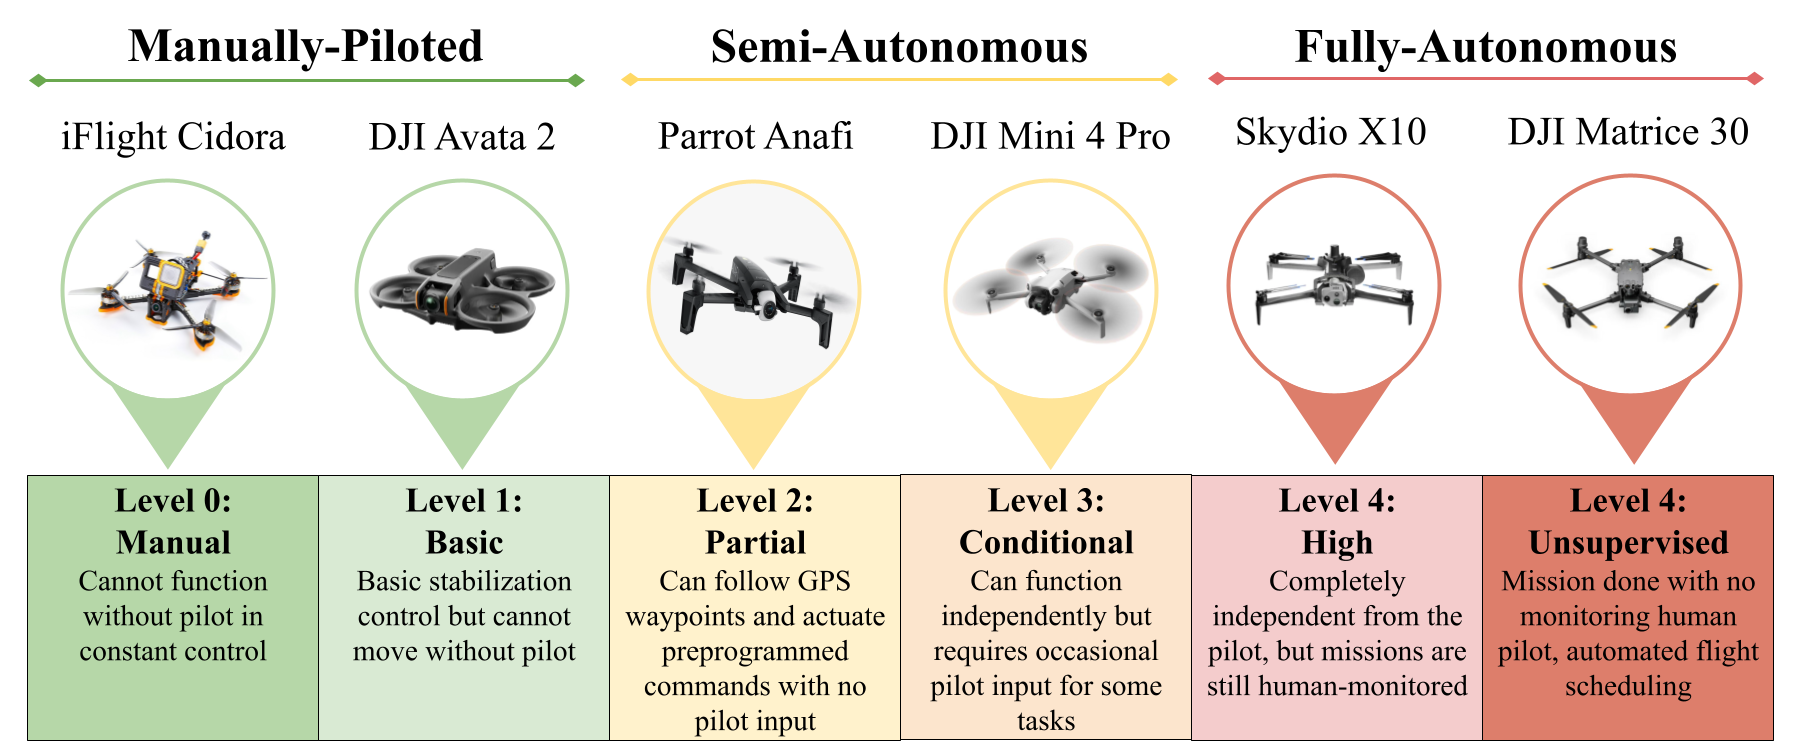
\includegraphics[width=1.0\linewidth]{chapter2/FIGS/spectrum.png}
    \begin{captext}
        \small Based on the capability set of each drone, I have roughly placed them on the theoretical spectrum of autonomy. This is an entirely subjective categorization. Others may differ on how to define each category and which drones belong in them.
    \end{captext}
    \caption{The ``Spectrum of Autonomy''}
    \label{fig:spectrum}
\end{figure}

\subsection{What is Holding Drones Back?}
\label{sec:problems}
As presented by Table~\ref{tab:drone-apps}, there are many applications where drones have been useful. However, it is my belief that they still have not lived up to their true potential. Many of the listed tasks, such as aerial surveys, building inspection, and police surveillance, are still done using full manual or human-assisted control in densely populated areas. Yet, many if not all of these tasks could benefit greatly from full-autonomy, especially in or around cities. Surveys or inspection flights could be performed daily, without human supervision, with an auto-generated report sent out for engineers to look over. This could greatly reduce costs and prevent critical infrastructure failures, potentially saving lives~\cite{Dorafshan2018}. Automated police surveillance could free up officers, reduce training overhead, and provide round-the-clock monitoring without any risk of fatigue. So why have fully-autonomous platforms failed to see widespread use in these urban applications, when they have been used with great success elsewhere?

The answer is complicated, but I believe that there are five clear problems facing fully-autonomous drones in dense urban settings: \\[0.1]
\begin{enumerate}
    \item \textbf{Weight}: fully-autonomous aircraft are heavy, as discussed in Section~\ref{sec:current-market}. This is because they require onboard compute like GPUs to operate which drive up weight. This directly clashes with most international drone regulation which becomes progressively more restrictive over 250~g. \\[0.1]
    \item \textbf{Usability}: the majority drone users have limited or non-existent programming experience. Unfortunately, most commercial fully-autonomous offerings today demand skilled programmers to operate efficiently and safely. This makes it daunting for inexperienced users to adopt a fully-autonomous platform. \\[0.1]
    \item \textbf{Versatility}: there is a major trade-off in current fully-autonomous drone products between weight and versatility. Heavy platforms which carry generalized compute hardware like CPUs and GPUs are versatile since they can run most kinds of software natively. On the other hand, lightweight platforms cannot carry generalized compute due to weight constraints, and thus usually carry specialized compute for only one or two mission types. \\[0.1]
    \item \textbf{Portability}: drone manufacturers have their own, tightly integrated software stack that does not work with other drone models. This all or nothing approach means that a consumer must stick within the hardware ecosystem or be forced to buy an entirely new fleet of drones. \\[0.1]
    \item \textbf{Cost}: fully-autonomous drones typically cost around ten times the cost of comparable semi-autonomous drones. This makes them much less economical to deploy at scale. 
    \\[0.1]
\end{enumerate}
At the time of writing this thesis, no commercial product has addressed all five of these concerns.


\section{Prior Research}
\label{sec:prior-work}
In parallel to commercial efforts, autonomous drone research has surged in recent years. Real-time execution of active vision tasks has been a key driver. Schedl et al proposed an autonomous drone design for classification-driven adaptive search and rescue in densely forested environments~\cite{Schedl2021}. George et al demonstrated a drone inspection system which could localize the drone's camera view onto a 3D model of a target structure in real time~\cite{George2019}. Chen et al showed an efficient drone onboard computation model for visual object tracking~\cite{Chen2018}. Many other projects have explored similar applications in surveillance, wildlife monitoring, racing, and obstacle avoidance~\cite{Apvrille2014,Li2020,Devos2018,Alsalam2017,Ward2016}.  

A growing number of researchers have identified some of the problems outlined in Section~\ref{sec:problems} (\textit{weight}, \textit{usability}, \textit{versatility}, \textit{portability}, and \textit{cost}) as important research areas. In this section, I will present projects that attempt to solve these problems. I will also discuss their limitations and why their solutions have not fully addressed the issues I outlined.

\subsection{Weight}
Since as early as 2009, the drone research community has recognized the importance of lightweight aircraft in real world applications~\cite{Burkle2011, Burkle2009}. Lightweight ($\leq 450$~g) autonomous drones have many benefits over their heavier counterparts: they are safer to operate, have simpler transportation logistics, and have a lower noise profile. It was theorized that achieving such lightweight autonomy would enable the vision of cooperative drone swarms~\cite{Floreano2015}. Since the mid 2010s, much work has focused on bringing high-level autonomy to small, lightweight drones. Schmid et al proposed a sub-1~kg aircraft design which could perform unassisted visual navigation~\cite{Schmid2014}. Palossi et al developed visual navigation and human pose estimation software which runs onboard 27~g drones~\cite{Palossi2019,Palossi2021}. M{\"u}ller et al demonstrated a depth-based obstacle avoidance system for 35~g drones~\cite{Muller2023}. Many of these projects suffer from similar issues of \textit{portability}. That is, they either use purpose-built aircraft or function on one type of aircraft. There is little ability to deploy these systems to different drone hardware, a serious drawback in an ever-changing drone landscape. 

\subsection{Usability}
\label{sec:development-platforms}
For many years, drone research did not consider usability. Many projects used custom-built aircraft with no guidance on how to replicate the platform for other researchers. Others provided autonomous software which was only usable by experts, and thus could not be leveraged by average developers. These days, the drone research community has started to recognize the importance of usability. Beseda et al presented a mission-oriented control infrastructure for easily managing swarms of autonomous UAVs~\cite{Besada2019}. Mottola et al proposed a simple but expressive API for drone team control~\cite{Mottola2014}. Tilley et al developed a block programming language that could allow children to program autonomous drones~\cite{Tilley2017}. While this work is useful, these projects do not present a practical integration strategy with real consumer drones. There is no consideration of \textit{portability} or \textit{weight}, both very important for public deployment.

\subsection{Versatility}
Mission versatility is a feature that most heavy fully-autonomous drones already possess, since they carry generalized compute like CPUs and GPUs which can run GPLs (general-purpose programming languages) and inference deep neural networks with relatively low latency. However, achieving this versatility on lightweight drones is an enduring challenge. This is because miniaturizing generalized compute hardware is difficult, and weight-optimized compute hardware is inflexible~\cite{Hu2022}. Still, many have tried to modify lightweight onboard hardware to be able to run heavyweight computer vision. Albanese et al propose a neural accelerator modification to a Raspberry Pi which could be flown onboard small UAVs~\cite{Albanese2022}. Zhang et al demonstrate an FPGA architecture for drones that can inference neural networks with much lower power demand than GPUs~\cite{Zhang2022}.

\begin{figure}
    \centering
    \subfloat[\centering Bitcraze Crazyflie\\(27~g)]
    {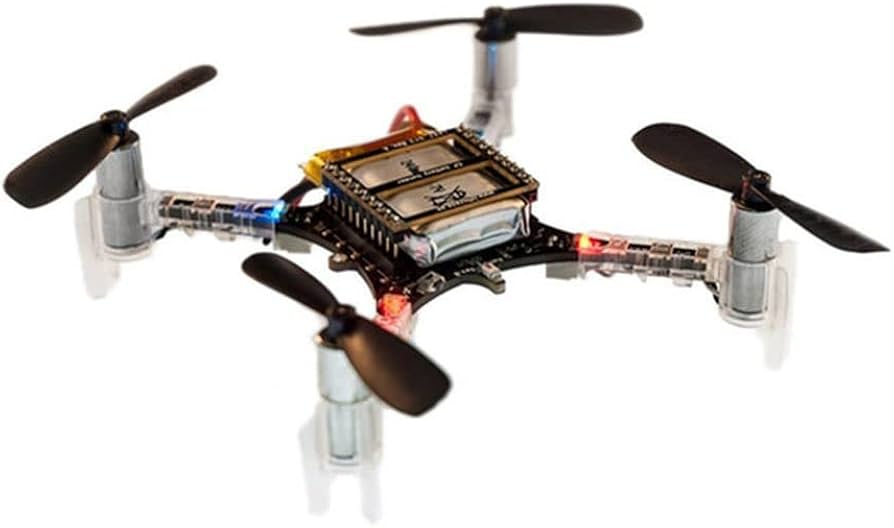
\includegraphics[width=0.30\textwidth, height=1.5in]{chapter2/FIGS/crazyflie.jpg}}
    \qquad
    \subfloat[\centering Modal AI Starling\\(280~g)]
    {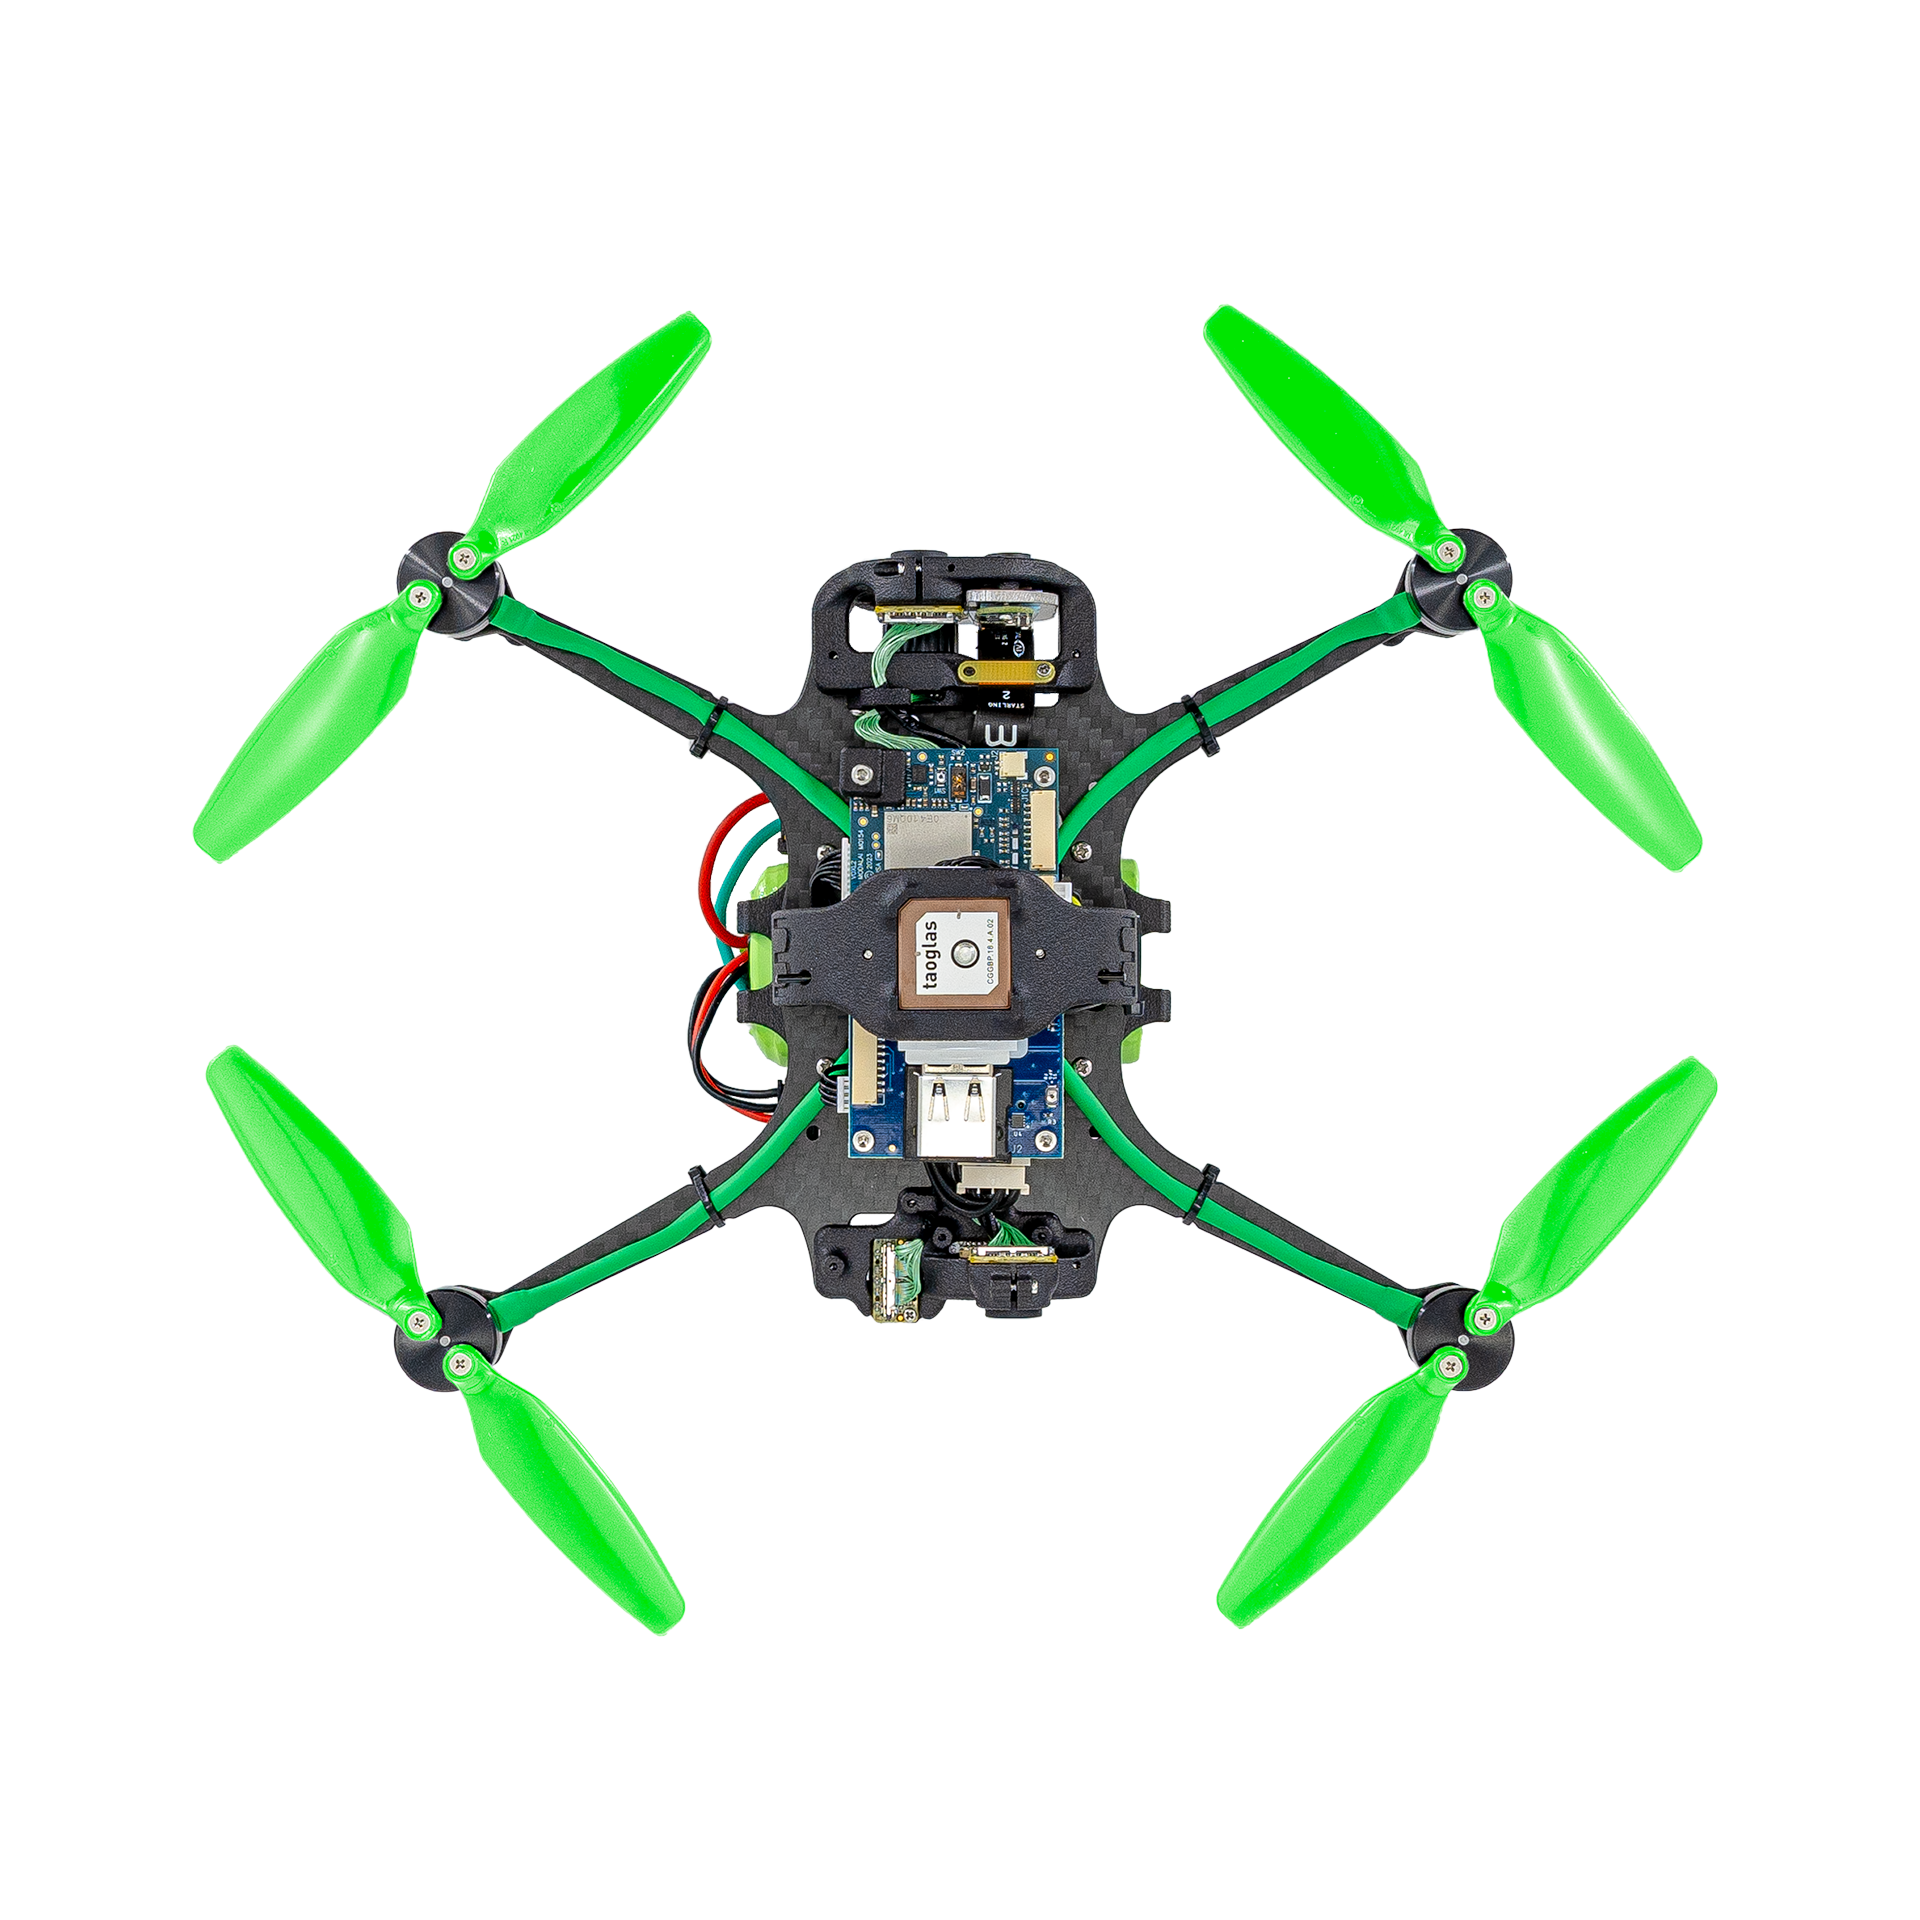
\includegraphics[width=0.30\textwidth, height=1.75in]{chapter2/FIGS/starling-2.png}}
    \caption{Consumer Drone Development Platforms}
    \label{fig:drone-dev-platforms}
\end{figure}

\subsection{Portability}

\subsection{Cost}

\section{A Key Insight: the Onboard Compute Trade-off}
\label{sec:better-autonomous-drones}
The key factors of \textit{weight}, \textit{usability}, \textit{versatility}, \textit{portability}, and \textit{cost} all hinder autonomous drone development and deployment, yet no proposed system has solved all of these issues simultaneously. Central to this problem is the trade-off between heavy, generalized, onboard compute that supports common programming ecosystems but exceeds regulatory limits, and lightweight, specialized, onboard compute that can only run tailor-made programs, but is light enough to fly within regulatory bounds. 





\chapter{Connecting COTS Drones to the Edge}
The key factors of \textit{weight}, \textit{accessibility}, \textit{versatility}, \textit{portability}, and \textit{cost} all hinder autonomous drone development and deployment, yet no proposed system has solved all of these issues simultaneously. Clearly, significant research effort has been spent on solving these problems; so why does no such system exist? Central to the answer is what I call the \textit{onboard compute trade-off}. The onboard compute trade-off is a property of unmanned aerial platforms that claims:

\begin{displayquote}
Traditional hardware, like CPUs and GPUs, offers the benefit of versatile, software portable, cost-effective compute power at the expense of weight. Specialized hardware offers the benefit of light weight at the expense of versatile, software portable, cost-effective compute power. Thus, in order to reduce weight, \textit{versatility, portability, and cost must be compromised}.
\end{displayquote}

This fact has limited the development of lightweight fully-autonomous drones and it is chiefly responsible for the gap that exists in the drone market today. Unfortunately, even with recent technological advances, it is unclear whether this challenge can be solved. But, there may be ways it can be circumvented. 

In this chapter, I will introduce SteelEagle, a drone autonomy system designed to bring intelligence to lightweight, commercial-off-the-shelf (COTS) drones. SteelEagle skirts the need for heavy onboard compute by leveraging edge computing, a computational model that involves offloading work from a less powerful device over a low latency network link to a nearby powerful device which finishes the work and returns the result. In this way, SteelEagle aims to solve the onboard compute trade-off and lower the weight-barrier to drone autonomy. In Section~\ref{sec:advent-edge}-\ref{sec:init-hardware}, I explain the background and prior research that drove the creation of SteelEagle. In Sections~\ref{sec:achieving-cell-conn}-\ref{sec:quest-working-stream}, I discuss the many failed prototypes I tested before arriving at an initial working solution.

\section{The Advent of Edge Computing}
\label{sec:advent-edge}
Over the past few years, a new computational paradigm has emerged called \textit{edge computing}. Edge computing gives mobile devices access to strong computational resources at low latency by offloading to a network-proximal server~\cite{Satya2017}. In many ways, this is similar to cloud computing. The theory is that mobile devices will always be resource-poor compared to data centers. By sending compute jobs over the network, running on the vast compute of a data center, and getting the result back, mobile devices can mitigate their computational deficiencies. 

The insight of edge computing is that some computation is \textit{latency-sensitive}. That is, the faster the result is returned to the user, the better the system performs. This is usually the case for interactive applications, like augmented reality, or for reactive applications, like robotic actuation in response to visual stimuli. In these cases, sending a compute job to the cloud may be too slow. Edge computing positions smaller groups of servers, called cloudlets, physically closer to mobile clients, usually co-located with cell towers. This hugely decreases latency without sacrificing much per-user compute power, since cloudlets, due to their smaller reach, have fewer tenants than cloud servers~\cite{Charyyev2020,Dolui2017}.

\begin{figure}
    \centering
    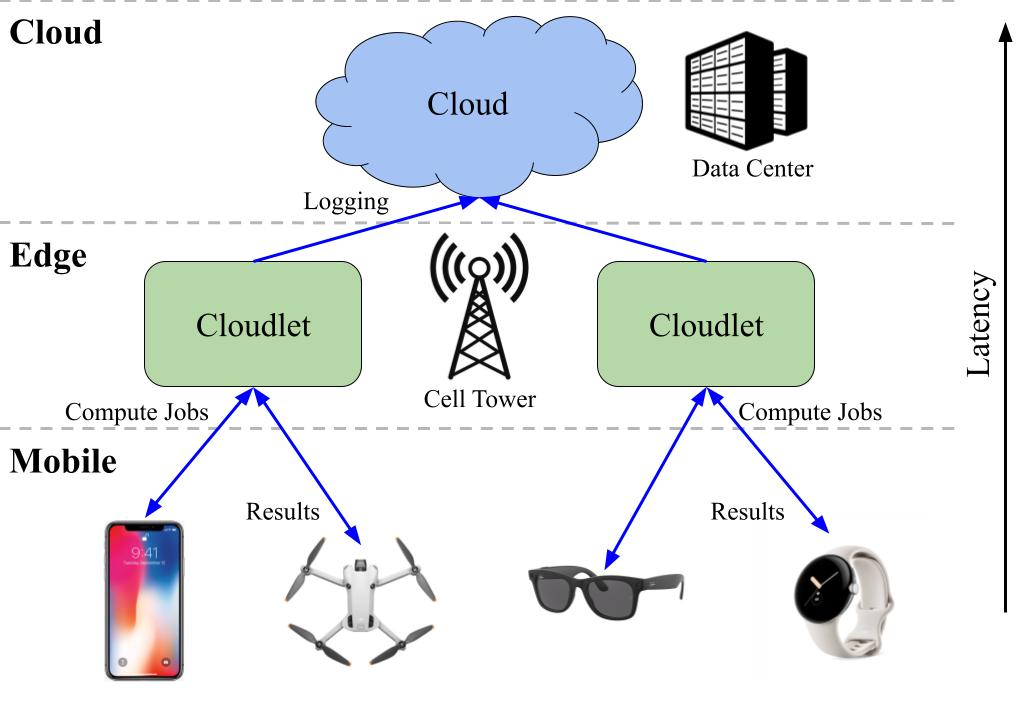
\includegraphics[width=0.9\linewidth]{chapter3/FIGS/edge-computing.jpg}
    \caption{Edge Computing Paradigm}
    \label{fig:edge-computing}
\end{figure}

\section{Autonomous Drones and the Edge}
\label{sec:drone-and-the-edge}
Edge computing offers a compelling alternative to the onboard compute trade-off. Instead of miniaturizing compute to fly with a drone, it is much easier to relocate heavyweight compute to the edge so that it is accessible with low latency. This has a number of important advantages over traditional onboard computation paradigms:

\begin{itemize}
    \item The underlying hardware where compute runs is well-understood and general purpose (server-grade CPUs and GPUs). This hugely increases portability and offers a developer-friendly programming environment.
    \item The cost of edge-enabled drones is low; there is no longer a need for expensive lightweight compute hardware, only a relatively cheap modem to communicate with the edge. This greatly increases scalability and thus the economic viability of drone swarms.
    \item Server-grade compute power will always vastly exceed mobile compute power~\cite{Qi2012}. This opens the door to real-time inference of heavy models like transformers~\cite{Vaswani2017}.
\end{itemize}

An edge computing approach is not without its drawbacks. The drone is now fully reliant on its communication link with the cloudlet, meaning it is susceptible to service disruptions and bandwidth constraints. This is no worse than manually-piloted drones, which are also dependent on a communication link to the RPIC. Still, these factors must be accounted for in any successful edge-based drone system.

Edge-enabled drones are not a new idea. For several years, researchers at the intersection of edge computing and robotics have published many influential papers on the topic~\cite{Wang2017,Bertizzolo2020,Asaamoning2021,Gharibi2016}. In
these projects, drones use a ground station or cloudlet in conjunction with other nearby aircraft to offload high compute loads. However, this previous work either focused on the theory of how such a system should be designed or on solutions using custom components. None identified weight as a major constraint, and so they failed to present a practical, fully-functional system for public flight operations.

\begin{figure}
    \centering
    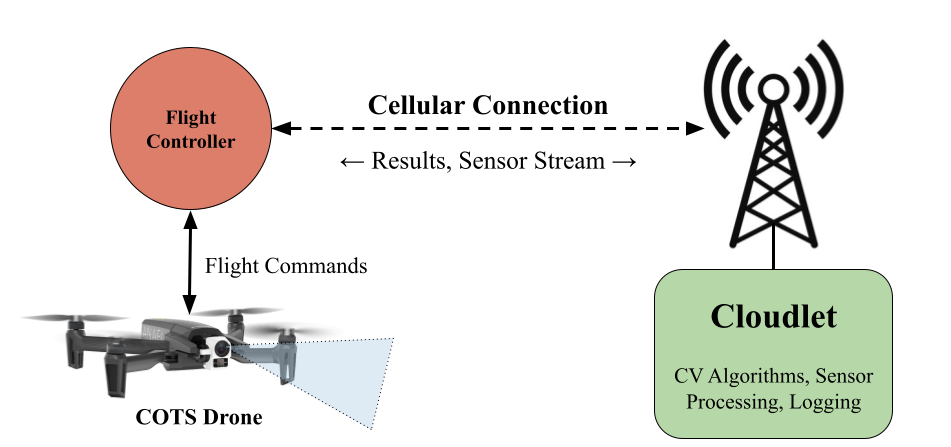
\includegraphics[width=1.0\linewidth]{chapter3/FIGS/simplearch.png}
    \caption{SteelEagle Autonomy Model}
    \label{fig:steeleagle-model}
\end{figure}

\section{SteelEagle: Inducing Autonomy on Lightweight Drones}
\label{sec:se-intro}
I introduce \textit{SteelEagle}, a drone-agnostic framework for inducing full autonomy on lightweight drones using edge computing. In contrast to previous work, SteelEagle is built on top of commercial-off-the-shelf (COTS), semi-autonomous, photography drones (\S\ref{sec:current-market}), which are supplemented with a 4G~\cite{ETSI} connection to the edge to provide the computation needed for fully-autonomous operation (Figure~\ref{fig:steeleagle-model}). COTS photography drones are typically cheaper, more accessible, and much lighter than fully-autonomous platforms. With this approach, SteelEagle presents the best of both worlds: lightweight, cheap drones with powerful real time computation capabilities. SteelEagle's backend also supports a plug-and-play approach, allowing developers to swap out underlying drone hardware form beneath its abstraction layer. This makes the system highly portable and versatile, able to adapt to the rapid pace of AI innovation. With respect to the challenges outlined earlier (\S\ref{sec:problems}), SteelEagle addresses them all:

\begin{itemize}
    \item \textbf{Weight}: SteelEagle is designed to work with lightweight, commercial-off-the-shelf (COTS) photography drones, many of which are under 400~g. These drones typically would be categorized as semi-autonomous, but edge offloading enables them to become fully autonomous.
    \item \textbf{Accessibility}: COTS photography drones are designed to be accessible, since they are marketed to everyday consumers. Thus, they are much easier to work with and safer to fly. In addition, the programming environment and abstractions provided by SteelEagle make it easy to develop new drone applications.
    \item \textbf{Versatility}: SteelEagle's edge backend runs on traditional compute hardware which ensures maximum versatility and full access to popular AI libraries like PyTorch. This encourages rapid development and evolution through preexisting AI tool chains. It also eliminates the  need to squeeze models onto constrained drone hardware.
    \item \textbf{Portability}: SteelEagle abstracts away drone-facing hardware and has no restrictions on the drone control stack. This promotes portability and makes SteelEagle drone-agnostic.
    \item \textbf{Cost}: COTS photography drones are some of the most cost-optimized drones on the market, due to their target mass-market audience. As a result, the unit cost for SteelEagle drones can be several orders of magnitude lower than typical fully-autonomous platforms.
\end{itemize}

As with all edge-based systems, SteelEagle must plan for and adapt to changing network environments. More critically, its performance on common drone tasks like object tracking and obstacle performance must come close to matching that of existing autonomous drones to be useful, despite bandwidth and latency challenges inherent in offloading solutions.

\section{Design Goals of SteelEagle}
Establishing a connection to the edge on any current COTS drone hardware is non-trivial. Doing so on a COTS photography drone is near impossible out-of-the-box. This is the case for the following reasons:
\begin{itemize}
    \item Photography drones are tightly-integrated, black boxes with no ability to change onboard software or hardware. This is because they are meant to be used by novice pilots and so they simplify the user experience at the cost of customizability.
    \item Photography drones usually require a constant connection to the pilot via a controller. This not only mandates a human-in-the-loop but also prevents BVLOS operation.
    \item Photography drones are not designed to carry much payload. They provide no means to power any payload either since their batteries are closed off during flight.
\end{itemize}
These are challenges that any prototype must overcome, regardless of underlying drone platform.

For SteelEagle, drones connect to the edge over public 4G/5G cellular. Cellular has excellent coverage in populated areas, support for device mobility, and favorable penetration characteristics~\cite{FCC}. This ensures good service wherever SteelEagle drones fly, especially in urban or suburban settings. Unfortunately, at the time of writing this dissertation, no lightweight COTS photography drones are equipped with cellular connectivity; they are designed to be operated within visual line-of-sight of a pilot, a task for which WiFi or RC is well-suited. For my prototype to work, I will have to bring cellular connectivity to a COTS drone without modifying its internal components.

\section{Initial Hardware}
\label{sec:init-hardware}
For my initial prototype, I chose to work with the Parrot Anafi~\cite{ParrotAnafi}. The Anafi is a COTS photography drone that weighs 320~g and costs \$470. It is equipped with an autopilot that can follow GPS waypoints and perform automatic stabilization. This stabilization involves increasing thrust of rotors to compensate for wind, allowing the drone to maintain its position even in windy conditions. Table~\ref{tab:anafi-features} shows a more detailed specification of the aircraft.

\begin{figure}
    \centering
    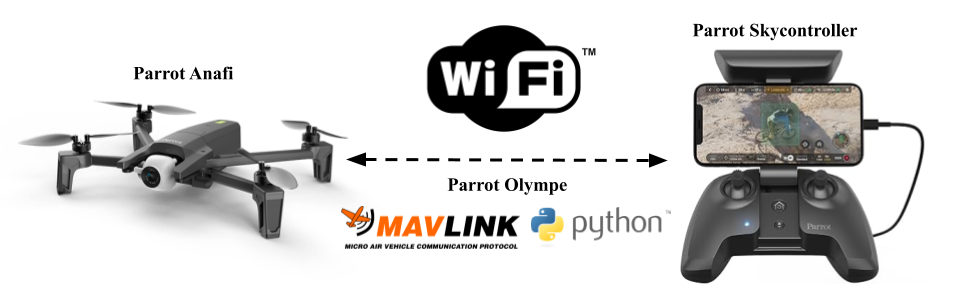
\includegraphics[width=1.0\linewidth]{chapter3/FIGS/ctrl.png}
    \caption{Parrot Remote Control Setup~\cite{ParrotAnafi}}
    \label{fig:parrot-control-setup}
\end{figure}

\begin{table}[]
    \centering
    \rowcolors{2}{gray!10}{white}
    \begin{tabular}{|c|c|}
     \hline
     \textbf{Feature} & \textbf{Description}  \\
     \hline
     Weight & 320~g \\
     \hline
     Cost & \$470 \\
     \hline
     Flight Time & Up to 25 min, in reality 20 min \\
     \hline
     Camera & 4K photo/video \\
     \hline
     Video Stream & 720p 30fps \\
     \hline
     Autopilot* & Custom \\
     \hline
     API & Parrot Olympe / GroundSDK \\
     \hline
     Connectivity & WiFi \\
     \hline
    \end{tabular}
    \caption{Parrot Anafi Specifications}
    \label{tab:anafi-features}
\end{table}

\subsection{Control Scheme}
The Anafi is designed to be controlled by a human pilot using a remote controller with an attached mobile phone (the Parrot Skycontroller) or exclusively using a mobile phone over WiFi. Alternatively, the drone can also be controlled over WiFi with a Python API called Parrot Olympe or an Android API called Parrot GroundSDK. They are based on the ubiquitous MAVLink protocol~\cite{MAVLink}. Both these APIs grant users high-level flight control and access to telemetry.

Olympe and GroundSDK support two main command types: manual and guided. Manual commands directly actuate the drone. For instance, moving the left stick upwards on the controller would send a manual command to ``increase throttle''. Guided commands, on the other hand, provide the drone with a target to actuate towards. For example, a ``move to GPS location'' message is a guided command since the drone self-actuates towards the specified target.

\subsection{Networking}
The drone hosts a WiFi network which supports up to two attached clients. A controller must connect to the WiFi network in order to talk to the drone. This channel may be configured to be either 2.4~GHz or 5~GHz. As reported by Parrot, the connection range of the WiFi channel is around 4~km~\cite{ParrotAnafi}. From my testing, this can fall to around 0.5~km in areas with high wireless interference.

\subsection{Video Stream}
A 720p 30fps video stream is generated by the drone and transmitted on its WiFi network via the real-time streaming protocol (RTSP)~\cite{RTSP}. The settings of this stream are not configurable. It is encoded using an intra-refresh slice-decode scheme which is designed to be resilient to packet loss~\cite{Cloudinary}. I will cover the drone's video stream in more detail in Section~\ref{sec:anatomy-drone-stream}.

\subsection{Magnetometer}
Most drones are equipped with a magnetometer for discerning bearing. The Parrot Anafi has an unusually sensitive magnetometer. If the drone's magnetometer detects sufficient interference (e.g. caused by nearby ferromagnetic material~\cite{Ardupilot}), it refuses to fly any guided commands and cancels any guided actuation. This is for safety; if the drone does not have an accurate understanding of its bearing, it may not actuate correctly towards its target and therefore increase the probability of a crash.

\section{Achieving Cellular Connectivity}
\label{sec:achieving-cell-conn}
The Parrot Anafi, like most photography drones, only supports WiFi connectivity and mandates a constant connection to the pilot controller. As stated earlier, the goal of SteelEagle is to use this drone without modification and with an entirely COTS payload.  Thus, any prototype must operate within these constraints. In order to integrate a cellular connection into the loop, it must ensure that from the drone's perspective, it is always connected to what it thinks is a human pilot. One possibility is to mount a router-like device onboard which connects to the drone WiFi and also maintains a cellular connection to the edge. Such a device would have to be light enough to fly but also would need to be able to power itself for the duration of a flight. Ideally, it would also have some internal compute so it can still control the drone during brief network outages.

\subsection{Mobile Phone}
In the COTS mobile device space, one of the best SWaP (size, weight, and power) optimized devices is the mobile phone. Mobile phones have grown immensely powerful in recent years, with some rivaling the power of laptop computers. Furthermore, they are lightweight (usually under 200~g), have a full-featured software development environment, and can power themselves for several hours, even under load. Their connectivity over WiFi and cellular is highly reliable and extensively tested.

In the context of the Parrot Anafi, an Android phone would work well for this purpose, since the Anafi supports an Android API, Parrot GroundSDK. This motivates the following model: an Android phone flies onboard the Parrot Anafi, acting as both a router and a stand-in for the remote controller. By running GroundSDK, the phone will work within the Parrot ecosystem and will therefore maintain the pilot connection that the drone necessitates (Figure~\ref{fig:phone-control}). To save weight, I selected one of the lightest widely-available Android phones on the market for this task: the Google Pixel 4a. The Pixel 4a weights 143~g and has both 4G and 5G connectivity.

\begin{figure}
    \centering
    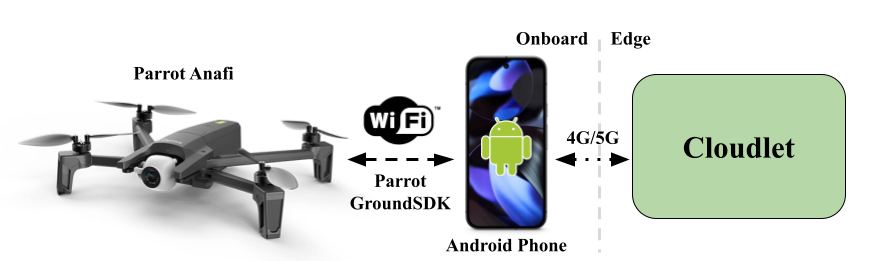
\includegraphics[width=1.0\linewidth]{chapter3/FIGS/onboard-phone.png}
    \caption{Android Phone Control~\cite{ParrotAnafi}}
    \label{fig:phone-control}
\end{figure}

Now that I had selected a device, it was time to mount it onboard the drone. For my initial mount, to save weight, I used industrial strength velcro and rubber bands. The drone was able to fly autonomously with the phone onboard and offload its video stream to the edge. However, I observed strange flight characteristics which caused several crashes. Upon further investigation, I determined that the phone was interfering with the magnetometer on the drone. This was causing the drone to lose track of its bearing mid-flight and veer off course.

To solve this magnetic interference, I added a layer of EMI  (electro-magnetic interference) shielding between the phone and the drone chassis. The shielding was made of Mu-metal, a nickel-iron ferromagnetic alloy used to absorb electro-magnetic radiation~\cite{Orasugh2023}. After testing, I determined that this mostly negated the observed interference. Unfortunately, it also added significantly to the payload weight, so much so that it exceeded the maximum takeoff mass (MTOM) of the aircraft. Once an aircraft's payload surpasses MTOM, it cannot fly because the lift it generates is no longer greater than its weight. Even with the lightest Android smartphones available, like the 61~g Unihertz Jelly Pro, the added weight of EMI shielding exceeded the Anafi's MTOM. 

As a result of the interference and MTOM restrictions, I was forced to abandon the phone prototype. It was too heavy for the Parrot Anafi hardware. I began searching for an alternative COTS device, much lighter than the Pixel 4a, but with the same broad specifications (self-contained, WiFi and cellular, self-powered, able to run Parrot GroundSDK or Olympe). 

\subsection{Smartwatch}
While mobile phones are the best SWaP-optimized devices on the market, smartwatches are by far the lightest, self-contained, commercially available computers. For many years, they were designed to operate in tandem with a phone, acting as a kind of always-visible secondary display. As time progressed, smartwatches grew more independent, incorporating more connectivity options and mounting more internal compute. The fitness community was a driving force behind this transformation. Many runners, for example, wanted a very small, lightweight, wearable device that could track their progress, contact emergency services, and play music on the move. In the late 2010s and early 2020s, this resulted in smartwatch products with cellular connectivity and enough local compute to run basic applications.

In many ways, smartwatches are the perfect device for SteelEagle's use case. They are extremely lightweight (less than 30~g compared to over 100~g for a phone), self-powered, cellular and WiFi-enabled, and able to run a slimmed-down Android (WearOS). For my smartwatch-based prototype, I chose the Samsung Galaxy Watch 4. At the time, this was the lightest cellular-capable Android smartwatch available. The Samsung Galaxy Watch 4 weighs just 25~g.

\begin{figure}
    \centering
    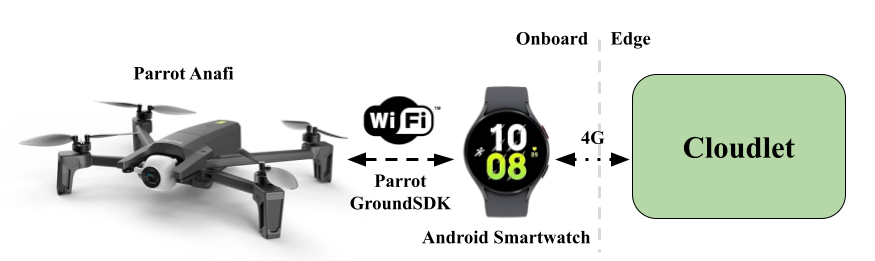
\includegraphics[width=1.0\linewidth]{chapter3/FIGS/onboard-watch.png}
    \caption{Android Watch Control~\cite{ParrotAnafi}}
    \label{fig:watch-control}
\end{figure}

After porting Parrot GroundSDK to WearOS, I was able to establish a 4G connection from the edge to the watch while autonomously piloting the drone via onboard software (Figure~\ref{fig:watch-control}). Now, all that was left to do was to physically mount the watch on the drone. I used a 3D-printed harness for this task, which clips onto the Parrot Anafi's removable battery. The harness weighs an additional 14~g, bringing the total payload weight to 39~g. Figure~\ref{fig:harness} shows the full assembly mounted on the aircraft. This brings the total take-off weight to 359~g, just 109~g above the 250~g FAA regulation threshold. Through rigorous testing, I determined that the watch payload did not exhibit the same negative flight characteristics as the Pixel 4a payload. It did not create as much EMI, likely because of its smaller size and lower power draw, and thus no shielding was needed. Additionally, the weight of the payload was far below the Anafi's MTOM, even with the added 3D printed mount to securely fasten it onboard.

The Samsung Galaxy Watch 4 finally yielded a successful prototype. The watch payload was able to autonomously fly the drone while maintaining a cellular connection to the edge. However, much work still remained unfinished. In particular, the drone's RTSP video stream would need to be transmitted to the edge in order to run the AI algorithms responsible for true autonomy: object detection, image segmentation, and obstacle avoidance among others. This would prove to be a formidable obstacle that pushed the watch hardware to its limit.

\begin{figure}
    \centering
    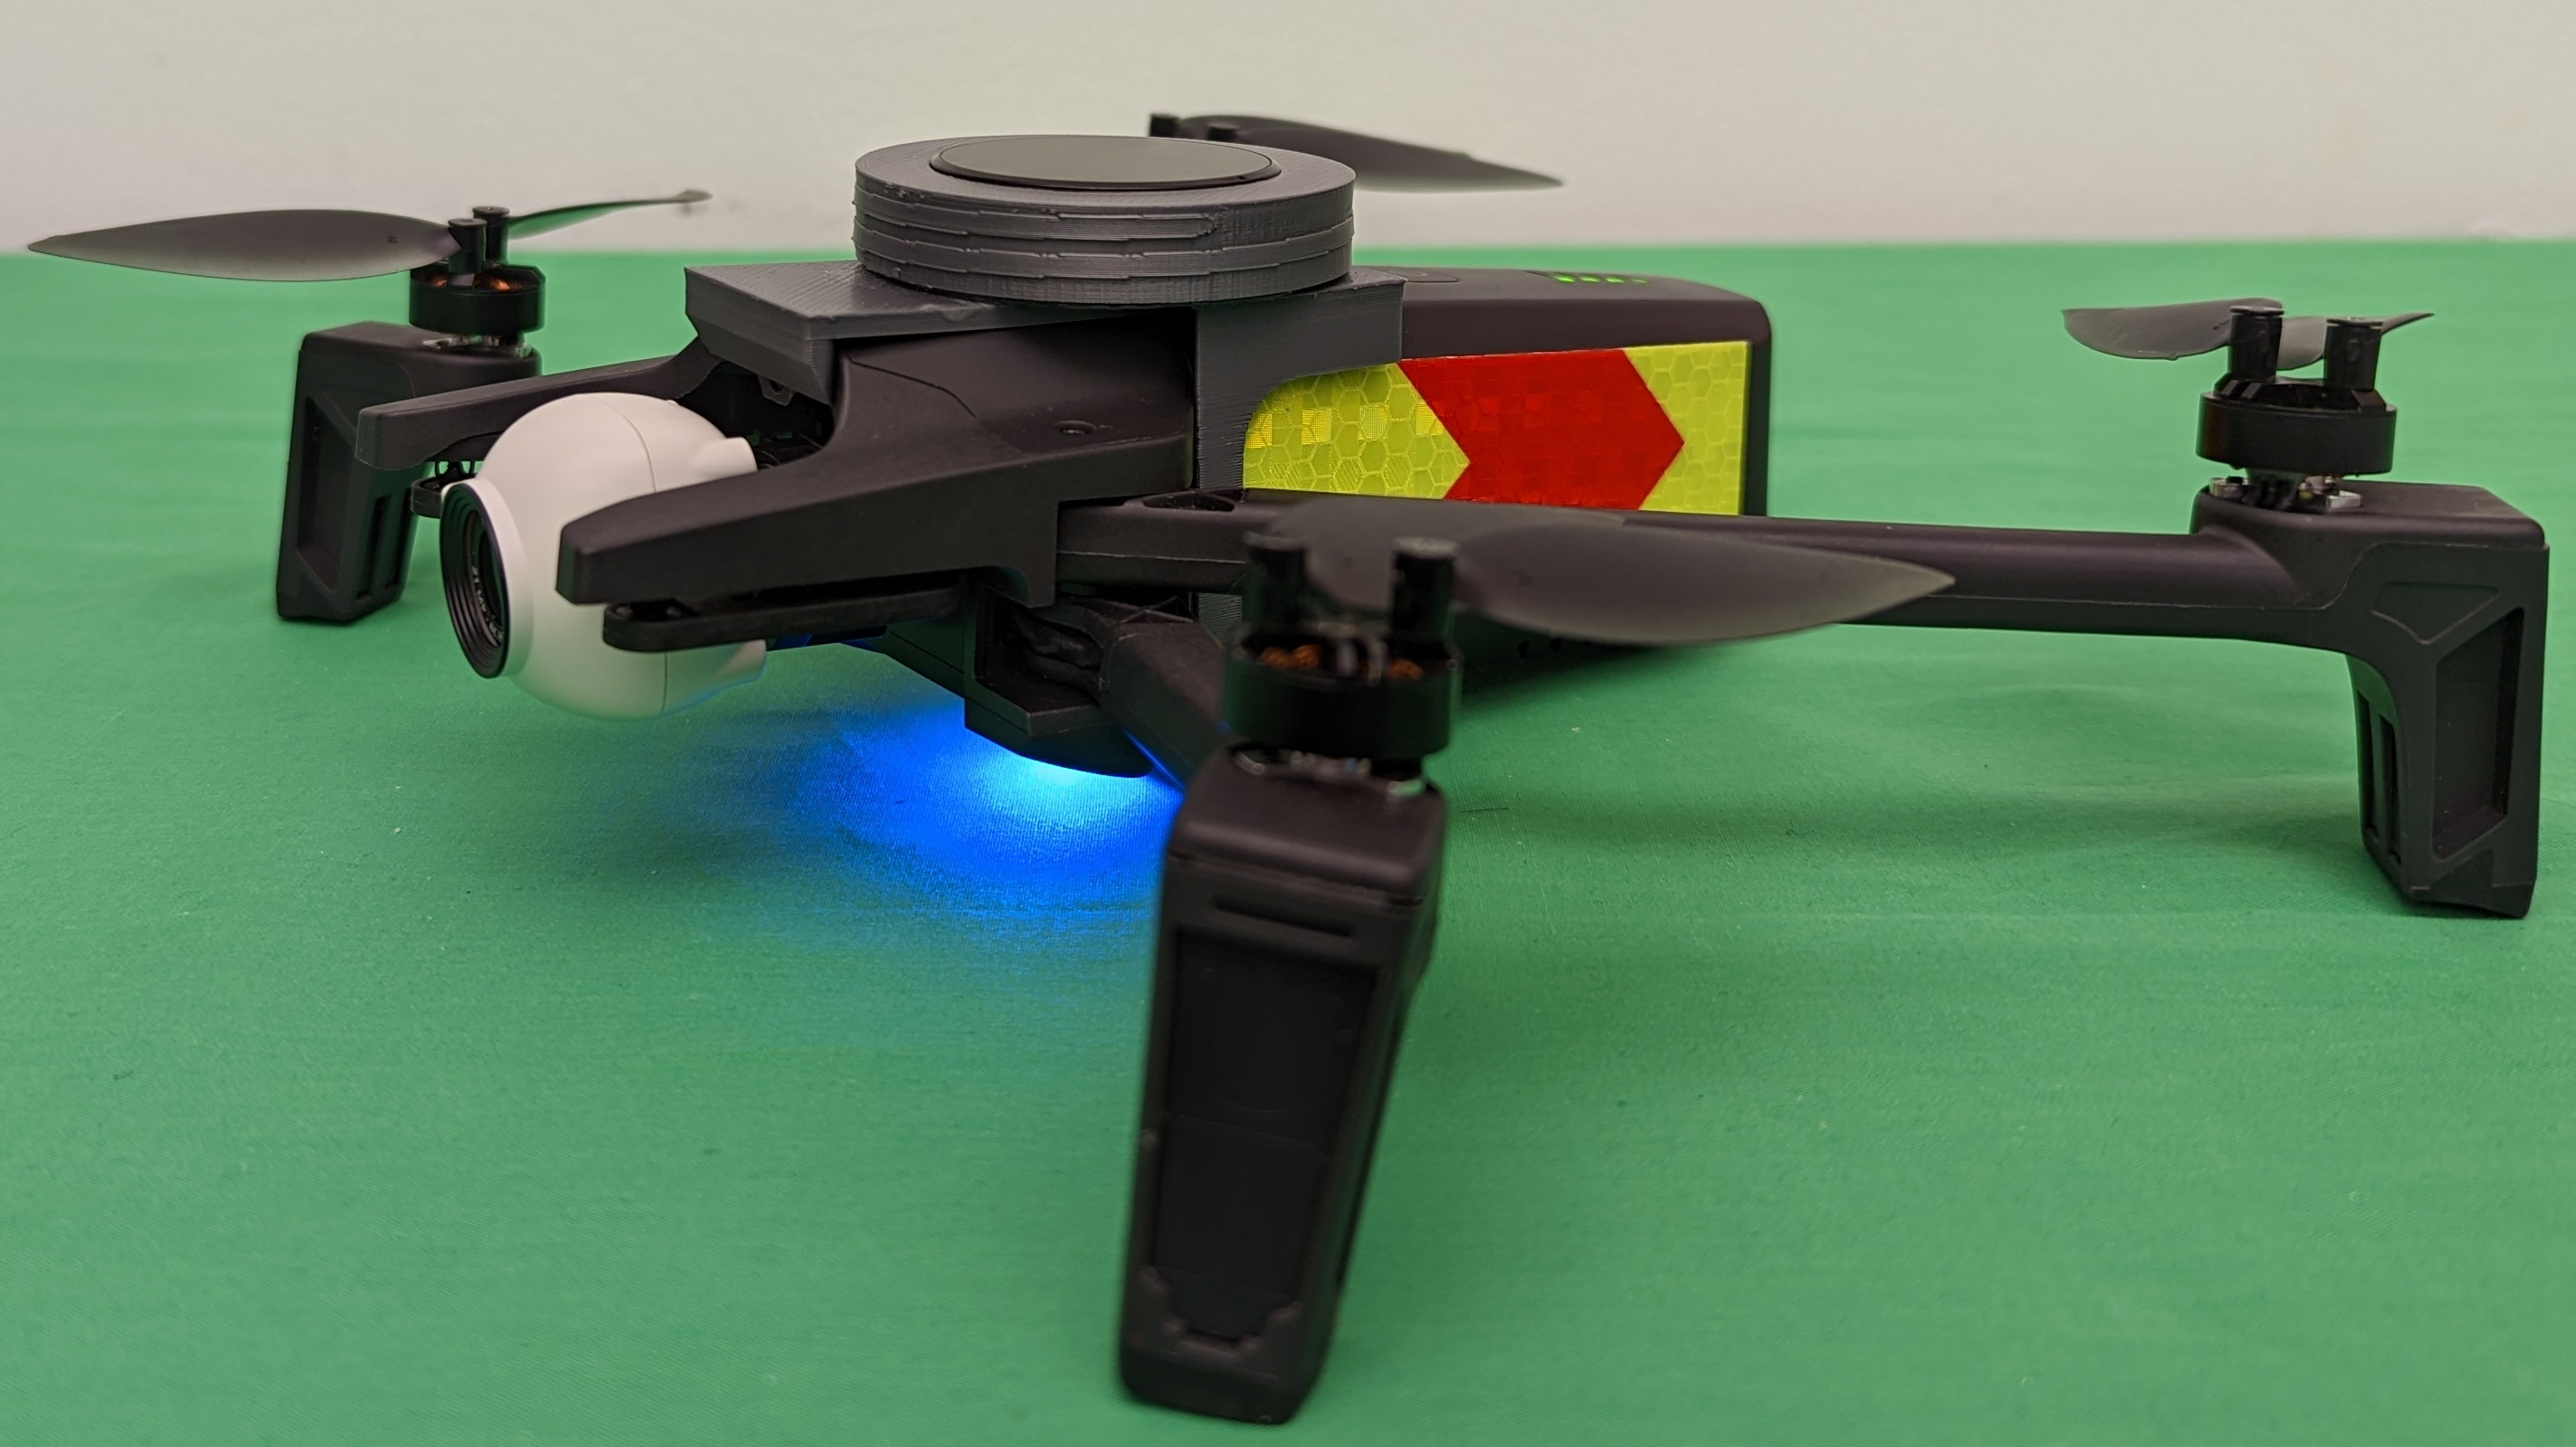
\includegraphics[width=0.6\linewidth]{chapter3/FIGS/drone-watch-combo.jpg}
    \caption{Drone with Watch-Harness Payload}
    \label{fig:harness}
\end{figure}

\section{An Austere Computing Environment}
\label{sec:austere-computing}
The watch is an austere computing environment with a dual-core
1.18~GHz ARM Cortex-A55 processor, 1.5 GB RAM, and 16 GB flash.
Table~\ref{tab:austerity} compares its attributes to the Google Pixel 4a and to the Unihertz Jelly Pro, the lightest-available Android smartphone. As wearable hardware, the watch has stringent thermal protection to shut itself down if its temperature approaches hardware limits. In addition, since wearables are meant to be worn, these hardware temperature limits must be much lower than traditional computers to prevent skin burns~\cite{Hepokoski2021}. Both computing and network transmission cause watch temperature to rise significantly.

This is a major problem, especially since in my design, the watch offloads the drone video stream to the edge. Typically, streaming tasks are both compute and transmission intensive. The act of sending frames too often or decoding frames onboard could cause overheating. In the case of the Samsung Galaxy Watch 4, overheating is detected by the operating system which in turn triggers a thermal shutdown. If this occurs, all currently running applications are suspended and the watch goes into hibernation until it is cool enough to proceed. A thermal shutdown in-flight would turn off the Parrot GroundSDK software running onboard and would thus trigger a pilot disconnection event on the drone. When this occurs, the drone returns automatically to its takeoff GPS location and lands. While this is far from disastrous, it would certainly be a serious handicap. As a result, the watch must be conservative in its network transmission and onboard computation in order to prevent overheating.

On the other hand, the agility and accuracy of the computer vision algorithms running at the edge are critically dependent on the attributes of the video stream. These algorithms determine the overall performance of the system; they are the ``brain'' that enables fully-autonomous operation. If the video stream delivered to them is hindered, performance will be directly affected. In order for this system to be effective, the watch must deliver as high fidelity a stream to the edge as possible without compromising its thermal limits. This is a delicate balancing act.

\begin{figure}
\centering
\begin{tabular}{|l|c|c|c|}
\hline
    & Samsung & Unihertz & Google \\
    & Galaxy & Jelly & Pixel\\
    & Watch 4 & Pro & 4a \\
\hline
Weight & 26~g & 61~g & 143~g\\
CPU cores & 2 & 4 & 8 \\
CPU speed & 1.18~GHz&1.45~GHz & 2.2~GHz\\
Memory & 1.5~GB & 3~GB & 6~GB\\
\hline
\end{tabular}
\caption{Austerity of Mobile Hardware}
\label{tab:austerity}
\end{figure}

\section{Anatomy of the Parrot Anafi Video Stream}
\label{sec:anatomy-drone-stream}
The Parrot Anafi produces an encoded 720p 30fps video stream. It is produced on the drone's hardware and thus \textit{cannot be modified}. It is generated over the drone's WiFi network and can only be consumed by a single client on the network. Unlike most video streams, this stream uses an \textit{intra-refresh slice-decode} encoding scheme. An intra-refresh slice-decode encoding scheme is a streaming paradigm designed to minimize the visual impact of packet loss. 

To understand this special encoding scheme, first consider a normal H.264 video stream. The encoding scheme for these streams involves two types of data: complete frames (I frames) and inter frames (P and B frames). A complete frame is a full photo capture of a moment in time. When a complete frame is transmitted, it typically requires no additional data to decode. The trade-off is that complete frames are bandwidth hungry. An individual 720p complete frame can be several KBs of data. By contrast, inter frames only capture the \textit{change from the previous frame}. They require reference data in order to decode, and are meaningless on their own. Their advantage is that they are very bandwidth efficient, sometimes on the order of a few hundred bytes in size. An H.264 video stream operates by transmitting a complete frame followed by a set amount of inter frames before looping back. This preserves fidelity by smoothing out gaps between complete frames with inter frames but also preserves bandwidth by sparingly transmitting complete frames.

There is one major negative of typical H.264 video streams in the context of mobile devices: they are not resilient to packet loss. On the Internet, which is a mostly wired network, this is not a serious problem. But, over the air, packet loss is frequent. If a complete frame is lost, viewing or processing of this kind of stream must be skipped until a new complete frame can be broadcast; all following inter frames will have no complete frame to refer to and will be rendered useless. Usually this can take a whole second or more, during which a drone pilot, for example, would not be able to see.

An intra-refresh slice-decode scheme takes a different approach. Instead of complete frames and inter frames, this scheme splits a single frame into \textit{slices}. These slices capture a sliver of data horizontally across a frame. When a frame is transmitted, the encoder allocates one slice to be the ``complete slice'' (I slice) and the rest to be ``inter slices'' (P slices). Figure~\ref{fig:slice-encoding} shows a breakdown of how each set of frames transmitted by the Anafi are organized. Each inter slice is only dependent upon its section of the frame; they are completely independent of each other. 

This has two positive attributes. The first is that this minimizes the impact of packet loss on a single frame. If a single frame is dropped, only one slice of the frame loses its complete slice reference. In this case, that section of the frame is corrupted until a new complete slice is sent. Otherwise, the rest of the frame is decoded normally. The second benefit of this approach is that it keeps bandwidth usage consistent. With a traditional stream, bandwidth usage spikes when complete frames are sent but then plummets when inter frames are sent. In this scheme, since every frame has approximately the same size (one complete slice with the rest being inter slices), bandwidth usage stays somewhat constant. This is useful because other applications can now plan around its tight usage bound.

\begin{figure}
    \centering
    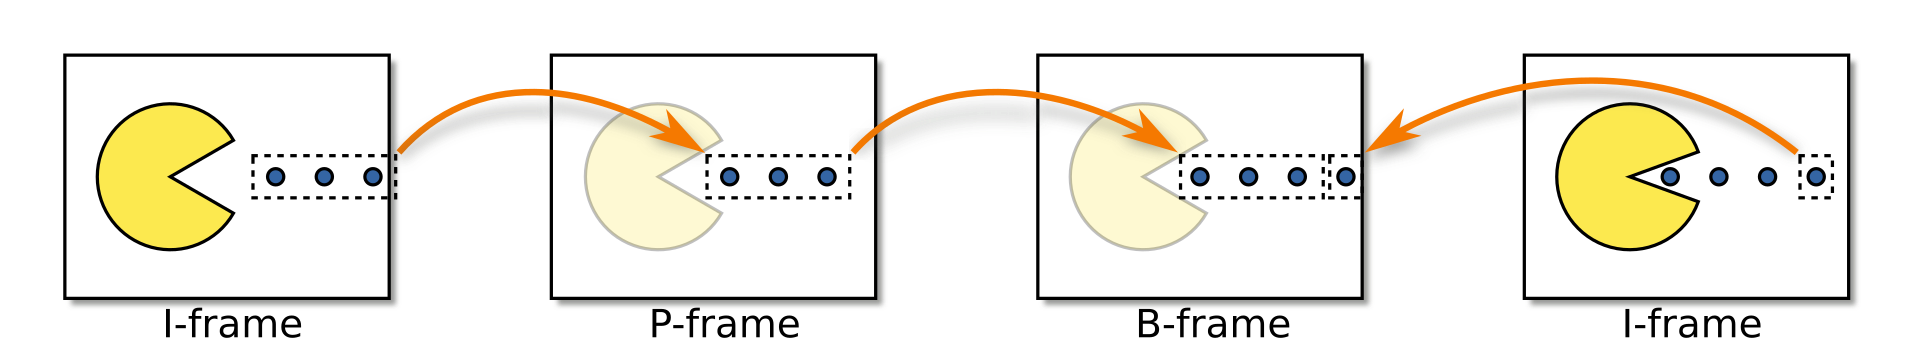
\includegraphics[width=1.0\linewidth]{chapter3/FIGS/compression.png}
    \begin{captext}
    \\[0.1cm] \small I frames are full frames which are interleaved with partial frames called P frames and B frames. These are frames that contain predicted motion based on previous frames and future frames within the transmission buffer.
    \end{captext}
    \caption{Video Compression Frame Types (Adapted from \cite{Wikipedia})}
    \label{fig:compression-demo}
\end{figure}

\begin{figure}
    \centering
    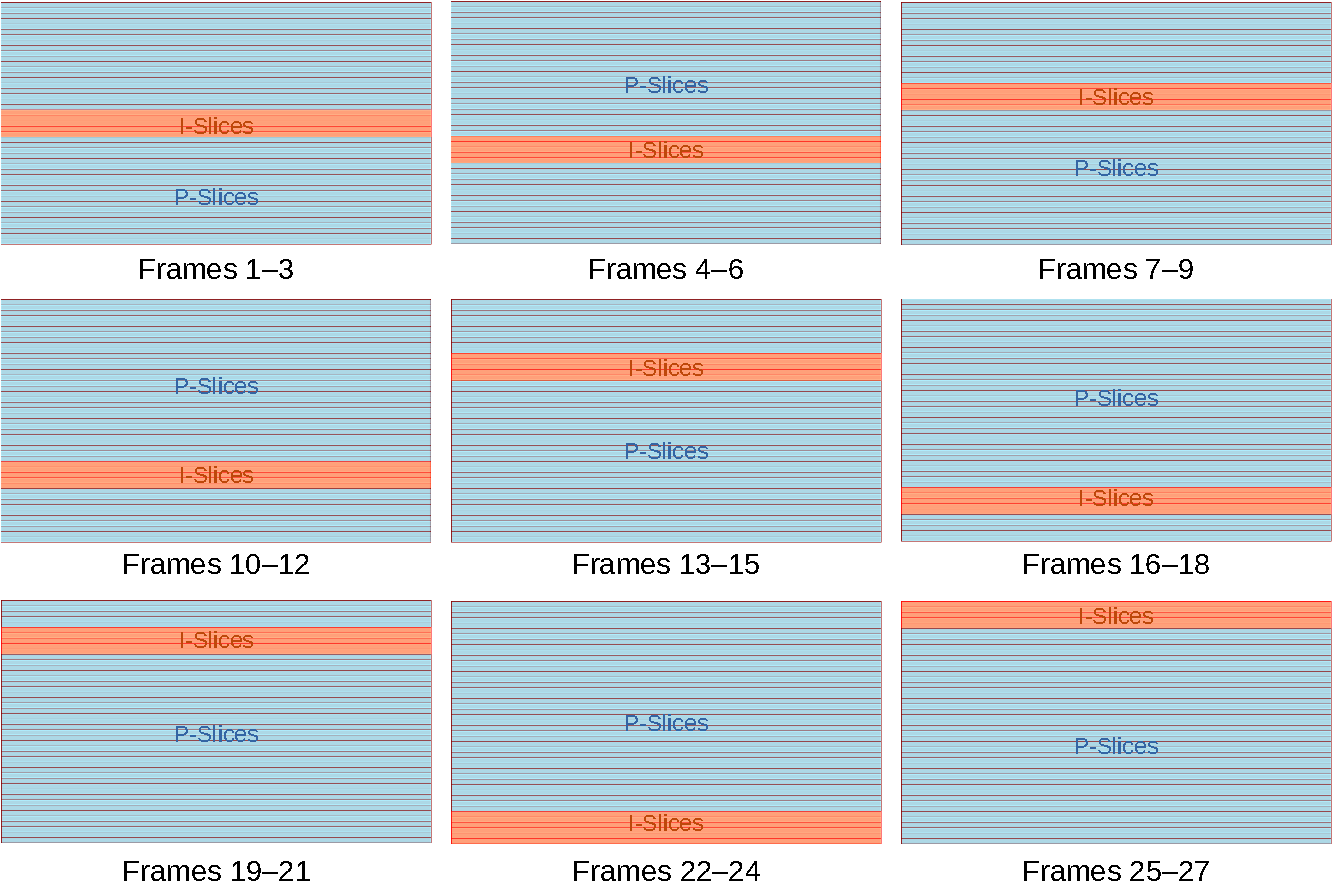
\includegraphics[width=0.9\linewidth]{chapter3/FIGS/slice-encoding-crop.pdf}
    \begin{captext}
    \\[0.1cm] \small Each segment of three frames contains one I-slice (shown in orange) and transmits the remaining slices as P-slices (shown in blue). The I-slice that is sent is chosen from the center of the frame going outward. After 30 frames, the process starts from the beginning.
    \end{captext}
    \caption{Intra-Refresh Slice-Decode Stream}
    \label{fig:slice-encoding}
\end{figure}

\section{Processing The Video Stream on the Watch}
There are two obvious methods for offloading the drone video stream from the watch to the edge. The first is to decode the drone stream on the watch and then ship the decoded frames to the edge. This allows the watch to throttle its send rate to account for 4G transmission overheating. The second is to directly offload the stream packets from the drone network to the cloudlet, where they can then be decoded. This involves the least amount of computation power on the watch, but requires a higher transmission rate. I will refer to these as decode-on-device and decode-on-edge respectively.

\subsection{Method 1: Decode-on-Device}
\label{sec:method-1}
Decode-on-device involves the watch decoding the drone video stream then sending decoded frames individually to the edge. This allows for some pre-processing on the watch side, such as downscaling or stream throttling for bandwidth saving. Unfortunately, the Anafi's intra-refresh slice-decode stream poses a major hurdle to this method's success: due to its construction, \textit{every frame must be decoded in order to maintain a coherent stream}. This is in stark contrast to a typical stream, which only requires the I frames (usually generated at around 1~fps) to be decoded to maintain coherence. As such, any device consuming the drone stream must decode one frame every 33~ms on average to keep up with the 30~fps output and prevent drifting latency, regardless of cellular transmission throughput. Drifting latency is a phenomenon where latency increases over time due to queueing delay. If a device drops packets to keep up with this strict time bound, it could cause some loss of quality as important I slices are discarded. On most devices, this is not an issue. But on the constrained compute of the Galaxy Watch 4, even relatively light workloads are considered difficult. Table~\ref{tab:decoding-time} shows the time taken to decode a frame of the Anafi's video stream by the watch, the Pixel 4a, and the Unihertz Jelly Pro. As shown, both the watch and the Jelly Pro cannot decode fast enough to maintain stable latency.

\begin{table}
        \centering
        \begin{tabular}{|l|c|}
                \hline
                & Decode Time \\
                \hline
                Samsung Galaxy Watch & \color{red}{55ms} \\
                Unihertz Jelly Pro & \color{red}{35ms} \\
                Google Pixel 4a & 25ms \\
                \hline
        \end{tabular}
        \begin{captext}
                \centering
                \\[0.1cm] \small \color{red}Red denotes a decode rate that is  too slow at 30~FPS.
        \end{captext}
        \caption{Average Decoding Time by Platform}
        \label{tab:decoding-time}
\end{table}

\begin{table}
\centering
\begin{tabular}{|r|c|c|}
\hline
Sleep&\multicolumn{2}{|c|}{Payload Size}\\
\cline{2-3}
Interval & 35~KB& 100~KB\\
\hline
33 ms & \redcross & \redcross \\
100 ms & \redcross & \redcross \\
500 ms & \redcross & \redcross \\
800 ms & \redcross & \redcross \\
1000 ms & \greencheck & \greencheck \\
\hline
\end{tabular}
\begin{captext}
\\[0.1cm]
\redcross\hspace{0.1in} thermal shutdown\\
\greencheck\hspace{0.1in} no thermal shutdown
\end{captext}
\caption{Effect of Sleeps}
\label{tab:thermal-sensitivity}
\end{table}

\subsection{Method 2: Decode-on-Edge}
\label{sec:method-2}
Decode-on-edge avoids decoding on device by directly sending the drone stream packets over cellular to the cloudlet, where they can then be decoded. With this method, computation on the device is minimal but network transmission is much more frequent. This is a good tradeoff in many cases, but on the watch, heavy transmission workloads may cause overheating. To determine the effect of transmission on the watch thermals, I devised a simple experiment: the watch sends a variable size packet, representing typical stream packet sizes (35KB up to 100KB), over the network with variable sleep times in between sends. There is no video stream or other onboard computation involved, only raw transmission. Table~\ref{tab:thermal-sensitivity} shows the results of this experiment. It is clear that the bottleneck on the watch is not the packet size but the send rate. Any send rate above 1~Hz causes thermal shutdown. This means that decode-on-edge streaming is mostly out of the question.

\begin{figure}
    \centering
    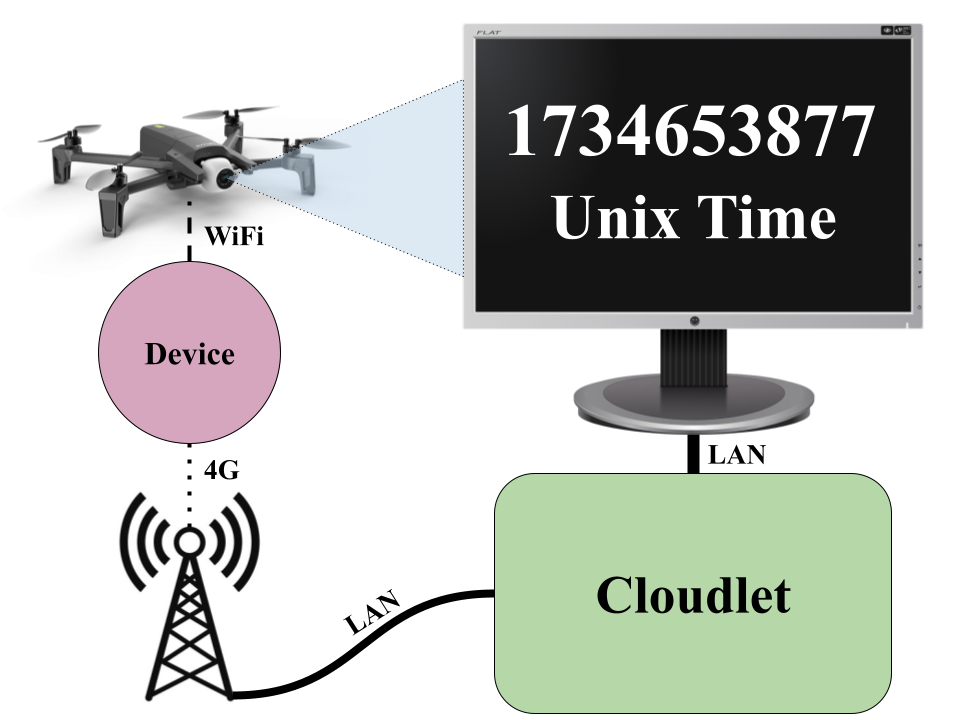
\includegraphics[width=0.75\linewidth]{chapter3/FIGS/mtp-experiment.png}
    \begin{captext}
    \\ \small The drone camera captures UNIX time displayed on a monitor that is connected to the cloudlet. It then sends the video stream over the device to the cloudlet. The total latency is the difference between the observed time in the stream versus the actual time the frame was received.
    \end{captext}
    \caption{Streaming Experiment}
    \label{fig:streaming-experiment}
\end{figure}

\section{The Quest for a Working Stream}
\label{sec:quest-working-stream}
A successful stream to the cloudlet must have acceptable latency, throughput, and image quality. Without these aspects, the stream will not be usable by AI algorithms running on the edge and therefore cannot contribute to fully-autonomous operation. Specifically, the stream must have:
\begin{itemize}
    \item \textbf{Sustainability}: the watch stream must sustain itself for the duration of a drone flight (at least 20 minutes).
    \item \textbf{Stable Latency}: the watch stream must process frames on average equal to or faster than 33~ms to keep up with the 30~fps stream from the drone.
    \item \textbf{High-Quality Frames}: the watch stream must deliver ``quality'' images to the cloudlet that lack significant visual artifacts and can thus be used by computer vision algorithms.
\end{itemize}
The austere environment on the watch makes achieving such a stream a challenge. The watch cannot decode frames fast enough to maintain stable latency, and thus cannot decode-on-device and send at a throttled framerate. It also cannot transmit consistently enough to decode-on-edge. To discover a path forward, I devised a set of experiments that would better characterize the bottlenecks in the system. By understanding these bottlenecks, an effective solution could be found.

\subsection{Experimental Setup}
\label{sec:streaming-experiment-setup}
For each of the following experiments, the setup is identical. The drone is started so that its RTSP stream and WiFi network are initialized. Then, the client device is connected to the drone’s WiFi network and the stream application is launched on the device. The application uses a variable method to stream image data from the drone to a cloudlet. When the frame arrives at the cloudlet, it is saved along with its time of arrival. The drone’s camera is pointed at a screen connected directly to the cloudlet which is displaying the current UNIX timestamp. This effectively timestamps each frame produced by the drone, a feature not present in the closed source stream hardware. By comparing the UNIX timestamp in the received image and its time of arrival, the transmission latency can be determined in post processing. The UNIX timestamp can also be used to determine the time at which thermal shutdown occurs. Figure~\ref{fig:streaming-experiment} shows the experimental setup. For experiment 1 and 2, I provide two other devices, the Google Pixel 4a and the Unihertz Jelly Pro as baselines. The duration of the experiments in all cases is the duration of a drone flight: 20 minutes.

\begin{table}
\centering
\begin{tabular}{|l|c|c|c|c|}
\hline
    & Pass- & Decode & Decode & Decode \\
    & Through & No & 3~fps & 1~fps \\
    & Stream & Throttle & Throttle & Throttle \\
\hline
Samsung Galaxy Watch 4 & \cellcolor{red!20}68~s & \cellcolor{red!20}380~s & \cellcolor{red!20}565~s & \cellcolor{green!20}DNO \\[0.1cm]
\hline
Unihertz Jelly Pro & \cellcolor{green!20}DNO & \cellcolor{red!20}TT & \cellcolor{red!20}TT & \cellcolor{green!20}DNO  \\[0.1cm]
\hline
Google Pixel 4a & \cellcolor{green!20}DNO & \cellcolor{green!20}DNO & \cellcolor{green!20}DNO & \cellcolor{green!20}DNO \\[0.1cm]
\hline
\end{tabular}
    \begin{captext}
    \\[0.1cm] \small Time in seconds before the device experiences a thermal shutdown. DNO means that the device did not overheat for the duration of the experiment (20~minutes). TT means that the device experienced thermal-related CPU throttling which affected performance.
    \end{captext}
\caption{Experiment 1: Sustainability}
\label{tab:time-before-overheating}
\end{table}

\subsection{Experiment 1: Sustainability}
\label{sec:exp1-sustainability}
In this experiment, I timed each device running either decode-on-device~\S\ref{sec:method-1} or decode-on-edge ~\S\ref{sec:method-2}. For the decode-on-device runs, I added additional tests with throttling. In these cases, the device decodes at the full frame rate but only sends to the cloudlet at the specified framerate. Table~\ref{tab:time-before-overheating} shows the results of the experiment. The watch clearly cannot sustain decode-on-edge streaming for any significant duration (about 1 minute), and can sustain non-throttled and 3~fps throttled streaming for up to 9 minutes.  However, the 1~fps throttled stream did not overheat for the duration of the test. This implicates 4G transmission as the main thermal bottleneck and sets an upper-bound for transmission frequency at 1~Hz. The Google Pixel 4a, unsurprisingly, breezed through all four tests. The Jelly Pro had trouble with the higher send rate of some decode-on-device tests but was overall good. This shows that slightly better thermals would drastically improve sustainable performance on the watch. 


\subsection{Experiment 2: Stable Latency}
In this experiment, I setup each device running the same methods as in Section~\ref{sec:exp1-sustainability}. This time, I measured the stream latency over the course of the test. Table~\ref{tab:stable-latency} shows the results of the experiment. No method provided a stream with stable latency on the watch. On the Jelly Pro, only the 1~fps throttled stream did. This implies that for the non-throttled and 3~fps throttled stream, the network transmission affected the decoding performance, slowing it down and causing latency to drift. On the Pixel 4a, all decode-on-device methods provided stable latency. No device successfully performed decode-on-edge streaming without drift. Clearly, a different approach is needed on the watch to guarantee consistent latency.

\begin{table}
\centering
\begin{tabular}{|l|c|c|c|c|}
\hline
    & Pass- & Decode & Decode & Decode \\
    & Through & No & 3~fps & 1~fps \\
    & Stream & Throttle & Throttle & Throttle \\
\hline
Samsung Galaxy Watch 4 & \cellcolor{red!20}DRIFT & \cellcolor{red!20}DRIFT & \cellcolor{red!20}DRIFT & \cellcolor{red!20}DRIFT \\[0.1cm]
\hline
Unihertz Jelly Pro & \cellcolor{red!20}DRIFT & \cellcolor{red!20}DRIFT & \cellcolor{red!20}DRIFT & \cellcolor{green!20}1~s  \\[0.1cm]
\hline
Google Pixel 4a & \cellcolor{red!20}DRIFT & \cellcolor{green!20}1~s & \cellcolor{green!20}1~s & \cellcolor{green!20}1~s \\[0.1cm]
\hline
\end{tabular}
    \begin{captext}
    \\[0.1cm] \small Latency in seconds. DRIFT means that the latency increased over the duration of the experiment (20~minutes).
    \end{captext}
\caption{Experiment 2: Stable Latency}
\label{tab:stable-latency}
\end{table}

\begin{table}
\centering
\begin{tabular}{|l|c|c|c|c|}
        \hline
        & $c = 1$ & $c = 2$ & $c = 3$ & $c = 4$ \\[0.1cm]
        \hline
$d = 1$ & 7~s, 80\% & 7~s, 80\%	& 8s, 90\%	& 8~s, 70\% \\[0.1cm]
\hline
$d = 2$ & 7~s, 80\% & 7~s, 80\% & 7~s, 90\%	& 7~s, 80\% \\[0.1cm]
\hline
$d = 3$ & 1~s, 30\% & \cellcolor{green!20}1~s, 99\%	& 4~s, 60\% & 4~s, 50\% \\[0.1cm]
\hline
$d = 4$ & $\leq$ 5\% & 1~s, 50\% &	1~s, 10\% & 6~s, 30\% \\[0.1cm]
\hline
\end{tabular}
    \begin{captext}
    \\[0.1cm] \small Latency in seconds followed by the approximate percentage of visual-artifact-free frames produced during the test. Combinations off the grid did not produce acceptable results, either due to drifting latency or poor quality. Visual quality is determined subjectively.
    \end{captext}
\caption{Experiment 3: High-Quality Frames}
\label{tab:hq-frames}
\end{table}

\subsection{Experiment 3: High-Quality Frames}
If the watch decodes the stream as outlined in~\S\ref{sec:method-1}, it produces very high-quality images with no visual artifacts at the cost of drifting latency. This is not acceptable by the standards outlined earlier in Section~\ref{sec:quest-working-stream}. Even so, room for compromise remains. While not desirable, intentional packet dropping of the video stream prior to decoding is an effective way to reduce latency at the cost of quality, since fewer stream packets reduces the time spent decoding. In this experiment, I determine how much packet dropping is acceptable to preserve quality. I test the watch under the 1~fps throttled decode-on-device workload, decoding chunks of $c$ packets and then subsequently dropping $d$ packets. For example, a $c=2, d=2$ scheme would involve decoding 2 out of every 4 packets. Table~\ref{tab:hq-frames} shows the results of the experiment. As $d$ increases, quality drops but latency decreases as the average time to decode shrinks. In the other direction, as $c$ increases, latency generally increases too since the average time to decode grows. At $c=2, d=3$, there is a sweet-spot where the watch latency is minimal and the impact on frame quality is also minimal. It is this combination that finally produces a workable stream.

\begin{figure}
    \centering
    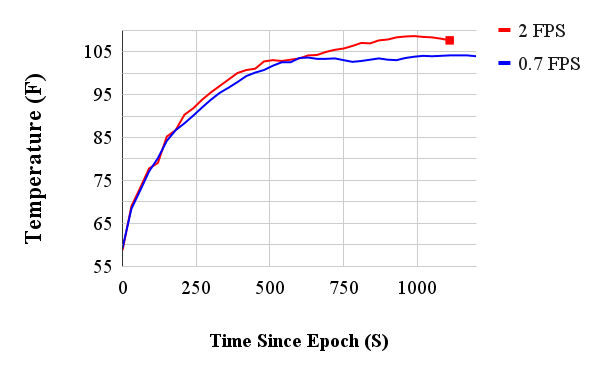
\includegraphics[width=0.8\linewidth]{chapter3/FIGS/temperature.png}
    \begin{captext}
    \\[0.1cm]
    \small The red square at the end of the 2~fps temperature curve indicates a thermal shutdown occurred. The 0.7~fps graph continues without overheating.
    \end{captext}
    \caption{Watch Temperature at Different Throttling Levels}
    \label{fig:temperature}
\end{figure}

\subsection{The Stream in Practice}
\label{sec:stream-in-practice}
Putting together the results of the three experiments, a working solution emerges. It solves each of the requirements presented in Section~\ref{sec:quest-working-stream}:
\begin{itemize}
    \item \textbf{Sustainability}: \textit{the watch stream must sustain itself for the duration of a drone flight (at least 20 minutes).}
    The watch throttles sending frames to the cloudlet to 1~Hz which is sustainable for 20 minutes.
    \item \textbf{Stable Latency}: \textit{the watch stream must process frames on average equal to or faster than 33~ms to keep up with the 30~fps stream from the drone.}
    The watch drops 3 packets for every 2 it decodes which reduces the average decode time enough to keep up with the drone stream.
    \item \textbf{High-Quality Frames}: \textit{the watch stream must deliver ``quality'' images to the cloudlet that lack significant visual artifacts and can thus be used by computer vision algorithms.}
    The watch decodes enough packets to maintain a high-quality stream.
\end{itemize}
Integrated into the larger application, parts of this streaming scheme must be modified to make way for other compute resources. In particular, throttling to 1~fps proves too demanding once other processes are factored in. Once throttling is dropped to 0.7~fps, the stream once again is functional. Figure~\ref{fig:temperature} shows the watch temperature over time with a 2~fps and a 0.7~fps throttled stream within the larger application. At 2~fps, the stream experiences thermal shutdown once the watch reaches an external temperature of 108\degree F. At 0.7~fps, the watch maintains an external temperature under 105\degree F for 20 minutes without ever experiencing a thermal shutdown.

\section{Summary}
The core insight of SteelEagle is that heavy onboard compute can be avoided by offloading computation from drones over a cellular network to a cloudlet. As a first demonstration of this concept, I successfully connected the Parrot Anafi to a cloudlet via the Galaxy Watch 4. The watch, despite its thermal constraints, can offload the drone's video stream over 4G at 0.7~fps with 1~s latency while simultaneously sending actuation commands. The drone can also operate BVLOS without the need for any connected human pilots. Now, all that is needed is a complementary edge software backend that can provide the drone with the intelligence required for full autonomy.

\chapter{The SteelEagle Backend}
Fully-autonomous drones are only as effective as the artificial intelligence software and decision-making protocols they use. SteelEagle is no different; its performance is tightly correlated with the sensor processing and control algorithms running on the edge. However, its offload-based design poses additional constraints: all sensor data from the drone is inherently latent and may have suboptimal throughput. Furthermore, cloudlets may be required to serve multiple drones, and may have to deal with changing network conditions that hamper bandwidth.

In this chapter, I will discuss my architecture for the SteelEagle backend. I will show how it addresses these unique problems and how it adapts to its network environment. In Section~\ref{sec:remote-intelligence-framework}, I outline the overall design of the system and its interaction with drone clients. In Section~\ref{sec:eval}, I evaluate the system on a few basic tasks to understand its capabilities.

\section{An Edge Intelligence Framework for Drones}
\label{sec:remote-intelligence-framework}
The SteelEagle backend is made up of three main modules: compute, command and control, and storage. To handle transmission between these modules and between the cloudlet and external clients, traffic is split into two channels, the data plane and the control plane. Each channel uses a different communication protocol to suit their specific quality-of-service demands. Figure~\ref{fig:sys-arch} shows the full system architecture. The overall system is characterized by two main data flows: the remote processing flow through the data plane and the remote control flow through the control plane. I will outline both to illustrate how the system operates.

\begin{figure}
    \centering
    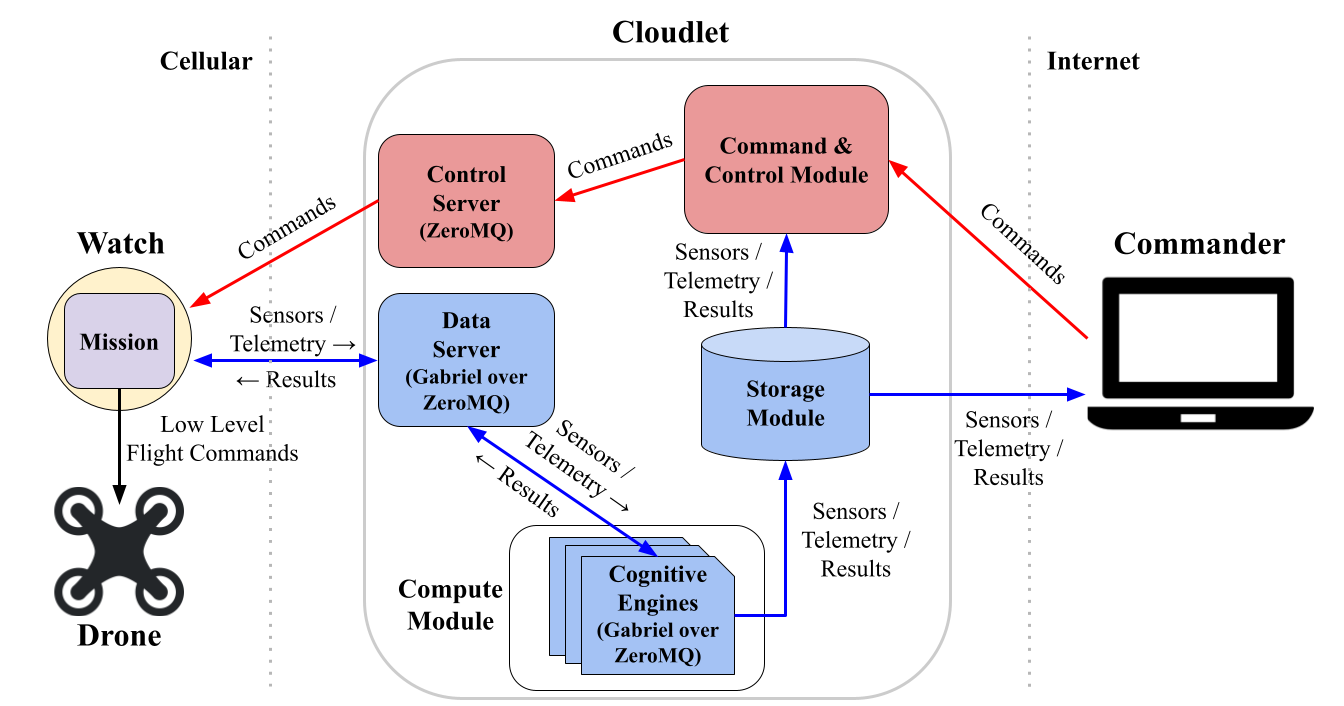
\includegraphics[width=0.9\linewidth]{chapter4/FIGS/arch.png}
    \begin{captext}
    \\[0.1cm]
    \small The remote processing flow, which handles the processing of the drone's sensor stream and the delivery of generated results, is highlighted in blue. The remote control flow, which delivers all commander messages and auto-generated commands from the command and control module, is highlighted in red.
    \end{captext}
    \caption{SteelEagle System Architecture}
    \label{fig:sys-arch}
\end{figure}

\begin{figure}
    \centering
    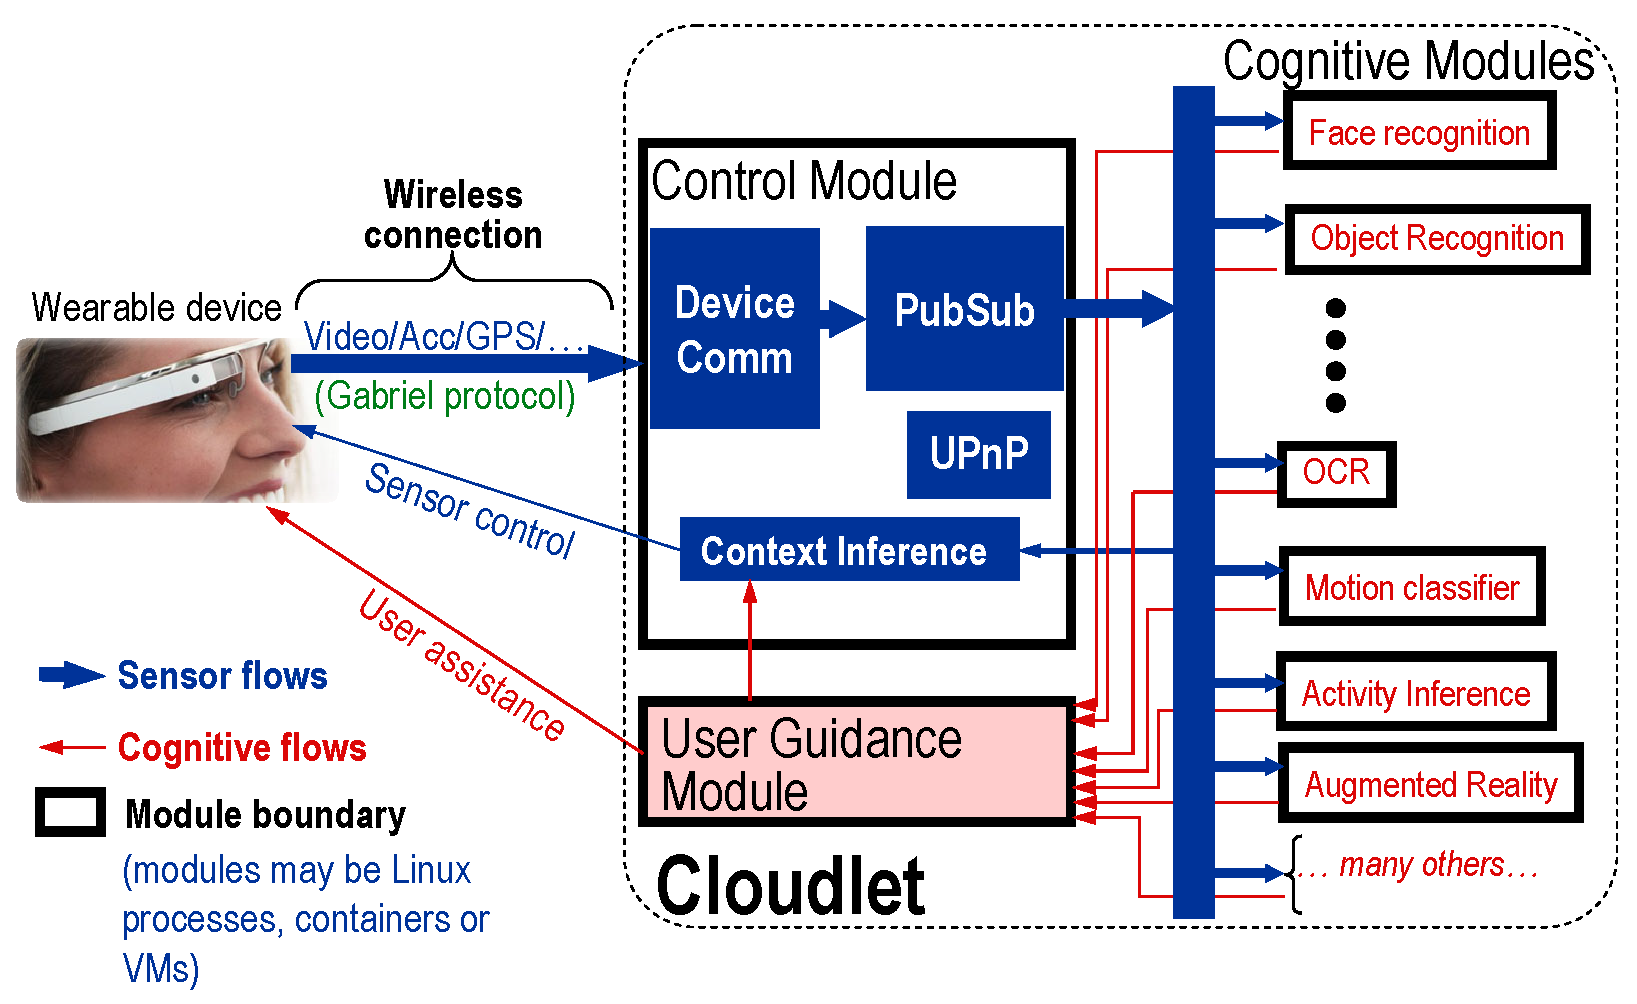
\includegraphics[width=0.8\linewidth]{chapter4/FIGS/gabriel.png}
    \begin{captext}
    \\[0.1cm]
    \small In the case of SteelEagle, the Wearable Device is replaced with a drone communicating over cellular. The User Guidance VM not only sends processing results back to the drone through the data server (as shown in Figure~\ref{fig:sys-arch}), but also stores results in the storage module.
    \end{captext}
    \caption{Gabirel Cognitive Assistance Model (Adapted from ~\cite{Ha2014})}
    \label{fig:gabriel-cognitive-assistance}
\end{figure}


\subsection{Remote Processing Flow}
Perhaps the most important data flow in SteelEagle is the remote processing flow, outlined in blue in Figure~\ref{fig:sys-arch}. The role of this flow is straightforward: retrieve sensor data and telemetry from the drone, run the requested algorithm by the current mission, return results to relevant clients, repeat. Yet there are additional considerations that complicate this seemingly simple picture. First, bandwidth is a precious resource for mobile systems, and availability may vary highly based on current network conditions~\cite{Forman1994}. For this reason, it is important that the stream retrieval portion of the data flow can cope with bandwidth constriction without introducing too much latency. Second, many DNNs require vast computational resources to run quickly. Some may not be able to sustain sufficient throughput to keep up with the drone's stream. If the data flow takes on multiple tenants without adapting its inference rate to model throughput, it could lead to queueing delay and thus added latency.

\subsubsection{Gabriel and the Cognitive Assistance Model}
To address both of these problems, the SteelEagle remote processing flow leverages the Gabriel Cognitive Assistance model~\cite{Ha2014}. Proposed in 2014, Gabriel is a bandwidth-adaptive edge intelligence system that provides near real-time sensor processing results to mobile clients (Figure~\ref{fig:gabriel-cognitive-assistance}). Gabriel is bandwidth-adaptive and model-throughput-adaptive thanks to its token-based flow control protocol. Token-based flow control is a technique for avoiding queueing delay in a client-producer server-consumer system using data objects called tokens. Tokens are a certificate that signal the server or client to act; if the server has a token, it has client data that needs to be processed and if the client has a token, it must send its most recently produced data to the server. 

At system start, a set number of tokens is agreed upon between the server (also called the control VM in Figure~\ref{fig:gabriel-cognitive-assistance}) and client. The server and client exchange these tokens based on their individual processing rates. For instance, if the client's send rate outpaces the server's processing rate, the server will be in possession of a large share of the tokens and vice versa. If no tokens remain on the client side, the client drops the current payload until it sees a new token. If no tokens remain on the server side, it waits to receive new client data. In this model, the client only ever sends the most recently produced payload which prevents the server from receiving highly latent data.

In Gabriel, each distinct sensor processing algorithm is called a ``cognitive engine''. Gabriel supports running several cognitive engines simultaneously, and manages their input data queues. Each cognitive engine is run in a separate container on the host machine, and is shipped data via an inter-process communication channel. Gabriel's tokens are shared among the engines which effectively bottlenecks the client send rate to the throughput of the fastest engine. On slower engines, queued data is dropped to ensure the latest data available is processed.

\subsubsection{SteelEagle Upgrades to Gabriel}
Gabriel is designed for mobile clients that have stable connections to the edge over WiFi. Due to this, underlying connections are made via websockets. Websockets are a point-to-point connection medium that are intended for web browser to server links. They are performant but must be modified to properly deal with disconnections. In the case of SteelEagle,  cellular links to the backend can be easily disrupted by drone motion or interference. This renders websockets sub-optimal. To fix this, SteelEagle replaces the underlying communication in Gabriel with ZeroMQ sockets that provide auto-reconnection among other quality-of-service guarantees~\cite{ZeroMQ}. Other connections within SteelEagle that are not Gabriel-regulated use pure ZeroMQ sockets (Figure~\ref{fig:sys-arch}).

Within SteelEagle, the Gabriel control VM is called the \textit{data server} and cognitive engines are managed by an entity called the \textit{compute module} (see Figure~\ref{fig:sys-arch}). In most cases, the compute module will spawn a pre-specified set of algorithms demanded by a drone mission at mission start. In the future, I envision that it may also support runtime addition and deletion of cognitive engines and dynamic scale-out at runtime to adapt to constrained computation resources or new mission parameters.

Unlike the default Gabriel implementation, SteelEagle supports multiple consumer clients of processing results (generated by the User Guidance VM in Figure~\ref{fig:gabriel-cognitive-assistance}). The main consumer of these results other than the drone is the storage module (see Figure~\ref{fig:sys-arch}). The storage module is a database responsible for logging all processed results in addition to the raw sensor and telemetry sent by the drone. This can be read by other monitoring clients such as the command and control module if needed for orchestration purposes.

\subsubsection{Supported Cognitive Engines}
As a result of its Gabriel-based design, SteelEagle supports a wide range of cognitive engines. To add new engines, users simply need to work within the Gabriel cognitive engine interface and connect to the Gabriel server~\cite{Ha2014}. The server will automatically configure the requested type of sensor stream and manage timely delivery of data to the engine. For initial evaluation purposes, I have configured two engines useful for drone operations: object detection and obstacle avoidance. I will detail their implementation in Section~\ref{sec:eval}.

\subsection{Remote Control Flow}
The remote control flow handles interactions between humans and SteelEagle drones. Within the SteelEagle ecosystem, since the drones are fully-autonomous, there are no conventional human pilots. Instead, humans who interact with SteelEagle drones are referred to as ``commanders''. Commanders create missions, send missions to aircraft, and monitor telemetry data to ensure continued safe operation. They also have the ability to manually pilot a connected aircraft in case of emergency. Figure~\ref{fig:commander} shows the commander UI. It provides continuous feedback on the progress of the mission on a map.  It also displays live sensor streams, including video, transmitted by the drone. It includes several buttons to upload missions, take manual control of one or more aircraft, and order one or more aircraft to return home.

Messages sent by commanders are aggregated in the command and control module (see Figure~\ref{fig:sys-arch}). Here, messages are relayed to the control server which then sends them to the target aircraft over a direct, unregulated socket connection. This is in contrast to the data server, which uses token-based flow control socket connections. The reason for this difference is that messages sent by commanders, especially emergency commands, are deemed to be high priority and must therefore be forced over the link as quickly as possible without any regard for bandwidth.

The command and control module also acts as an air traffic controller. That is, it manages the airspace inhabited by connected aircraft to ensure there are no mid-air collisions. For instance, it allocates non-intersecting altitude slices to different drones operating in the same mission area to ensure they are flying at different altitudes. The command and control module maintains up-to-date telemetry from all connected drone clients via the storage module and can therefore detect potential crashes before they happen.

\begin{figure}
    \centering
    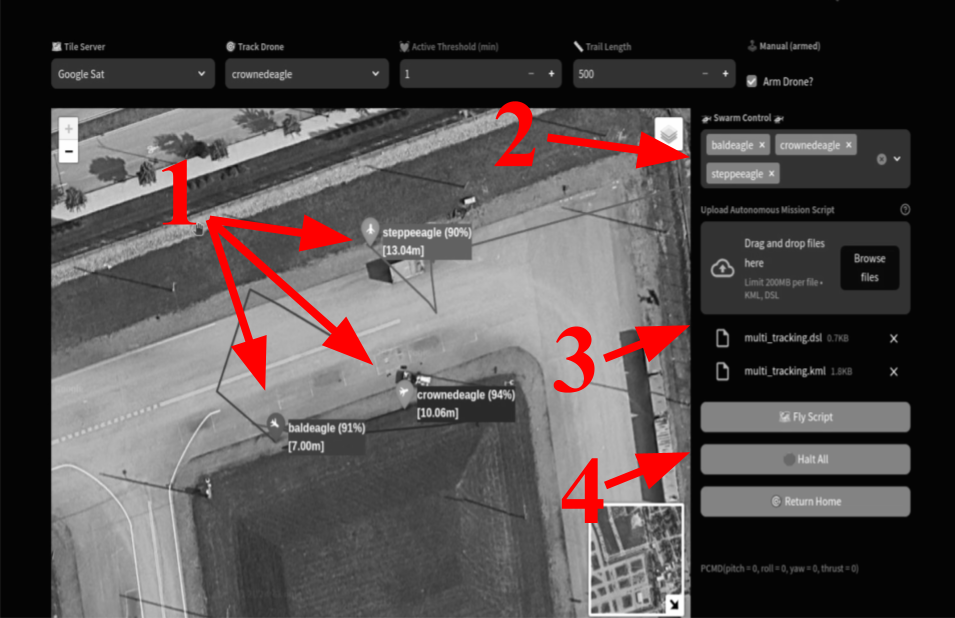
\includegraphics[width=1.0\linewidth]{chapter4/FIGS/commander.png}
    \begin{captext}
    \small \textit{\textbf{1.} Active drones with displayed battery percentage, altitude, and GPS location, \textbf{2.} Selection of command recipients, \textbf{3.} Mission upload tool, \textbf{4.} Emergency and manual command buttons}
    \end{captext}
    \caption{Commander Interface}
    \label{fig:commander}
\end{figure}

\subsubsection{Drone Missions}
Prior to flight, a mission is planned using a toolchain that starts with Google MyMaps. The flight route can be specified using waypoints, line segments and polygons. Actions such as capturing images, tracking particular objects, or avoiding obstacles can be associated with parts of the route, and can be linked together to form a primitive behavior tree. Behavior trees are a common way of expressing missions in a variety of robotics settings~\cite{Ghouzli2023}. An offline compilation step, usually performed on a commander computer, transforms the high-level specification into low-level drone-specific runtime actions on the cloudlet and on the drone.  In the case of the Parrot Anafi-Galaxy Watch 4 prototype, the compiler output is expressed via Ground SDK API Java classes and packaged into an Android DEX file. A drone simulator can be used for testing and visualization of this output. 

In its current form, SteelEagle assumes a one-to-one correspondence of drones and missions. In particular, each drone executes its given mission in isolation, without cooperation. In future, to support swarm operations, this would change. For now, this simple abstraction provides enough for basic autonomous drone operations.


\section{Evaluation}
\label{sec:eval}

Given the prototype constraints discussed in Section~\ref{sec:austere-computing} and my proposed backend architecture, I ask the following question: 
{\em ``Can my flight platform, with severe constraints on both local compute and edge offload, achieve autonomy for active vision?''} Recall, active vision tasks are those that require the drone to react in real time to its surroundings~\cite{Aloimonos1988, Ognibene2013}. To answer this question, I conduct experiments with a series of tasks of increasing difficulty that probe and quantify the limits of my flight platform:

\begin{itemize}

\item{{\bf Task-1:} Detecting a moving object while hovering.}

\item{{\bf Task-2:} Detecting and tracking an object by yawing to keep it in
    the field of view (FOV) as it moves.}

\item{{\bf Task-3:} Detecting and tracking an object by following it at a
    fixed leash distance as the object moves.}

\item{{\bf Task-4:} Detecting a moving object from high altitude, and
    then descending to closely inspect it.  }

\item{{\bf Task-5:} Detecting and avoiding static obstacles.}

\end{itemize}

My goal is to perform these tasks from takeoff to landing with no
human intervention.  Where possible, I test my
system against the Parrot Anafi Ai, a semi-autonomous COTS drone with LTE support, limited onboard tracking and obstacle avoidance.  It weighs more
than twice as much as my flight platform, and costs over five times as much~(Figure~\ref{fig:featurematrix}).  A less-constrained platform
can clearly do more, but it may weigh more too.  My focus is on
whether my 360~g drone-watch platform is too weak or just enough.

The cloudlet used in the following experiments has 36 CPU cores, 128~GB of RAM and an NVIDIA GeForce GTX 1080
Ti GPU.  It is capable of using a private CBRS LTE network for low end-to-end latency. However, since the Galaxy Watch is not able to connect over CBRS, all presented results are based on public cellular network infrastructure.

\subsection{Flight Duration}
\label{sec:flightduration}

Since my platform consists of mounting external components on an
existing drone, a reduction in flight duration is expected. This
reduction is important to quantify, as it directly impacts my
platform's range and practicality. In Figure~\ref{fig:battery}, I
show the hover time of the Parrot Anafi with a 0~g, 40~g, and 60~g
payload weight. The Galaxy Watch with harness is around a 40~g
payload. It is clear that the watch payload reduces battery life by $10\%$ to $20\%$ on average.

\begin{table}
	\centering
	\begin{tabular}{|l|c|c|c|}
		\hline
		& My Platform & Base Parrot Anafi & Parrot Anafi Ai \\
		\hline
		Cost & \$769 & \$469 & \$4,500 \\
		\hline
		Weight & 360~g & 320~g & 898~g \\ 
		\hline
		Detection & \cellcolor{green!30}Yes & \cellcolor{red!30}No & \cellcolor{red!30}No \\
		\hline
		Tracking & \cellcolor{green!30}Yes & \cellcolor{yellow!30}Yes* & \cellcolor{yellow!30}Yes*\\
		\hline
		Avoidance & \cellcolor{green!30}Yes & \cellcolor{red!30}No & \cellcolor{green!30}Yes\\
		\hline
		Programmable & \cellcolor{green!30}Yes & \cellcolor{green!30}Yes & \cellcolor{green!30}Yes\\
		\hline
		4G/5G & \cellcolor{green!30}Yes & \cellcolor{red!30}No & \cellcolor{green!30}Yes\\
		\hline
	\end{tabular}
	\begin{captext}
            \\[0.1cm]
		\centering
		\small *~Requires assistance from the pilot for initial object detection.
	\end{captext}
	\caption{Flight Platforms Relevant to my Experiments}
	\label{fig:featurematrix}
\end{table}

\begin{table}
\centering
\begin{tabular}{|l|c|c|c|c|c|c|}
\hline
&0~g &40~g &\cellcolor[HTML]{FF9470}\% Reduction 
 &60~g &\cellcolor[HTML]{FF9470}\% Reduction \\
 \hline
Battery 1 & 21:04 & 18:43 &11.16\% & 17:18 &17.88\% \\
 \hline
Battery 2 & 22:54 & 19:35 &14.48\% & 18:57 &17.25\% \\
 \hline
Battery 3 & 17:57 & 14:23 &19.87\% & 13:00 &27.58\% \\
 \hline
Battery 4 & 20:00 & 16:43 &16.42\% & 15:12 &24.00\% \\
 \hline
\end{tabular}
\caption{Flight Duration by Payload Weight}
\label{fig:battery}
\end{table}

\subsection{Event-to-Detection Latency}
\label{sec:event-to-detection-latency}

The agility of my system is limited by the end-to-end latency of the
processing pipeline~(Figure~\ref{fig:sys-arch}).  Events closer in
time than this limit may not be resolvable.  For example, a
surveillance target with a jerky motion will be perceived as moving
more smoothly.  Large, but brief, deviations from the smoothed path
may not be detected.  The larger the end-to-end latency, the greater
the need for predictive approaches in tracking fast-moving
targets.  This, in turn, leads to greater likelihood of errors due
to mis-prediction.

The base end-to-end latency of the pipeline can by replicating the experiment described in Section~\ref{sec:streaming-experiment-setup} and Figure~\ref{fig:streaming-experiment}. The
drone is kept stationary in a lab setting, with its camera pointing at a display attached to the cloudlet. Except
for the fact that the drone is not flying, everything else (hardware, software, and network) is identical to Figure~\ref{fig:sys-arch}.  The cloudlet-connected display shows the current time at millisecond
granularity.  An image of this timestamp is captured by the drone's camera, transmitted downstream, and recovered at the end of the pipeline.  Its difference from current time at recovery gives the end-to-end latency.  Figure~\ref{fig:e2elatency} presents my results from 30 samples. The distribution is heavy-tailed, with a mean of 1138~ms and a standard deviation of 157~ms.  The high mean and variability arise from jitter in LTE transmission, as well as from processing and scheduling delays on the drone, watch, and cloudlet.


\begin{figure}
\centering
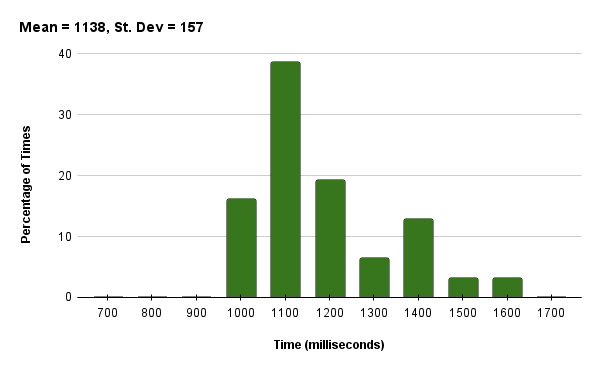
\includegraphics[width=0.7\linewidth]{chapter4/FIGS/new_mtp_watch.png}
\caption{Distribution of Detection Latency (Galaxy Watch)}
\label{fig:e2elatency}
\end{figure}


\subsection{Task-1: Object Detection While Hovering}
\label{sec:task1}

\subsubsection{Task Description}
\label{sec:task1-desc}

The accuracy of the computer vision pipeline complements its speed.
\begingroup
\setlength{\columnsep}{4pt}
Both are important for active vision.  A simple test is the detection
of a target on the ground when it moves into the camera's FOV.  The
problem is harder from higher altitude because objects are smaller and
DNNs perform poorly on objects that are just a few pixels in
size~\cite{Huang2017}.
Figure~\ref{fig:robomaster} shows the DJI Robomaster S1
robot~\cite{Robomaster2022} used as the detection target in my
experiments.  It is roughly the size of a small dog, and can be
remote-controlled over WiFi by a human driver.  It can also be
programmed to follow a predefined route, with speed variation in
different route segments. 

\begin{figure}
\centering
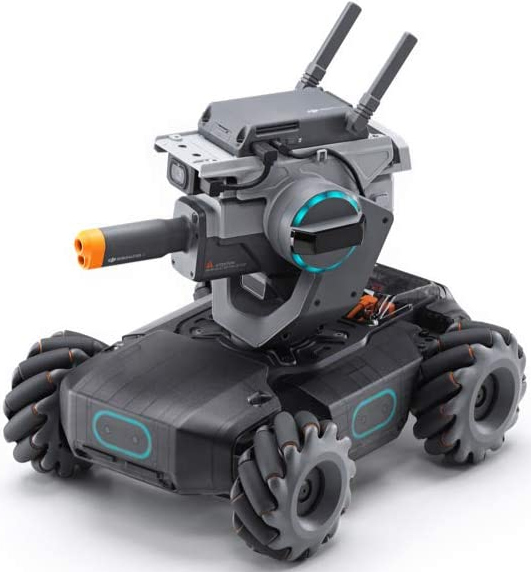
\includegraphics[width=0.4\linewidth]{chapter4/FIGS/robomaster.jpg}\\
{\footnotesize 432~x~330~x~304~mm\\[-0.05in]
\noindent(17~x~13~x~12~in)}
\caption{COTS Target}
\label{fig:robomaster}
\end{figure}

For Task-1, the robot is manually operated
on a freeform path that overlaps the FOV of the drone that is hovering
at fixed altitude.  In postprocessing, I compare ground truth~(GT) on
each processed frame with the output of the processing pipeline.  The
object detection DNN was created via transfer learning from
SSD-ResNet50~\cite{SSDResnet50} pre-trained on the COCO dataset.  The
training set was created from drone-captured images of the target
shown in Figure~\ref{fig:robomaster}.

\endgroup


\subsubsection{Results}
\label{sec:task1-results}

I perform this experiment at altitudes of 5~m, 10~m, and 15~m.
Accuracy is high at 5~m; a typical result is
Figure~\ref{fig:task1-images}(a), where the bounding box indicates
detection followed by correct target classification at high
confidence~(0.98).  The person at the top right and the distractor
object at the top middle are correctly ignored.  At 10~m, accuracy is
slightly lower.  An example of an erroneous result at 10~m is
Figure~\ref{fig:task1-images}(b), which shows a true positive~(TP)
(the target) at confidence 0.95 at bottom center, and a false
positive~(FP) (a person misclassified as the target at confidence
0.82) at center left.  At 15~m, accuracy suffers significantly.  An
example of an error at 15~m is Figure~\ref{fig:task1-images}(c).  This
shows an FP at center right (a person misclassified as the
target at confidence 0.86), and also a false negative~(FN) (missed target)
at center left.  Altitudes of 15~m and higher are clearly challenging
for this combination of target size, optical system, and processing pipeline.

\begin{figure}
\centering\small
\centering
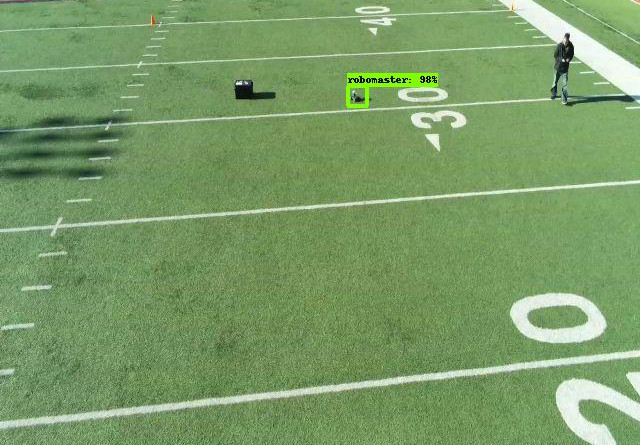
\includegraphics[width=0.6\linewidth]{chapter4/FIGS/fig-static-detection-example2-5m.jpg}\\
(a) Altitude = 5m\\[0.1in]
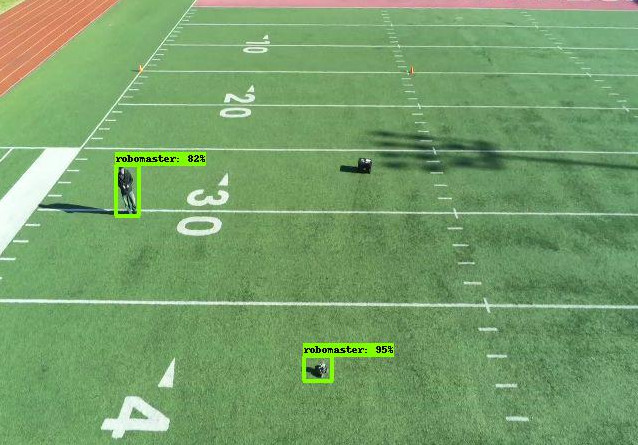
\includegraphics[width=0.6\linewidth]{chapter4/FIGS/fig-static-detection-example2-10m.jpg}\\
(b) Altitude = 10m\\[0.1in]
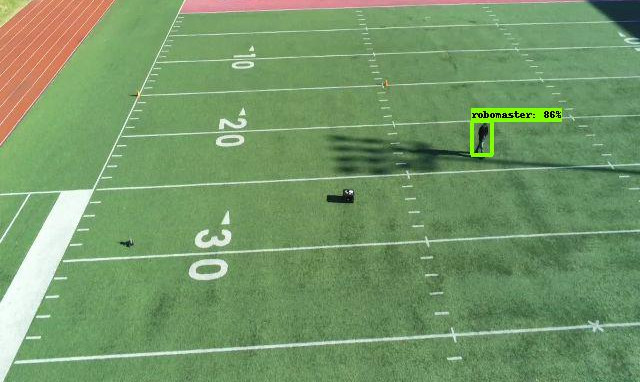
\includegraphics[width=0.6\linewidth]{chapter4/FIGS/fig-static-detection-example2-15m.jpg}\\
(c) Altitude = 15m
\caption{Task-1 Images}
\label{fig:task1-images}
\end{figure}

Table~\ref{tab:task1-results}~(a) shows the confusion matrix for
Task-1 at a confidence threshold of 0.7.  The scoring of images used
in this matrix requires explanation. Classic measures of precision and
recall address scene classification, where an entire image is
correctly or incorrectly classified.  In contrast, my setting
involves object detection.  It is possible for a single image to have
both a FP and a TP or FN.  Figure~\ref{fig:task1-images}(a) contains
a single TP, and no errors.  This is scored as a TP in the confusion
matrix.  Figure~\ref{fig:task1-images}(b) contains both a TP and an
FP; this is scored as an FP since errors trump correctness.  When
there are multiple errors, the worst error determines the score.
Figure~\ref{fig:task1-images}(c), for example, contains both an FP and
an FN.  I view FNs (hurting recall) as more serious errors than FPs
(hurting precision), and therefore score the whole image as an FN.
These rules preserve the invariant
$$GT_P + GT_N = TP + TN + FP + FN$$
where $GT_P$ and $GT_N$ refer to ground truth positives and negatives,
and TN refers to true negatives (no target in image).

\begin{table}
\centering\small
\begin{minipage}[b]{2.4in}
\centering\small
\begin{tabular}{|c|c|c|c|c|}
\hline
Alti-&\multicolumn{2}{c|}{Ground}&\multicolumn{2}{c|}{Detected}\\
\cline{4-5}
tude&\multicolumn{2}{c|}{Truth}& Pos& Neg.\\
\hline
5 m & Pos. & 85 & 71 & 13\\
    & Neg. &  0 & 1  & 0\\
\hline
10 m & Pos. & 90 & 55 & 30\\
     & Neg. &  0 & 5  & 0 \\
\hline
15 m & Pos. & 85 & 24 & 48 \\
     & Neg. &  0 & 13 & 0\\
\hline
\end{tabular}\\[0.05in]
{\footnotesize Threshold = 0.7}\\
(a) Detection Results\\
\end{minipage}
\begin{minipage}[b]{1.4in}
\centering
\begin{tabular}{|c|c|c|}
\hline
Alti-& Prec- & Re-\\
tude & ision & call\\
\hline
5 m & 0.99 & 0.85 \\
10 m &0.92 & 0.65\\
15 m & 0.65 & 0.33 \\
\hline
\end{tabular}\\[0.05in]
(b) Precision and Recall
\end{minipage}

\caption{Task-1 Results}
\label{tab:task1-results}
\vspace{-0.2in}
\end{table}


At 5~m, a total of 85 frames are processed.  The column labeled
``Ground Truth'' shows that all 85 contain a target instance.  The
``Detected'' columns show that 71 out of the 85 are correctly detected
and classified~(TPs), but 13 are missed~(FNs).  At 10~m, all 90
processed frames contain an instance of the target, but only 55 of
them are correctly detected~(TPs).  There are 30~FNs and 5~FPs.  At
15~m, accuracy suffers considerably.  Out of 85 total processed
frames, all are GT-positive.  However, only 24 of them are correctly
detected~(TPs).  There are 48~FNs and 13~FPs.
Table~\ref{tab:task1-results}~(b) shows the precision and recall
resulting from these detection results.  These values are excellent at
5~m.  Recall is noticeably degraded at 10~m.  Both precision and
recall suffer at 15~m.  These results suggest the importance of active
vision. Dropping to a lower altitude could confirm
or refute the sighting of an object from higher altitude. 

\subsection{Task-2: Keeping Sight of  a Moving Object}
\label{sec:task2}

\subsubsection{Task Description}
\label{sec:task2-desc}

Processing a frame in Task-1 does not lead to actuation of the drone.
In contrast, Task-2 represents a simple form of active vision. After
detecting a moving target, the drone yaws to keep the target visible
in the frame. There is no forward or backward motion, only rotation to
keep the object in the FOV. To find the target in frame,  Target speed and motion predictability
clearly influence this task.  A fast-moving target that unpredictably
and frequently changes its path is clearly hard to track.  As
discussed earlier~(\S~\ref{sec:event-to-detection-latency}), the end-to-end latency of
processing constrains tracking agility. With the help of the pilot
(using the FreeFlight app), the Anafi Ai can also perform this task
and thus I use it as a benchmark for my platform.

\begingroup
\setlength{\columnsep}{4pt}
\begin{figure}
\centering
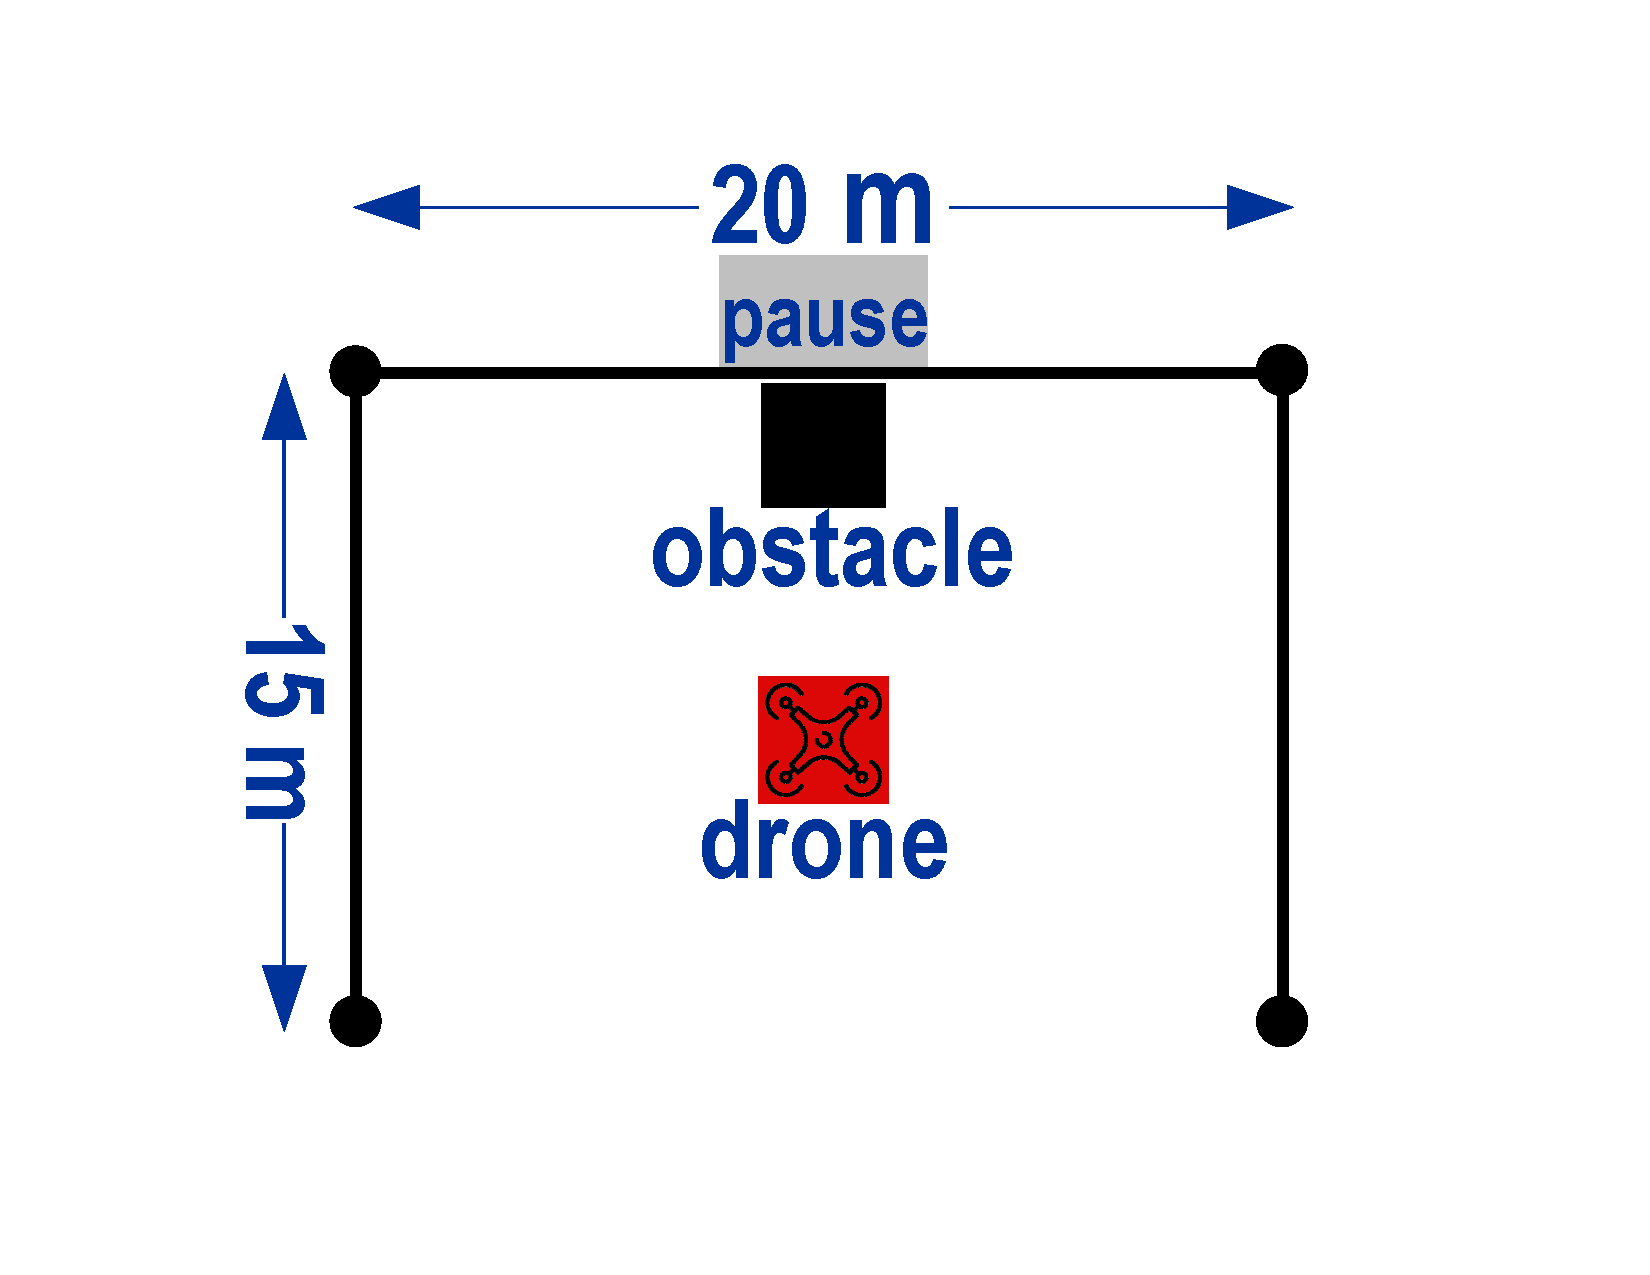
\includegraphics[width=0.4\linewidth]{chapter4/FIGS/fig-yaw-ushape.pdf}\\
\caption{Target Occlusion}
\label{fig:yaw}
\end{figure}

As shown in Figure~\ref{fig:yaw}, I set up a rectangular
(approximately 20~m~x~15~m) course marked by 4 cones.  The drone is
placed near the center of the rectangle and takes off to a fixed
altitude of 2 meters. A 2~m tall by 0.5~m wide foam pillar is placed
to occlude the target along the center of the back edge. For each run,
the target moves along the right, back, and left edges in a u-shape
two times. To test the ability of each platform to reacquire lost
targets, I vary the time spent being occluded, starting with no
pause, then pausing for 2 seconds behind the pillar, and finally a 5
second pause. Three runs of each delay were recorded.  For the Anafi
Ai, the pilot must draw a bounding box around the target in order to
start tracking; my platform automatically acquires and re-acquires
the target.  Since my platform is constrained to below 1~fps, we
compare results from the two platforms on frames that are one second
apart.  The Anafi Ai captures video at 30~fps, so I expect its
responsiveness in this task to be significantly better.

\subsubsection{Algorithm}
\label{sec:tracking-algorithm-basic}
Edge offload to a powerful cloudlet enables tracking via DNN
inferencing on every frame received.  This ``brute force'' approach
eliminates the need for predictive heuristics, such as those based on
optical flow algorithms.  Heuristics are often needed by on-board
tracking implementations because the computational demand would
otherwise be too high.  The brute force approach makes tracking robust
with respect to transient occlusions.  Flow-based approaches, in
contrast, are typically unable to reacquire the target after occlusion
ends.

In my system, the cloudlet inferences each frame through an object
detection DNN. The highest confidence bounding box is then chosen as
the target, and its offset from the center of the frame is calculated
in field-of-view degrees. The drone then actuates according to a
PID-loop~\cite{Ang2005} based on the offset error.  This simple
approach provides a good baseline at low complexity.

\begin{table}
	\centering\small
	\begin{tabular}{|c|c|c|c|c|c|c|}
		\hline
		 &  &  & \multicolumn{2}{c|}{Success} & Slow & \\
		Occlusion & Run & Total  & \multicolumn{2}{c|}{\footnotesize (Target Present)} & Act- &  Fail\\
		\cline{5-5} 
		(s)&  &       Frames  &         & $\rm \frac{Present}{Total}$ & uation  & \\ 
		\hline
		& 1 & 63 & 60 & & 3 & 0 \\
		0 & 2 & 62 & 62 & 91.2\% \scriptsize{(11.4\%)}  & 0 & 0 \\
		& 3 & 60 & 47 & & 0 & 13\\
		\hline
		& 1 & 58 & 56 & & 2 & 0 \\
		2 & 2 & 58 & 57 & 98.3\% \scriptsize{(1.7\%)} & 1 & 0 \\
		& 3 & 64 & 64 & & 0 & 0 \\
		\hline
		& 1 & 59 & 53 & & 0 & 6 \\
		5 & 2 & 53 & 53 & 90.3\% \scriptsize{(9.4\%)} & 0 & 0  \\
		& 3 & 53 & 43 & & 0 & 10 \\
		\hline
	\end{tabular}
	\begin{captext}
		\centering \\[0.1cm] \small Figures in parentheses are standard deviations. \\
	\end{captext}
{(a) SteelEagle}\\[0.2in]

\begin{tabular}{|c|c|c|c|c|c|c|}
\hline
		 &  &  & \multicolumn{2}{c|}{Success} & Slow & \\
Occlusion & Run & Total  & \multicolumn{2}{c|}{\footnotesize (Target Present)} & Act- &  Fail\\
\cline{5-5} 
(s)&  &       Frames  &         & $\rm \frac{Present}{Total}$ & uation  & \\ 
\hline
    & 1 & 76 & 76 &    & 0 & 0 \\
0 & 2 & 78 & 78 & 100\% \scriptsize{(0\%)} & 0 & 0 \\
    & 3 & 80 & 80 &    & 0 & 0 \\
\hline
    & 1 & 79 & 79 &        & 0 & 0 \\
2 & 2 & 80 & 80 & 100\% \scriptsize{(0\%)} & 0 &  0 \\
    & 3 & 86 & 86 &        & 0 &  0 \\
\hline
    & 1 & 78 & 32 &        & 0 &  46 \\
5 & 2 & 77 & 29 & 39.4\% \scriptsize{(1.7\%)} & 0 & 48 \\
    & 3 & 81 & 32 &        & 0 &  49 \\
\hline
\end{tabular}
\begin{captext}
\centering \\[0.1cm] \small Figures in parentheses are standard deviations. \\
\end{captext}
{(b) Anafi Ai}

\caption{Task-2 Results}
\label{tab:task2-results}
\end{table}

\subsubsection{Results}
\label{sec:task2-results}
For successful tracking, both sensing and actuation are important.  If
the drone is sluggish in executing a yaw command, even perfect
processing may not keep the target in the FOV at all times.
Four outcomes are possible for each processed frame:
\begin{itemize}
	\item{the target is visible in the frame ({\small ``Success''}).}
	
	\item{the target is missing in this frame because of slow actuation, but present in the next ({\small ``Slow Actuation''}).}
	
	\item{the target is missing both in this frame and the next.
		This is scored as a tracking failure ({\small ``Fail''}).}
	
	\item{the target is occluded.
		This is not included in the frame total and is omitted from the results.}
\end{itemize}


Table~\ref{tab:task2-results}(a) and (b) compare the results for my
platform and the Anafi Ai.  At 0~s occlusion, my platform performs
well, but run 3 experiences some tracking failures.  My system's low
framerate stream accounts for these failures.  None of the frames
received by the cloudlet included the target as it traversed the last
corner of the pattern.  In contrast, the Anafi Ai experiences no
failures at 0~s occlusion.  At 2~s occlusion, both my platform and
the Anafi Ai perform very well.  However, my platform experiences a
few instances of slow actuation.  Both platforms are able to reliably
reacquire the target as it reappears from behind the obstacle.  At 5~s
occlusion, the limitations of the Anafi Ai are exposed. Such a long
period of occlusion causes the Ai's optical flow tracking algorithm to
become confused, often mistaking the pillar or background objects for
the target. my platform's DNN tracking handles the increased
occlusion well, with only a modest increase in the number of failures.

\begin{figure}
\begin{minipage}{0.5\linewidth}
\centering
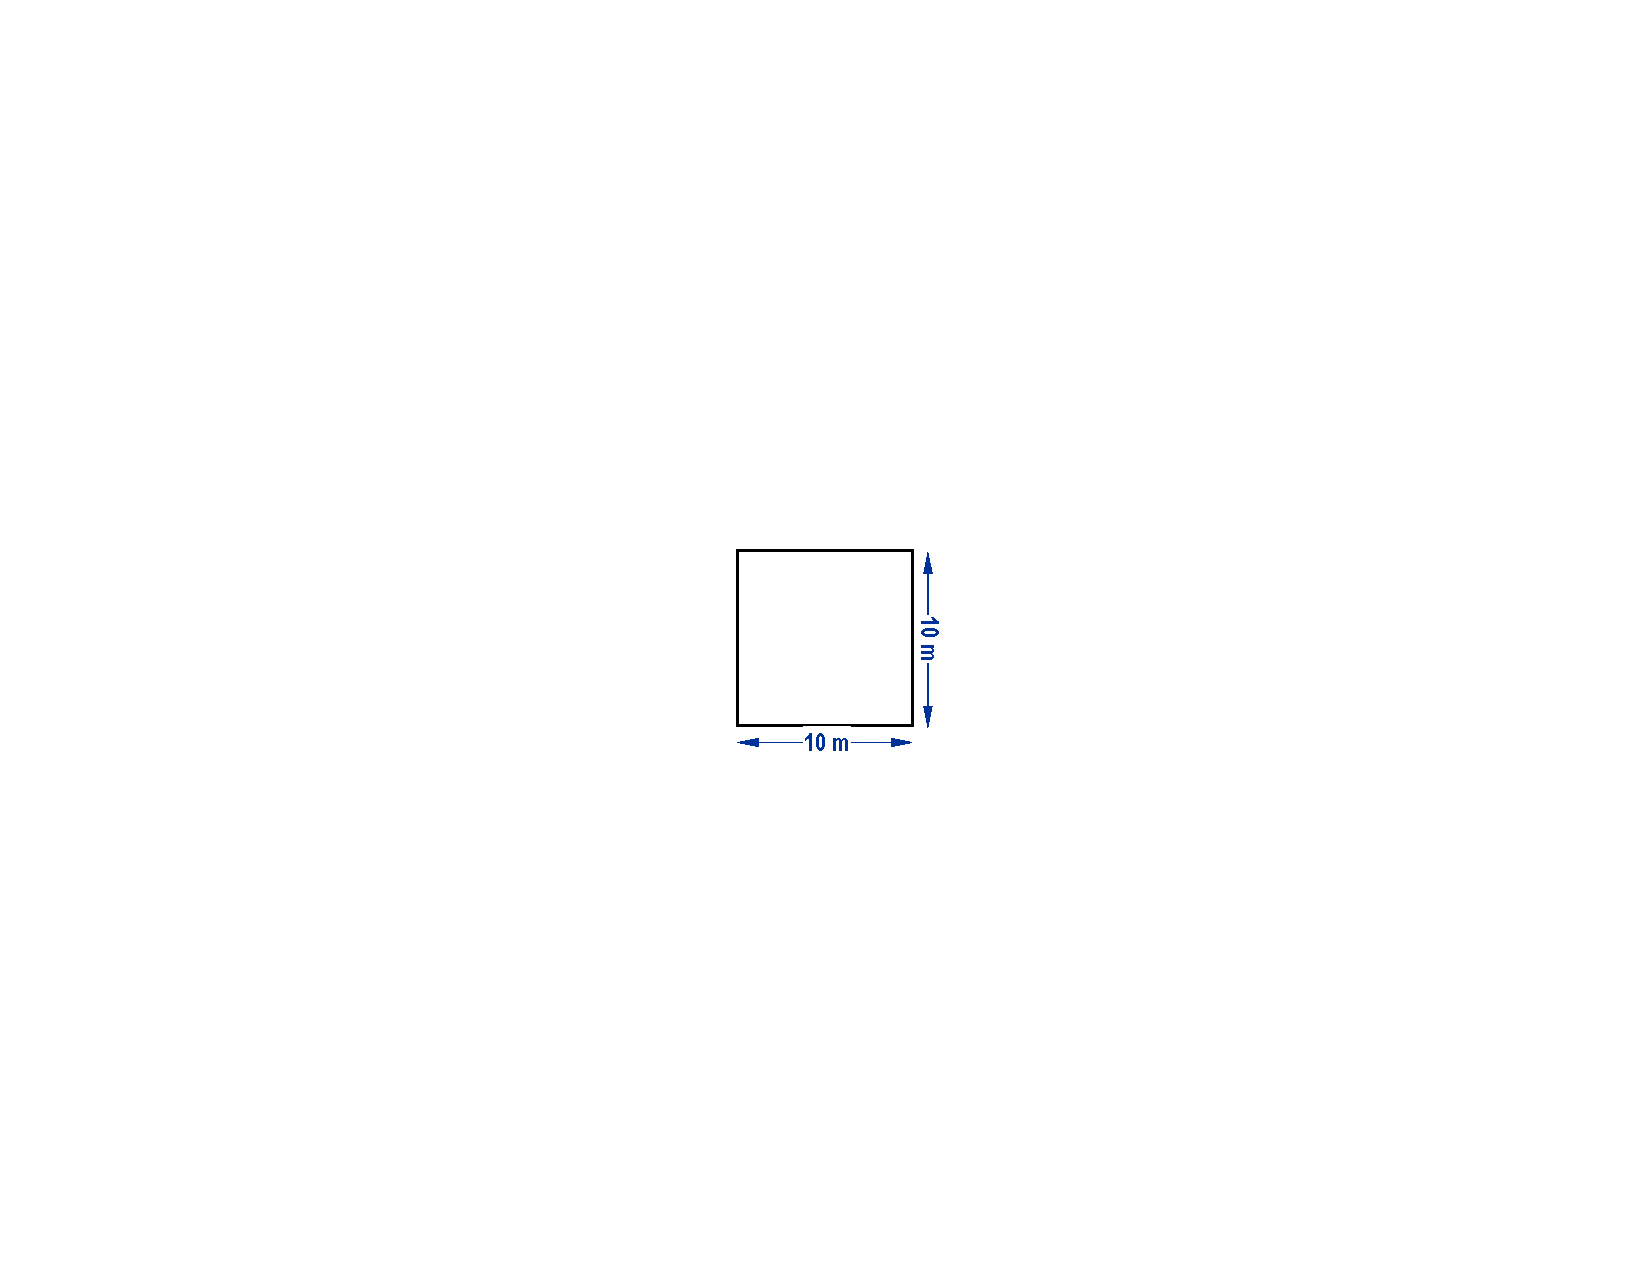
\includegraphics[width=0.6\linewidth]{chapter4/FIGS/fig-pattern-square.pdf}\\
{(a) Square}\\
\end{minipage}
\begin{minipage}{0.5\linewidth}
\centering
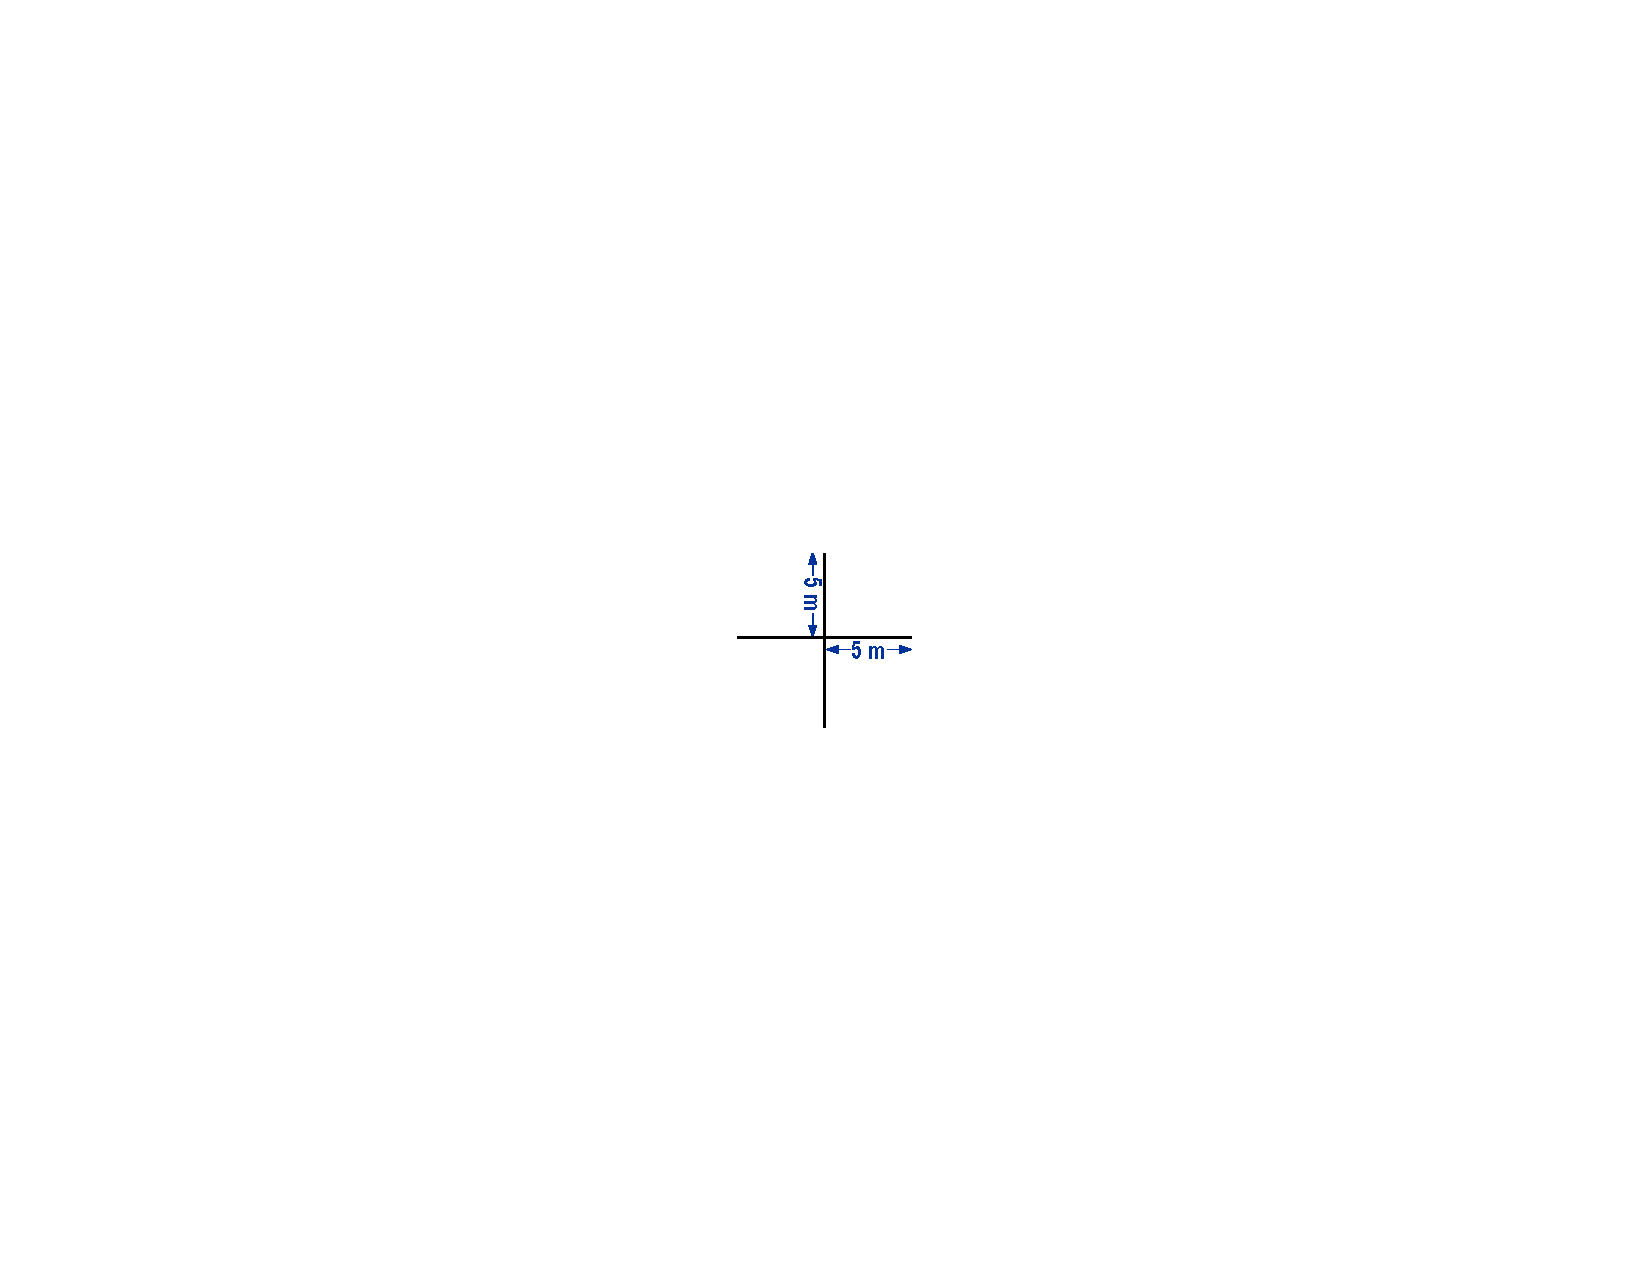
\includegraphics[width=0.6\linewidth]{chapter4/FIGS/fig-pattern-cross.pdf}\\
{(b) Cross}\\
\end{minipage}
\caption{Tracking Patterns}
\label{fig:patterns}
\end{figure}

\subsection{Task-3: Following at a Fixed Leash Distance}
\label{sec:task3}

\subsubsection{Task Description}
\label{sec:task3-desc}

Only limited actuation is needed to keep the target in the
drone's FOV in Task-2.  More substantial actuation is required for
Task-3.  After detecting a moving target, the drone moves to keep it
at a preset {\em leash distance.} This compounds latency issues as the
drone must now yaw and reposition itself correctly when the target
maneuvers quickly. At high target speeds (over 2.5~m/s), this can
prove difficult because even small actuation mistakes can result in
total loss of visual contact. Although the Anafi Ai can statically
track moving objects, it does not have a 
following feature which makes a direct comparison of its performance infeasible.

I programmed the target to move at a constant speed over flat ground
in a specified pattern.  I used speeds of 1.5~m/s (slow), 2.5~m/s
(medium), and 3.5~m/s (fast).  These speeds roughly correspond to a
person walking, jogging slowly, and running.  Two patterns were used:
a square of side 10~m~(Figure~\ref{fig:patterns}(a)), and a cross with
four arms of 5~m each~(Figure~\ref{fig:patterns}(b)).  The square
embodies abrupt change of trajectory after 10~m of straight line travel,
while the change of trajectory in the cross occurs after only 5~m. As in Task-1, the drone is initially hovering at fixed altitude.  I used altitudes of 5~m and 10~m in my experiments, but omitted 15~m
since Section~\ref{sec:task1-results} indicates poor performance at this altitude. 

\subsubsection{Algorithm}
\label{sec:tracking-algorithm-advanced}
The algorithm used for this experiment is a modified version of the one used in Section~\ref{sec:task2}. Once the target is detected, the drone tracks it by centering the bounding box in the frame. At the same time, it estimates its distance to the target, and moves such that it preserves a preset \textit{leash distance}. This leash distance is chosen before the experiment to adequately frame the target at the specified altitude. If the drone loses sight of the target, it hovers until
the object moves back into its FOV. No active search is made
by the drone to reacquire a lost target.

\subsubsection{Results}
\label{sec:task3-results}

I use the same scoring rubric of ``Success,'' ``Slow Actuation,'' and
``Fail'' as for Task-2.  At a target speed of 1.5~m/s, the results for
all runs in Table~\ref{tab:task3-results-5m-square} confirm
successful tracking with only occasional failure.  When speed
increases to 2.5~m/s, and then to 3.5~m/s, the number of failures
increases sharply.  This is consistent with the computer vision
processing pipeline following real-world scene changes too slowly, due
to the very low frame rate~(0.7~fps).  I show
later~(\S\ref{sec:discussion-results}) that increasing frame rate
improves tracking.  The effects of anomalously high LTE latency are
visible in Run 3.  This points to the challenge of using public
cellular networks which can experience unpredictable changes in bandwidth and latency.

\begin{table}
	\centering\small
	\begin{tabular}{|c|c|c|c|c|c|c|}
		\hline
		Speed & Run & Total & \multicolumn{2}{c|}{Success} & Slow & Fail\\
		(m/s) &  & Frames  & \multicolumn{2}{c|}{\footnotesize (Target Present)} & Act- &  \\
		\cline{5-5} 
		&  &         &         & $\rm \frac{Present}{Total}$ & uation  & \\ 
		\hline
		& 1 & 82 & 80 & & 1 & 1 \\
		1.5 & 2 & 85 & 76 & 95.2\% \scriptsize{(5\%)}  & 0 & 9 \\
		& 3 & 77 & 76 & & 1 & 0\\
		\hline
		& 1 & 82 & 49 & & 2 & 31 \\
		2.5 & 2 & 84 & 50 & 55\% \scriptsize{(8\%)} & 4 & 30 \\
		& \cellcolor{red!30}3 & \cellcolor{red!30}83 & \cellcolor{red!30}38 & & \cellcolor{red!30}0 & \cellcolor{red!30}45 \\
		\hline
		& 1 & 87 & 46 & & 2 & 39 \\
		3.5 & 2 & 84 & 60 & 62.7\% \scriptsize{(9.3\%)} & 1 & 23  \\
		& 3 & 83 & 53 & & 4 & 26 \\
		\hline
	\end{tabular}
	\begin{captext}
		\centering \\[0.1cm] Figures in parentheses are standard deviations.\\
		Abnormally high LTE latency was observed during the red highlighted run. This is always a possibility when using public cellular infrastructure. During high latency events, the performance of the system suffers considerably.
	\end{captext}
	\caption{Task-3 Results {\small (Altitude = 5~m, Pattern = Square)}}
	\label{tab:task3-results-5m-square}
\end{table}


Table~\ref{tab:task3-results-5m-cross} presents Task-3 results when
the pattern used is a cross rather than a square.  Comparing the
``Fail'' columns of Tables~~\ref{tab:task3-results-5m-square} and
\ref{tab:task3-results-5m-cross}, there is a noticeable decrease in
failures at speeds of 2.5~m/s and 3.5~m/s when the pattern is a cross.
These results are consistent with the cross being less demanding than
the square for tracking.

\begin{table}
\centering\small
\begin{tabular}{|c|c|c|c|c|c|c|}
\hline
Speed & Run & Total & \multicolumn{2}{c|}{Success} & Slow & Fail\\
(m/s) &  & Frames  & \multicolumn{2}{c|}{\footnotesize (Target Present)}& Act-  &  \\
\cline{5-5} 
      &  &         &         & $\rm \frac{Present}{Total}$ & uation  & \\ 
\hline
    & 1 & 83 & 83 &    & 0 & 0 \\
1.5 & 2 & 88 & 88 & 100\% \scriptsize{(0\%)} & 0 & 0 \\
    & 3 & 78 & 78 &    & 0 & 0 \\
\hline
    & 1 & 85 & 67 &        & 0 & 18 \\
2.5 & 2 & 80 & 75 & 88.6\% \scriptsize{(8.5\%)} & 0 &  5 \\
    & 3 & 88 & 82 &        & 1 &  5 \\
\hline
    & 1 & 82 & 82 &        & 0 &  0 \\
3.5 & 2 & 85 & 59 & 89\% \scriptsize{(17\%)} & 1 & 25 \\
    & 3 & 86 & 84 &        & 2 &  0 \\
\hline
\end{tabular}
\begin{captext}
\centering \\[0.1cm] Figures in parentheses are standard deviations. \\
\end{captext}
\caption{Task-3 Results {\small (Altitude = 5~m, Pattern = Cross)}}
\label{tab:task3-results-5m-cross}
\end{table}

\begin{table}
	\centering\small
	\begin{tabular}{|c|c|c|c|c|c|c|}
		\hline
		Speed & Run & Total & \multicolumn{2}{c|}{Success} & Slow & Fail\\
		(m/s) &  & Frames  & \multicolumn{2}{c|}{\footnotesize (Target Present)}& Act-  &  \\
		\cline{5-5} 
		&  &         &         & $\rm \frac{Present}{Total}$ & uation  & \\ 
		\hline
		& 1 & 83 & 65 & & 1 & 17 \\
		1.5 & 2 & 78 & 74 & 81.6\% \scriptsize{(12\%)}  & 0 & 4 \\
		& 3 & 88 & 63 & & 3 & 19\\
		\hline
		& 1 & 82 & 52 & & 2 & 39 \\
		2.5 & 2 & 83 & 48 & 62.3\% \scriptsize{(4\%)} & 1 & 34 \\
		& 3 & 87 & 57 & & 0 & 30 \\
		\hline
		& 1 & 88 & 57 & & 1 & 30 \\
		3.5 & 2 & 83 & 45 & 64.8\% \scriptsize{(10.5\%)} & 1 & 37  \\
		& 3 & 89 & 67 & & 3 & 19 \\
		\hline
	\end{tabular}
	\begin{captext}
		\centering \\[0.1cm] Figures in parentheses are standard deviations. \\
	\end{captext}
	\caption{Task-3 Results {\small (Altitude = 10~m, Pattern = Square)}}
	\label{tab:task3-results-10m-square}
\end{table}


At an altitude of 10~m, the drone's FOV is increased, but there is a
significant drop in precision and recall as shown in
Table~\ref{tab:task1-results}~(b).  This leads to an increase in the
number of tracking failures relative to 5~m, regardless of the target
pattern or speed.  The effect is most apparent at the slowest speed:
the results for 1.5~m/s in Table~\ref{tab:task3-results-10m-square}
show higher failures than the results at 1.5~m/s in
Table~\ref{tab:task3-results-5m-square}.  Similarly, the results for
1.5~m/s in Table~\ref{tab:task3-results-10m-cross} show higher
failures than the results for 1.5~m/s in
Table~\ref{tab:task3-results-5m-cross}. These effects persist at
higher speeds, but are less obvious.  The improvement at
2.5~m/s between Tables~\ref{tab:task3-results-5m-square} and
\ref{tab:task3-results-10m-square} is due to the high-latency LTE
anomaly mentioned earlier.

\begin{table}
	\centering\small
	\begin{tabular}{|c|c|c|c|c|c|c|}
		\hline
		Speed & Run & Total & \multicolumn{2}{c|}{Success} & Slow & Fail\\
		(m/s) &  & Frames  & \multicolumn{2}{c|}{\footnotesize (Target Present)}& Act-  &  \\
		\cline{5-5} 
		&  &         &         & $\rm \frac{Present}{Total}$ & uation  & \\ 
		\hline
		& 1 & 80 & 75 &    & 0 & 5 \\
		1.5 & 2 & 85 & 85 & 87.3\% \scriptsize{(16.8\%)} & 0 & 0 \\
		& 3 & 85 & 58 &    & 0 & 27 \\
		\hline
		& 1 & 84 & 67 &        & 0 & 17 \\
		2.5 & 2 & 81 & 81 & 86.6\% \scriptsize{(11.6\%)} & 0 &  0 \\
		& 3 & 85 & 68 &        & 0 &  17 \\
		\hline
		& 1 & 86 & 62 &        & 0 &  24 \\
		3.5 & 2 & 86 & 85 & 82.9\% \scriptsize{(14.1\%)} & 1 & 0 \\
		& 3 & 86 & 67 &        & 1 &  18 \\
		\hline
	\end{tabular}
	\begin{captext}
		\centering \\[0.1cm] Figures in parentheses are standard deviations. \\
	\end{captext}
	\caption{Task-3 Results {\small (Altitude = 10~m, Pattern = Cross)}}
	\label{tab:task3-results-10m-cross}
\end{table}

\subsection{Task-4: Close Inspection}
\label{sec:task4}

\subsubsection{Task Description}
\label{sec:task4-desc}

Task-4 corresponds to the classic active vision tactic of ``taking a
closer look'' that was mentioned earlier~(\S\ref{sec:introduction}).   It
begins with the drone hovering at 15~m.  As in Task-1, the target
moves in a freeform path that is manually controlled over WiFi.  When
the target is detected in the FOV of the drone, confirmation at the
lower altitude of 5~m is attempted.  During the descent, the target is
kept in the FOV using yaw and gimbal actuation; the drone's
pitch and roll are not modified.  If multiple targets are detected at
15~m, only confirmation of the highest-confidence detection is
attempted.



\subsubsection{Results}
\label{sec:task4-results}

The results for Task-4 are shown in Table~\ref{tab:task4-results}.
The row labeled ``Static 15~m'' correspond to the 15~m results from
Table~\ref{tab:task1-results}~(b).  Relative to that baseline, both
precision and recall improve by nearly 30\% by ``taking a closer
look.''  There is, of course, a cost in time because actuation
involves physical motion of the drone to the lower altitude.  Further,
the increased FOV at higher altitude offers wider coverage.  For these
reasons, better accuracy at higher altitude will always be valuable.
However, when such improvement is not possible due to limitations of
the drone's optical system or processing pipeline, autonomously
descending to a lower altitude for target confirmation can be
effective.

\begin{table}
	\centering\small
		\centering\small
			\begin{tabular}{|c|c|c|}
			\hline
			Altitude& Precision & Recall\\
			\hline
			Close Inspection (15m-5m) & 0.94 & 0.68 \\
			Static 15 m (\S\ref{sec:task1-results}) & 0.65 & 0.33 \\
			\hline
		\end{tabular}\\
		\caption{Task-4 Results}
		\label{tab:task4-results}
\end{table}

\subsection{Task-5: Obstacle Avoidance}
\label{sec:task5}

\subsubsection{Task Description}
\label{sec:task5-desc}

\begin{figure}
\vspace{0.1in}
\begin{minipage}[b]{0.495\linewidth}
\centering
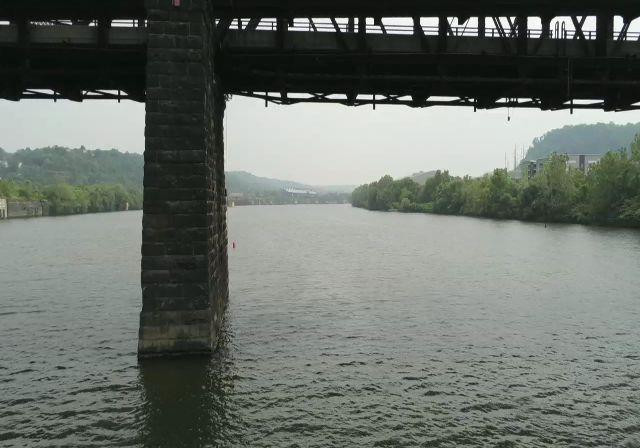
\includegraphics[width=0.95\linewidth]{chapter4/FIGS/fig-bridge-raw.jpg}\\
{\small (a) Raw Input}\\
\end{minipage}
\begin{minipage}[b]{0.495\linewidth}
\centering
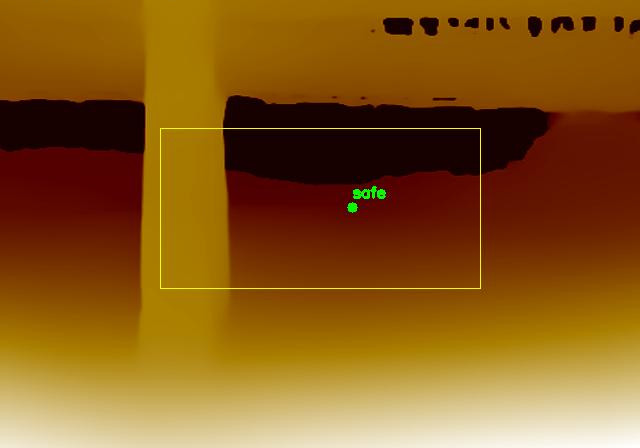
\includegraphics[width=0.95\linewidth]{chapter4/FIGS/fig-bridge-midas.jpg}\\
{\small (b) Output of MiDaS}\\
\end{minipage}
\caption{Bridge Obstacle Avoidance}
\label{fig:midas-sample}
\end{figure}

Task-5 compares my platform's monocular obstacle avoidance, using my
visual pipeline at 0.7~fps, with the stereoscopic obstacle avoidance
of the Anafi Ai using on-board computing at 30~fps.  I place the 2~m
tall by 0.5~m wide foam pillar used in Task-2~(\S\ref{sec:task2})
directly in the drone's path. The drone is instructed to fly at 1
m/s at a fixed altitude of 1~m directly towards the obstacle.  I
capture a trace of the drone's flight path across 3 different runs.

\begin{figure}
\begin{minipage}[b]{0.495\linewidth}
\centering
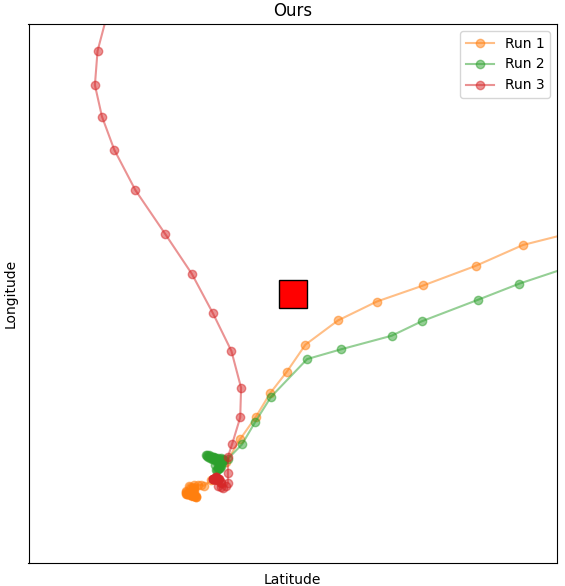
\includegraphics[width=0.95\linewidth]{chapter4/FIGS/fig-obstacle-path-ours.png}
{(a) SteelEagle}
\end{minipage}
\begin{minipage}[b]{0.495\linewidth}
\centering
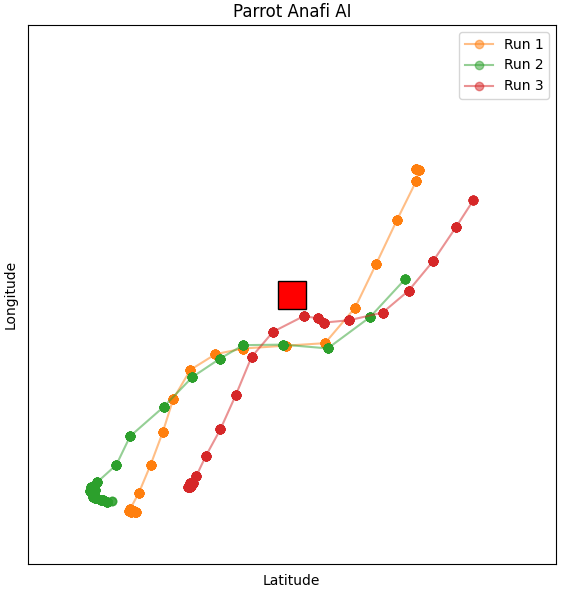
\includegraphics[width=0.95\linewidth]{chapter4/FIGS/fig-obstacle-path-anafiai.png}
{(b) Anafi Ai}
\end{minipage}
\caption{Task-5 Results}
\label{fig:obstacle-path}
\end{figure}

\subsubsection{Algorithm}
\label{sec:midas-algorithm}
Some drones utilize stereo cameras or LIDAR to detect and avoid
obstacles. These give accurate depth data (i.e., distance to objects),
allowing the drone to map out its environment and to calculate optimal
collision-free trajectories.  Since my drone is only equipped with a
monocular camera, it cannot infer depth via simple geometric methods.
I therefore use a DNN-based algorithm called MiDaS ~\cite{Ranftl2022}
to provide relative depth estimates.  Using MiDaS on each frame
received by the cloudlet, we construct the inverse relative depth map.
Based on the rate of change of relative depth across frames, we
identify obstacles in the flight path and actuate away from them.
Figure~\ref{fig:midas-sample}(a) shows an input frame from one of my
flights, as the drone approaches the obstacle course.
Figure~\ref{fig:midas-sample}(b) shows the depth-encoded output of my
algorithm on this frame.  The drone actuates towards the green dot
using a tuned PID-loop~\cite{Ang2005} to avoid the closest flags.
Once past these flags, it re-computes a new safe objective towards
which it can fly to avoid the second tier of flags.  It repeats these
steps until it is past all obstacles. This simple approach to obstacle
avoidance serves as a good experimental baseline.

\subsubsection{Results}
\label{sec:task5-results}

Figure~\ref{fig:obstacle-path}(a) plots the flight path of each run
for my platform, along with the position of the pillar.
Figure~\ref{fig:obstacle-path}(b) plots the flight paths of the Anafi
Ai on the same task.  Both platforms successfully avoid the obstacle
in all cases, but do so using very different tactics. The
low frame rate and high end-to-end latency of my pipeline forces my
platform to be very conservative, and to give the obstacle a wide
berth.  Well past the obstacle, the drone has not yet returned to its
original flight path.  In contrast, the stereoscopic cameras, high
frame rate and low end-to-end processing latency of the Anafi Ai
together enable it to be much less conservative in obstacle avoidance.
The flight paths cluster more tightly around the obstacle, and the drone
soon returns to its original flight path.

\section{Summary of Results}
\label{sec:take-away}

My evaluation began with a single top-level question.  Could
autonomous active vision be successfully implemented on a drone with
severe constraints on both local compute and offloading?  The maximum
offloading throughput of 0.7~fps imposed by LTE thermal constraints on
the watch~(\S\ref{sec:stream-in-practice}) is a severe bottleneck.  The
heavy-tailed distribution of end-to-end processing pipeline latency,
with a mean of over 1~s~(\S\ref{sec:event-to-detection-latency}), is another
bottleneck.  Combined with limitations of onboard processing on the
watch and the quality of the drone's optical system, these constraints
pose a formidable barrier.

In spite of this barrier, the results presented~(\S\ref{sec:task1} to
\S\ref{sec:task5}) show that active vision capabilities such as
tracking a moving object and confirming object detection by dropping
to lower altitude are feasible at credible target speeds.  Even with
the current implementation, one can perform useful tasks involving
active vision.  The range of feasible tasks can be broadened via
hardware advancements in the drone and the watch, combined with more
sophisticated algorithms that can then be supported.  Progress on this
front would also enable the superior resources of the cloudlet to be better
utilized.  Right now, the benefit of the cloudlet is being muted by the low
sustainable offloading rate. Even so, thanks to the modular design of SteelEagle, it is still possible to port new AI algorithms with minimum effort into the pipeline which could perform better on this limited stream.

\section{Benefit of Increased Frame Rate}
\label{sec:discussion-results}

The results for Task-3~(\S\ref{sec:task3}) make it clear that the
drone's frame rate of 0.7~fps is a major limiting factor for tracking.
When tracking high speed objects that perform erratic maneuvers, the
drone often only has one or two detections to actuate upon. It often
does not get feedback on actuation errors until the target has exited
the frame entirely. Once that happens, tracking fails and the target
is lost.

To quantify the benefits of a higher frame rate, I repeated the most
difficult combination of speed and pattern in my Task-3 experiments:
3.5~m/s for a square pattern. Instead of using the watch, I used a
ground-based laptop to play exactly the same role.  The laptop
connects to the drone over WiFi, and connects to the cloudlet via a
commercial cellular LTE network.  In every respect other than the fact
that the laptop is not flying with the drone, the processing
pipeline is unchanged from  Figure~\ref{fig:sys-arch}.
The tracking algorithm is also unchanged from that described for
Task-3~(\S~\ref{sec:task3}). Although the laptop experiences the same
WiFi, RTSP video stream, and LTE conditions as the watch did, it does
not suffer from the same processing or LTE thermal limitations.  This
enables offloading of video processing to the cloudlet a much higher frame
rate. I chose a figure of 3~fps since I believe that this is
realistically achievable with slightly better watch hardware. Even the
Samsung Galaxy 4 watch can sustain 3~fps for over two minutes if it is
pre-cooled with an ice pack.  This is the full length of one run of
Task-3~(\S~\ref{sec:task3}).

\begin{table}
        \centering\small
        \begin{tabular}{|c|c|c|c|c|c|c|}
                \hline
                Frame & Run & Total & \multicolumn{2}{c|}{Success} & Slow & Fail\\
                Rate  &  & Frames  & \multicolumn{2}{c|}{{\footnotesize (Target Present)}}& Act-  &  \\
                \cline{5-5}
                (fps) &  &         &         & $\rm \frac{Present}{Total}$  & uation  & \\
                \hline
                & 1 & 361 & 283 &        & 1 &  77 \\
                3& 2 & 360 & 342 & 83.7\% \scriptsize{(9.8\%)} & 1 & 17 \\
                & 3 & 361 & 280 &        & 0 &  82 \\
                \hline
                    & 1 & 87 & 46 & & 2 & 39 \\
                0.7 & 2 & 84 & 60 & 62.7\% \scriptsize{(9.3\%)} & 1 & 23  \\
                & 3 & 83 & 53 & & 4 & 26 \\
                \hline
        \end{tabular}
        \begin{captext}
                \centering \\[0.1cm] Speed was 3.5~m/s.  Figures in parentheses are standard deviations.
        \end{captext}
        \caption{Increased Frame Rate {\footnotesize (Altitude = 5~m, Pattern = Square)}}
        \label{tab:taskfps-results}
\end{table}

\begin{table}
        \centering\small
        \begin{tabular}{|c|c|c|}
                \hline
                Platform & Weight (g) & Throughput (fps)\\
                \hline
                Galaxy Watch 4 & 26 & 1 \\
                Future Offload Device & $<$50 & 3\\
                Pixel 4a & 143 & 5 \\
                Dell Latitude 5420 Laptop & 2500+ & 6 \\
                \hline
        \end{tabular}\\
        \caption{Throughput and Weight by Platform}
        \label{tab:throughput}
\end{table}

\begin{table}
        \centering
        \begin{tabular}{|c|c|c|c|}
                \hline
                & Inference & Effective Throughput \\
                & (ms) & (fps) \\
                \hline
                Object & 56.3 & 17.8  \\
                Detection & (5.9) &  \\
                \hline
                Obstacle & 124.3 & 8.1 \\
                Avoidance & (4.9) &  \\
                \hline
        \end{tabular}
        \begin{captext}
                \centering \\[0.1cm] Standard deviation in parentheses. \\
        \end{captext}
        \caption{Cloudlet Performance}
        \label{tab:cloudlet-perf}
\end{table}

Table~\ref{tab:taskfps-results} presents my results for an altitude of
5~m.  For easy comparison, the 3.5~m/s results from
Table~\ref{tab:task3-results-5m-square} are reproduced below the new
results.  Increasing the frame rate from 0.7~fps to 3~fps greatly
improves tracking --- almost a 20\% increase in the ``Success''
column.  Even the worst run at 3~fps achieves 77.5\% success which is
6.1\% better than the best run at 0.7~fps at 71.4\%
success.  This improvement is obtained without modifying my tracking
algorithm. 

Since frame rate is such an important factor in successful tracking,
it is natural to speculate on what might be possible with future
hardware advancements.  For example, if a future offload device was no heavier
than it is today but had the processing power of today's smartphones,
how much better could it do tracking?  To gain some insight into these
speculative questions, I tested the processing pipeline of
Figure~\ref{fig:sys-arch} using different offload platforms.  Experiments were performed with an identical setup as in Section~\ref{sec:event-to-detection-latency}.

Table~\ref{tab:throughput} shows the throughput in fps and the weight
of various computing platforms today. The first two rows are the
current platform and a theoretical future offload device.  The third row is a Pixel 4a smartphone, which is able to sustain 5~fps. At 143~g, it is too heavy
for my drone to carry, but its 5x improvement in throughput is very
attractive for robust tracking. The fourth row is a Dell Latitude 5420
laptop, which is able to sustain 6 fps; clearly, its 2.5~kg weight is
far beyond the payload lift of any ultra-light drone.  Since the
laptop can decode video and transmit it over WiFi at 30~fps, the
bottleneck shifts to the LTE link and the cloudlet's DNN inference
time.  As Table~\ref{tab:cloudlet-perf} shows, the cloudlet is able
to inference at roughly 17.8~fps for object detection~(Task-1 to
Task-4) and 8.1~fps on obstacle avoidance~(Task-5). Thus, an improved offload device on the drone could take better advantage of cloudlet resources. In the next chapter, I explore possible replacement devices for the watch in order to quantify this improvement.





\chapter{A New Offload Device}
The watch prototype is severely limited in its ability to deliver a high throughput and low latency video stream to the edge, hindering the benefits of edge computing. In order to better take advantage of cloudlet resources, a new offload device is needed which can transmit the video stream without the thermal restrictions of the watch. As discussed in Section~\ref{sec:achieving-cell-conn}, there are no current Android products other than smart watches that satisfy the stringent weight requirements of the Parrot Anafi platform. The only path forward is to explore other segments of the mobile computing landscape.

In this chapter, I propose a new offload device which fixes some of the shortcomings of the watch prototype. I will show how it improves upon the watch in some ways but fails to match its capabilities in others. In Section~\ref{sec:watch-replacement}, I explain the process of choosing a new device. I give a breakdown of its control model and how it differs from the watch. In Section~\ref{sec:e2e-latency}, I use an agility analysis framework to compare the overall performance of each prototype.

\section{Finding a Watch Replacement}
\label{sec:watch-replacement}

For any device to replace the watch, it must satisfy three main requirements of the SteelEagle pipeline: WiFi connectivity, cellular connectivity, and light weight. The first two requirements, WiFi and cellular connectivity, are relatively easy to find within the mobile device space. Meeting the weight requirement is much harder. The Parrot Anafi was able to fly with the watch payload, around 39~g, but was unable to fly with the Unihertz Jelly Pro payload, around 90~g with EMI shielding included. This gives an approximate weight range for a watch replacement.

\subsection{Single-Board Computers}

Outside of smart watches, the only devices that lie within this weight range are single-board computers (SBCs). SBCs are small form factor computers which live on a board about the size of a credit card. They are widely used for internet of things (IoT) projects because of their small size, low power draw, and connectivity (usually WiFi but sometimes cellular as well). The most popular SBC at the time of writing this dissertation is the Raspberry Pi~\cite{RaspberryPi}. The Pi is an Ubuntu SBC available in several sizes, the lightest of which is the Pi Zero 2 W at 16~g (Figure~\ref{fig:pi-zero}). The Zero is equipped with a quad-core 1~GHz CPU and 512~MB of RAM. It has built-in WiFi connectivity but must be augmented with a dongle for cellular connectivity. Additionally, it does not come with an integrated battery, so it must be powered by an external power pack that provides 1.2~A at 5.5~V. I determined that EMI shielding was not needed since the Pi did not create enough interference to hinder the Anafi's compass. With a power pack, 4G LTE dongle, and mount included, a Pi Zero payload for the Anafi would reach around 80~g. From experimentation, I found this was too heavy as the drone exhibited poor flight characteristics. A lighter alternative was needed.

\begin{figure}
    \centering
    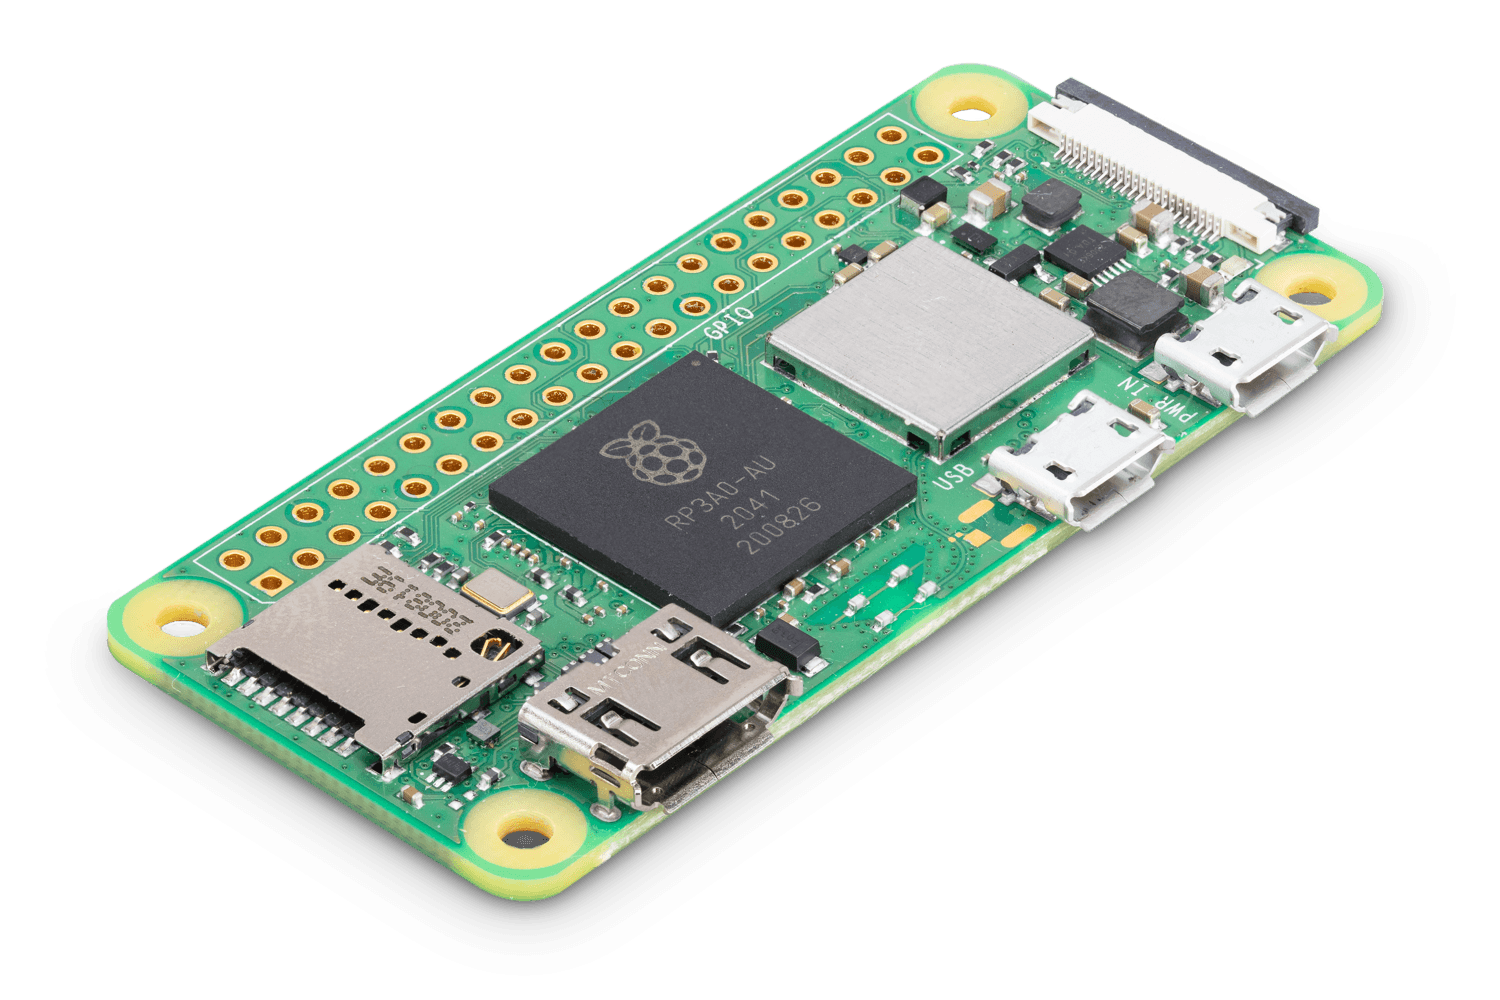
\includegraphics[width=0.4\linewidth]{chapter5/FIGS/zero2.png}
    \begin{captext}
    \small \\[0.1cm] The Pi Zero 2 W is 16~g but lacks cellular connectivity and requires an external power source. 
    \end{captext}
    \caption{Raspberry Pi Zero 2 W~\cite{RaspberryPi}}
    \label{fig:pi-zero}
\end{figure}

\begin{figure}
    \centering
    \vspace{-0.5in}
    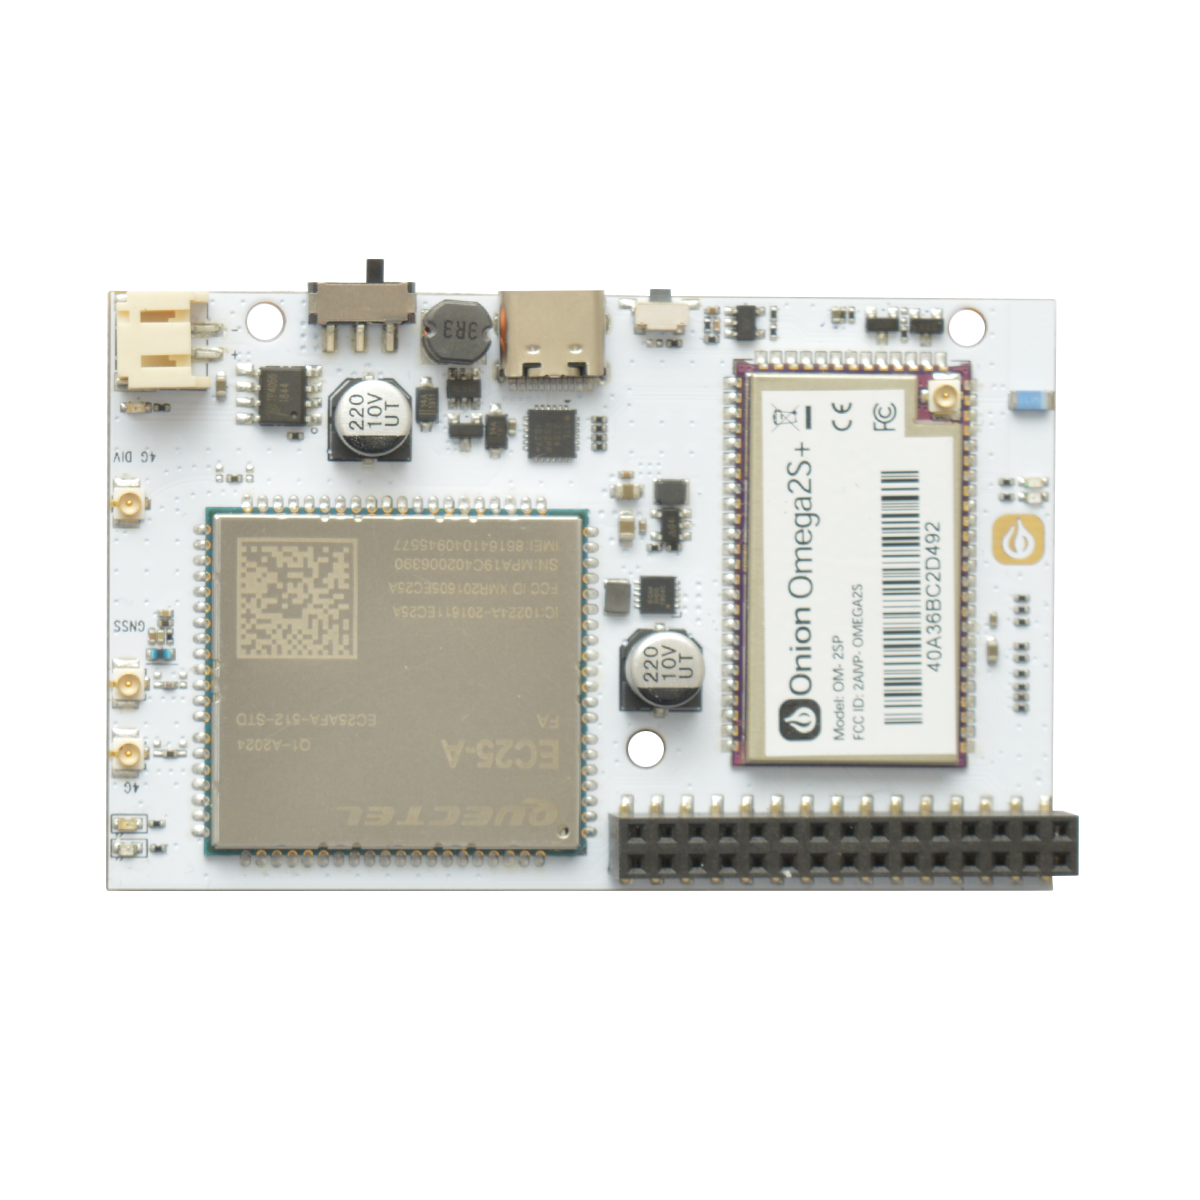
\includegraphics[width=0.4\linewidth]{chapter5/FIGS/onion.png}
    \vspace{-0.5in}
    \begin{captext}
    \small \\[0.1cm] The Onion Omega is 20~g with embedded WiFi and 4G. It requires a 3.3~V, 0.5~A power source. 
    \end{captext}
    \caption{Onion Omega 2 LTE~\cite{Onion}}
    \label{fig:onion}
\end{figure}

After an extensive search, I settled on the 20~g Onion Omega 2 LTE (Figure~\ref{fig:onion})~\cite{Onion}. The Omega is another SBC with built-in WiFi and 4G LTE connectivity. It runs OpenWRT Linux and is equipped with a single-core 580~MHz CPU and 128~MB of RAM. This makes it much less powerful, on paper, than the Galaxy Watch 4 (1.18~GHz dual-core CPU, 1.5~GB RAM). It also does not have an integrated battery, and like the Pi, does not create enough interference to warrant EMI shielding. However, unlike the Pi, the Onion only requires 0.5~A at 3.3~V which allows it to be powered by a much smaller, lighter power pack. This means, after adding a mount, power pack, and antennas, the Onion payload is a much slimmer 53~g. Through experimentation, I found this weight to be viable for sustained flight without adverse flight effects.

\begin{figure}
    \centering
    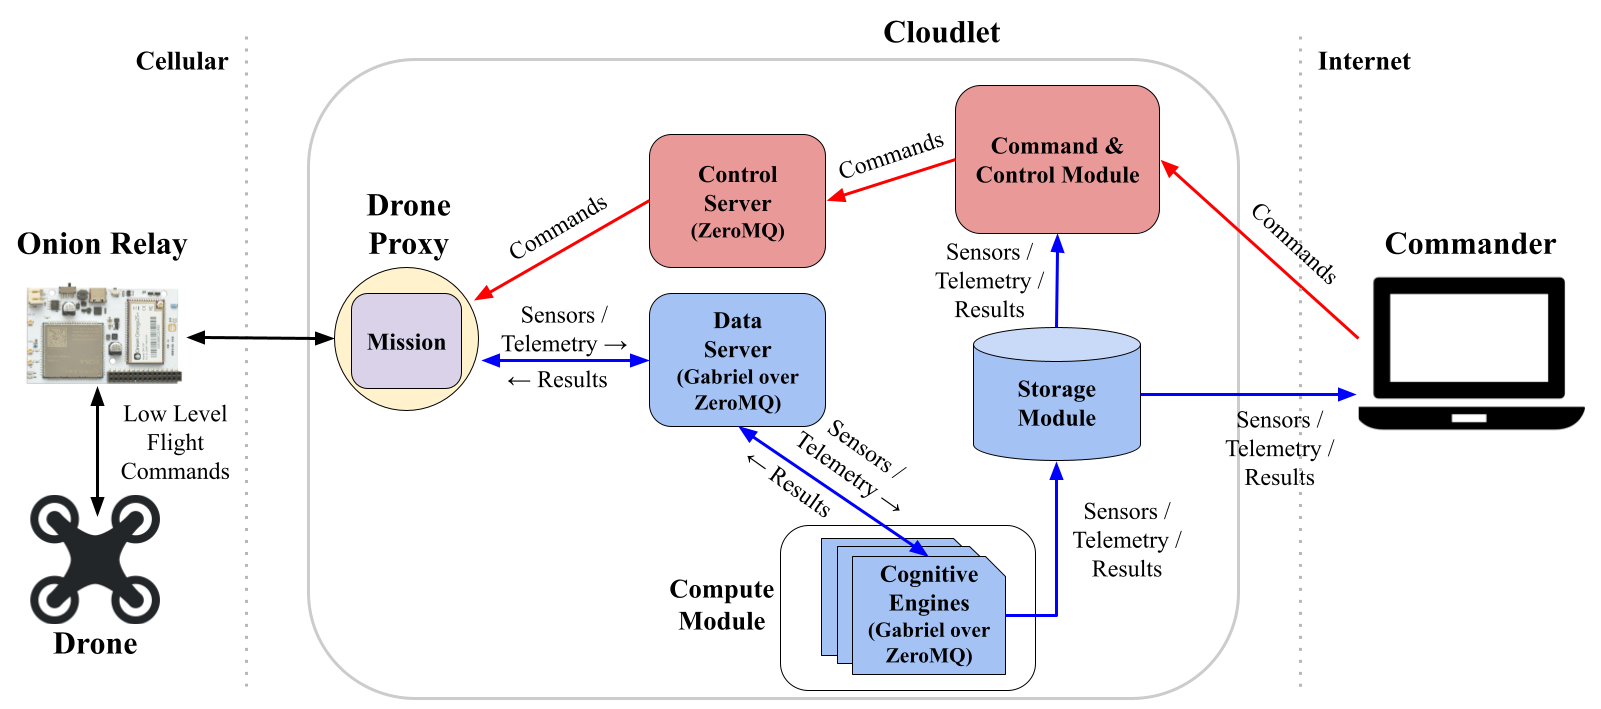
\includegraphics[width=1.0\linewidth]{chapter5/FIGS/arch-onion.png}
    \begin{captext}
    \\[0.1cm]
        \small The Onion acts as a pure relay, ferrying low-level command packets from the drone to the cloudlet. There, they are collected by a ``drone proxy'' which acts similarly to the watch in Figure~\ref{fig:sys-arch}.
    \end{captext}
    \caption{SteelEagle System Architecture with Onion Omega}
    \label{fig:sys-arch-onion}
\end{figure}

\subsection{The Onion Omega Payload}

The Onion's onboard compute resources are much worse than the Galaxy Watch 4. Its advantage is its thermals; it can run much, much hotter than the watch before overheating. This is mainly because it is not designed to be worn, and thus does not need to worry about burning its wearer. As a result, the Onion can transmit over its 4G link at a high rate without restrictions.

The Onion cannot run a full-featured local application like the watch can, but its ability to use cellular without constraints suggests a different control paradigm. Rather than controlling the drone locally from the watch and only sending frames to the cloudlet to run computer vision algorithms, the Onion can act as a pure relay, ferrying telemetry and video packets upstream while delivering command packets downstream. In this approach, the watch application would migrate to the cloudlet and would communicate with the drone over the Onion (Figure~\ref{fig:sys-arch-onion}).

This paradigm has some advantages. First, it theoretically allows the cloudlet to receive the raw video stream from the drone at full frame rate and relatively low latency (compared to the watch). Since the Onion does no video decoding, the latency cost paid is simply the transmission delay from the drone to the Onion over WiFi and from the Onion to the cloudlet over 4G. Second, the mission application lives on the cloudlet and so it can get computer vision results with negligible latency.

On the other hand, this setup has significant drawbacks compared to the watch. The Onion payload is not as accessible as the watch payload. It has exposed electronics and requires the use of a flammable LiPo power pack to use, whereas the watch is a consumer device that is easy to charge and is fully weatherproofed. Furthermore, since the Onion acts as a pure relay, it is at the mercy of its cellular connection. It cannot function separately from the cloudlet, while the watch can still pilot the drone without computer vision assistance. It also cannot adapt the video stream to reduced bandwidth by throttling, and must transmit the whole stream to produce usable frames on the backend.

Despite these problems, the Onion presents an opportunity to establish an upper bound for SteelEagle's performance. Where are the current bottlenecks in the system, and how can they be fixed? What is the best latency and throughput the system can achieve? How \textit{agile} is the system at reacting to new stimuli?

\subsection{A Framework for Understanding Agility: the \ooda~Loop}
To answer these questions, I introduce the concept of a drone \ooda~loop. Originally conceived in the 1950s to characterize
man-machine symbiosis in combat aircraft, this concept has
since been extended to many other domains~\cite{Boyd1986, Blaha2018, Johnson2023}.  The components of an \ooda~loop~(``Observe'', ``Orient,'' ``Decide,'' and
``Act'') define the stages of any reactive pipeline that involves a
human in the loop.  I extend this concept from its
cyber-human origins to the cyber-physical context of an autonomous
drone.  Viewing an AI pipeline through the lens of an \ooda~loop better explains its performance attributes.  It can tease apart latency and throughput limitations at fine granularity, thus enabling bottlenecks to be identified and optimized.

An \ooda~loop's attributes directly limit drone agility.  As discussed in Section~\ref{sec:event-to-detection-latency}, throughput limitations may cause closely-spaced real-world events to not be
resolvable as separate events.  High end-to-end latency
may cause slow reactions and punish mis-predictions. SteelEagle's \ooda~loop includes: (a) on-drone sensing, (b) on-drone
pre-processing, (c) transmission to cloudlet, (d) processing on a
(possibly multi-tenant) cloudlet, (e) transmission to drone, (f)
on-drone post-processing, and (g) drone actuation. I will profile and optimize these components through experimentation.

\begin{figure}
	\centering
	\includegraphics[width=0.85\linewidth]{FIGS/fig-simplified-arch.png}
	\caption{\small Edge Offload Pipeline}
	\label{fig:e2epipeline}
\end{figure}

\begin{figure}
	\definecolor{observe-color}{RGB}{175,208,149}
	\definecolor{orient-color}{RGB}{255, 255, 166}
	\definecolor{decide-color}{RGB}{255,170,149}
	\definecolor{act-color}{RGB}{224,194,205}
	\centering
	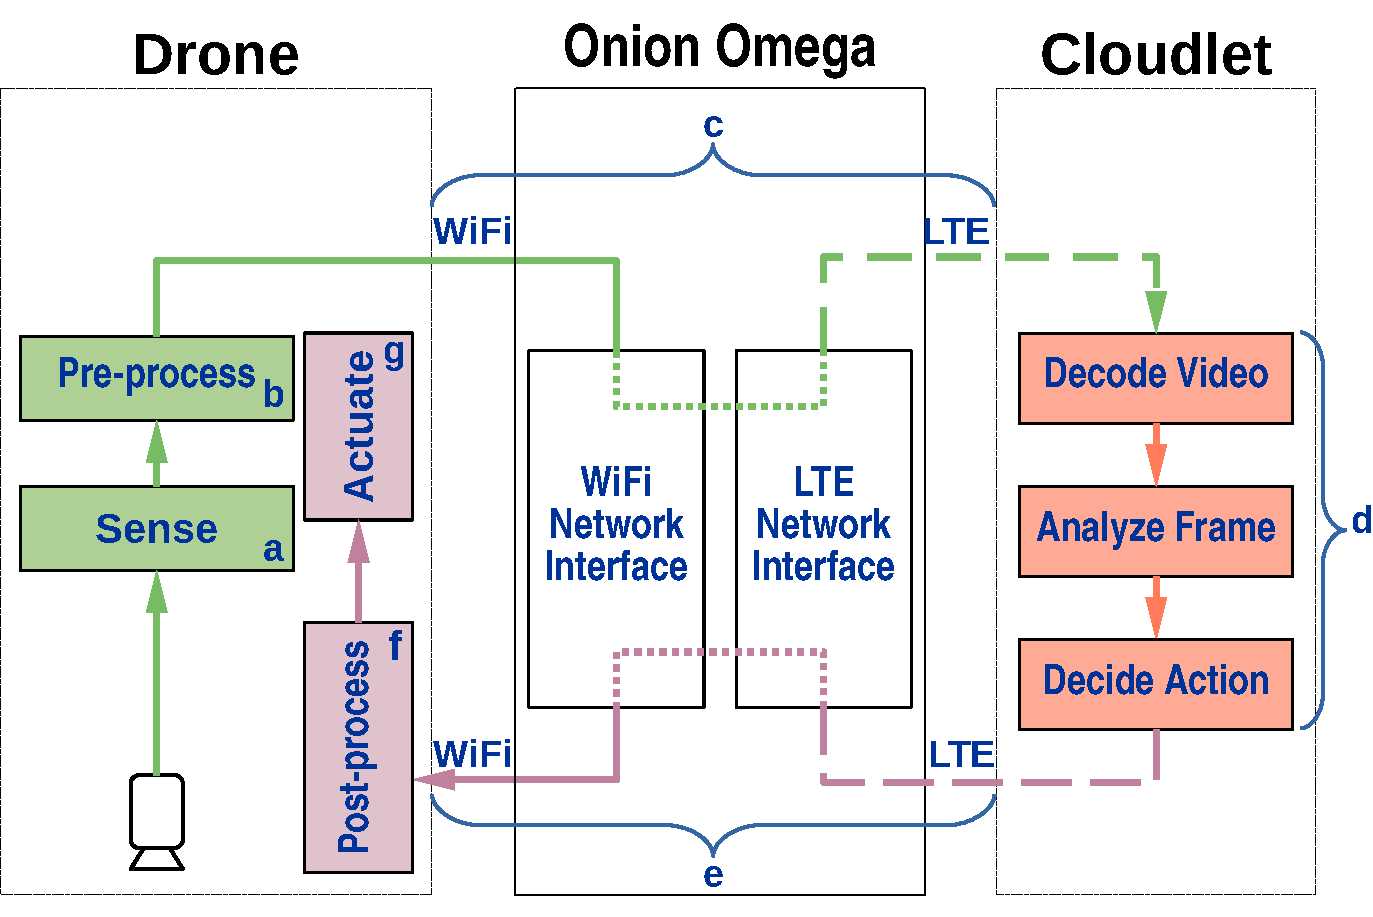
\includegraphics[width=0.9\linewidth]{FIGS/fig-ooda-loop.pdf}
	\begin{tikzpicture}
	    \draw[fill=observe-color] (1.0,0) rectangle (1.3,0.3);
	    \node[right] at (1.3,0.15) {\small Observe};
	
	    \draw[fill=decide-color] (2.9,0) rectangle (3.2,0.3);
	    \node[right] at (3.2,0.15) {\small Orient \& Decide};
	
	    \draw[fill=act-color] (5.7,0) rectangle (6.0,0.3);
	    \node[right] at (6.0,0.15) {\small Act};
	\end{tikzpicture}
	\caption{\small Detailed View of Our OODA Loop}
	\label{fig:ooda-loop}
	\vspace{0.2in}
	\centering
	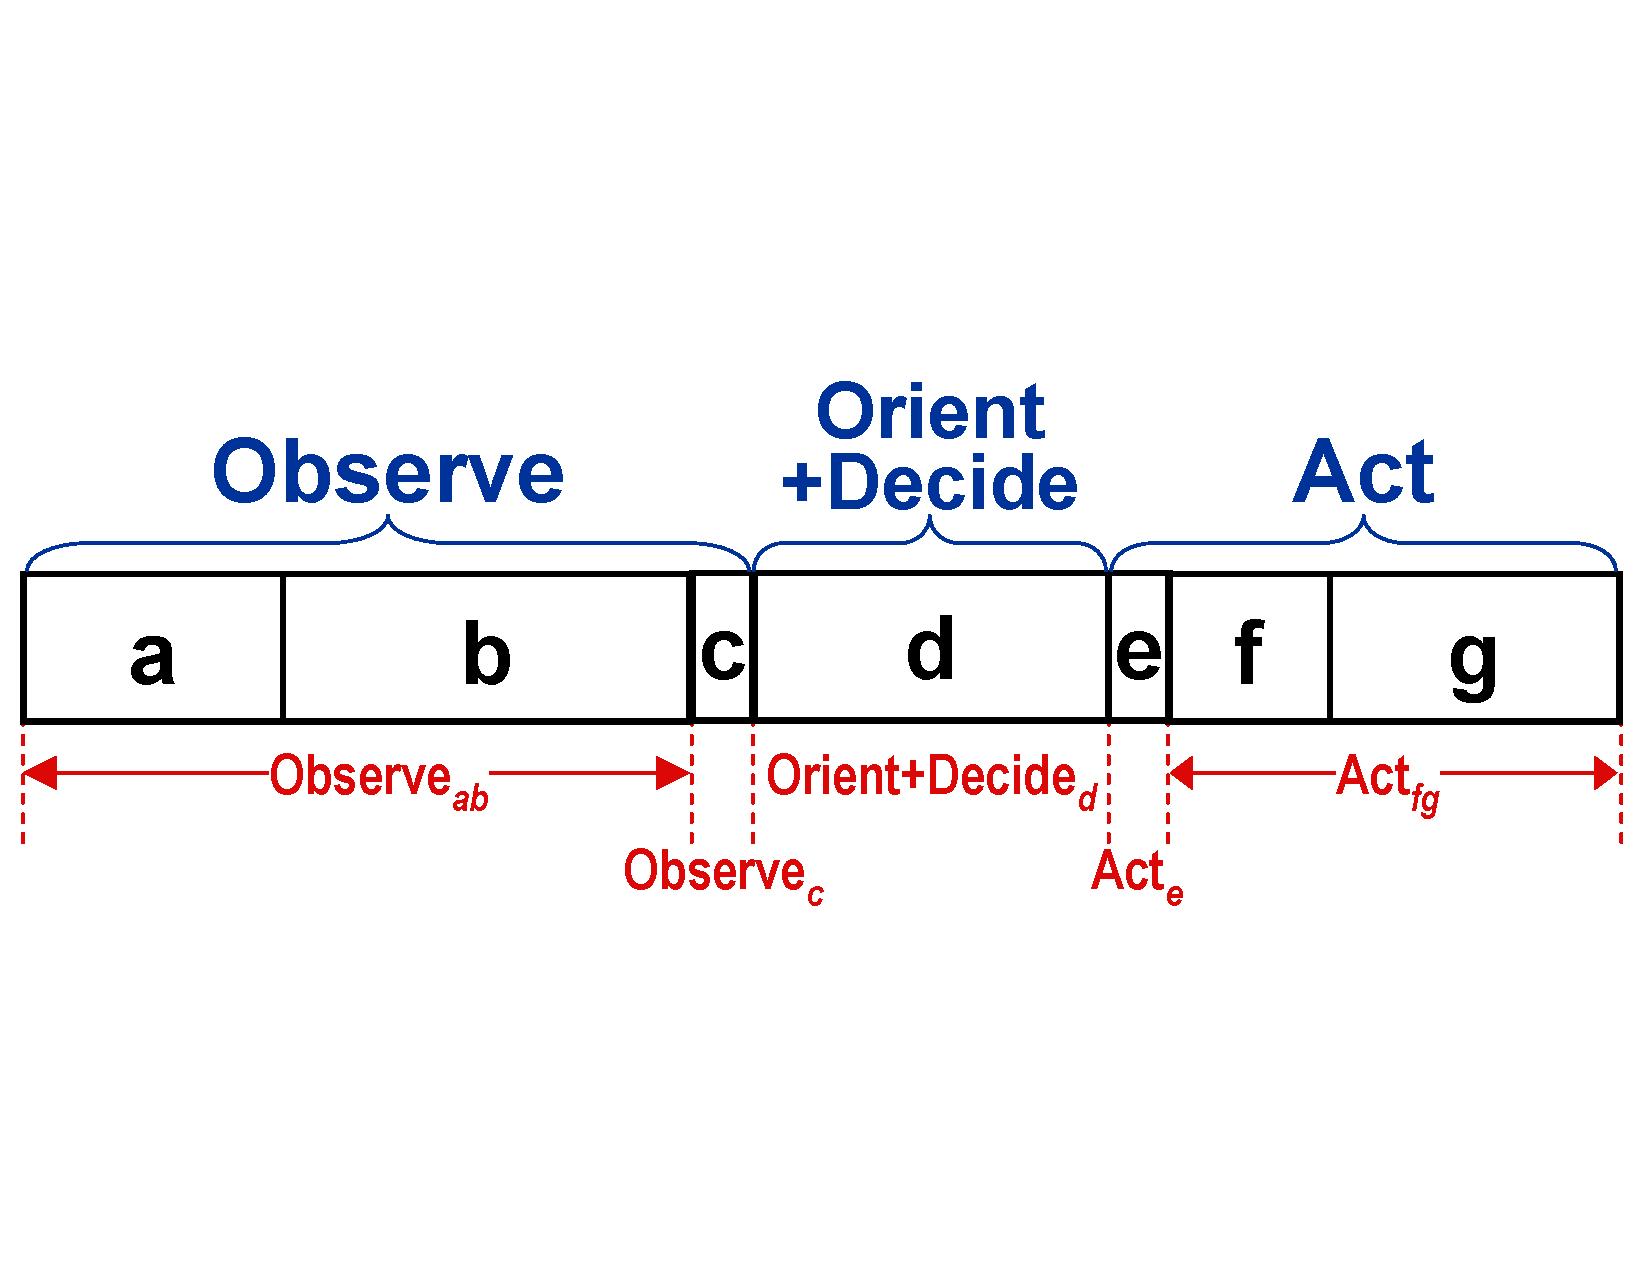
\includegraphics[width=0.9\linewidth]{FIGS/fig-ooda-nomenclature.pdf}
	\begin{captext}
		\centering Only items in \textcolor{red}{red} above can be measured.
		\flushleft
		\begin{tabular}{lll}
			\phantom{00} & a = on-drone sensing & e = transmission to drone\\
			\phantom{00} & b = on-drone pre-processing & f = on-drone post-processing\\
			\phantom{00} & c = transmission to cloudlet & g = drone actuation\\
			\phantom{00} & d = processing on cloudlet\\
		\end{tabular}
	\end{captext}
	\vspace{-0.1in}
	\caption{\small Measurable Components of Our OODA Loop}
	\label{fig:nomenclature}

\end{figure}

\section{Profiling \& Optimizing the \ooda~  Loop}
\label{sec:e2e-latency}

We replicate the setup~(Figure~\ref{fig:e2epipeline}) described by
Bala et al~\cite{Bala2023} using a slightly larger and heavier
variant~(550~g vs. 360~g) of the Parrot ANAFI drone. This variant is
approved on the BlueUAS list~\cite{BlueUAS2024} for US government
applications. As payload, we use the 53~g Onion Omega 2
LTE~\cite{Omega2023} single board computer which was briefly described
in that paper. The Onion Omega receives the sensor stream from the
drone over WiFi and forwards it to the cloudlet over 4G LTE.  The resulting
computation for Orient and Decide (e.g. DNN model
inference) causes a control message to be sent back via 4G LTE
to the Onion Omega, and thence over WiFi to the drone.

The drone to cloudlet pipeline is used for both data plane
and control plane operations.  Its intrinsic end-to-end performance
defines the experimental baseline.  To explore pipeline degradation,
we add network latency using FireQoS ~\cite{FireQoS} and drop frames
to throttle bandwidth.

\subsection{Mapping the OODA Loop}
\label{sec:mapping}

Figure~\ref{fig:ooda-loop} maps our end-to-end pipeline to \ooda~loop
components.  Components (a), (b) and (c) together map to the
``Observe'' phase; component (d) maps to its ``Orient'' and
``Decide'' phases; and, components (e), (f) and (g) together map to
the ``Act'' phase.  Due to closed-source restrictions of our COTS
pipeline, some \ooda~loop components have to be aggregated for
purposes of measurement, as shown by Figure~\ref{fig:nomenclature}.
Total end-to-end latency is given by the sum of these components;
total throughput is that of its bottleneck.

The earliest point in the pipeline where software instrumentation can
be inserted is between the Wi-Fi and LTE interfaces on the Onion
Omega.  The Wi-Fi part of this pipeline is thus attributed to
Observe$_{ab}$ rather than to Observe$_{c}$.  Similarly, on the return
path, the Wi-Fi part is attributed to Act$_{fg}$ rather than to
Act$_{e}$. Only LTE transmission is attributed to Observe$_{c}$ and
Act$_{e}$.  The resulting error is likely to be very small since Wi-Fi
is much more performant than LTE.  We present our detailed
measurements in \S\ref{sec:d2c-drone} to \S\ref{sec:c2d-drone}.


\subsection{Observe$_{ab}$}
\label{sec:d2c-drone}

Our drone is a commercial product that uses black box hardware and
software to seamlessly integrate (a) and (b).  Its camera creates a
stream of raw video frames.  On-board processing transforms these raw
frames into a sequence of UDP packets that slice-encode a 720p H.264
RTSP video stream at 30~fps~\cite{Schulzrinne2016}.  Neither the
resolution nor frame rate of this video stream are configurable.  The
slice encoding aims to reduce the visual impact of UDP packet loss.
The black box nature of this transformation makes attribution of
latency costs difficult.  It is not possible to insert instrumentation
to separate (a) and (b); they merge into an indivisible component.

\begin{figure}
\centering

\begin{minipage}[b]{.49\linewidth}
\centering
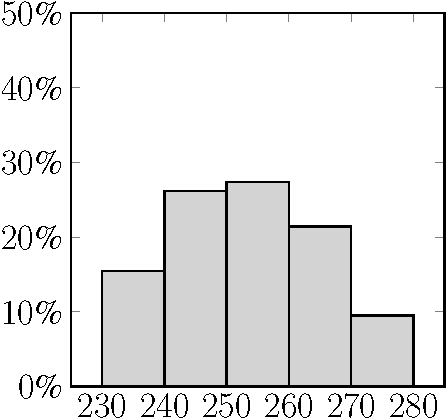
\includegraphics[width=0.97\linewidth]{histo-observeab-latency.pdf}
\begin{captext}
\centering
Mean: 253 $\pm 12$~ms\; p99: 277~ms\\
\end{captext}
\vspace{-0.05in}
{\small (a) Latency (ms)}
\end{minipage}
\begin{minipage}[b]{.49\linewidth}
\centering
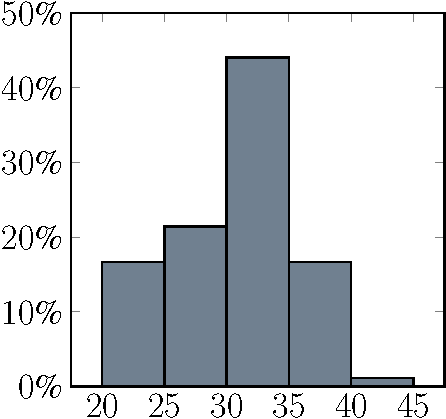
\includegraphics[width=0.97\linewidth]{histo-observeab-throughput.pdf}
\begin{captext}
\centering
Mean: 31~$\pm$5~fps\; p1: 22~fps\\
\end{captext}
\vspace{-0.05in}
{\small (b) Instant. Throughput (fps)}
\end{minipage}
\caption{\small Observe$_{ab}$ Measurements}
\label{fig:d2c-drone-histo}
\vspace{-0.1in}
\end{figure}

Figure~\ref{fig:d2c-drone-histo} presents our measurements.  The
latency distribution has a mean of 253~ms, with a standard deviation
of 12~ms and a p99 of 277~ms.  Instantaneous throughput has a mean of
31~fps, with a standard deviation of 5~fps and a p1 of 22~fps.  Due to
streaming, throughput can be higher than the reciprocal of latency.
The short WiFi Observe$_{ab}$ segment is partly responsible for this observed variation.

\subsection{Observe$_c$}
\label{sec:netdownlink}

As Figure~\ref{fig:e2epipeline} illustrates, the wireless network path
from drone to cloudlet consists of a very short Wi-Fi segment, transit
through the Onion router carried as payload, and then a longer 4G~LTE
segment to the cloudlet.  Figure~\ref{fig:d2c-net} presents the
latency and throughput distributions of Observe$_c$.  Its latency has
a mean of 39~ms, with a standard deviation of 8~ms and a p99 of 60~ms.
Instantaneous throughput has a mean of 16.3~Mbps, with a standard
deviation of 1~Mbps and a p1 of 14.4~Mbps.  Since 720p video at 30~fps
only demands an average bit rate of about 6.5~Mbps~\cite{Adobe2024},
Observe$_c$ is definitely not the bottleneck.


\begin{figure}
\vspace{0.1in}
\centering
\begin{minipage}[b]{.49\linewidth}
\centering
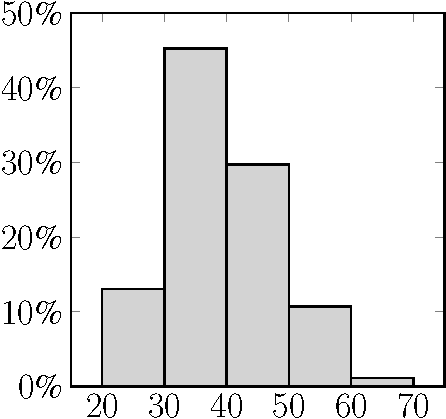
\includegraphics[width=0.97\linewidth]{histo-observec-latency.pdf}\\
\begin{captext}
\centering
Mean: 39~$\pm$8~ms\;p99: 60~ms\\
\end{captext}
\vspace{-0.05in}
{\small (a) Latency (ms)}
\end{minipage}
\begin{minipage}[b]{0.49\linewidth}
\centering
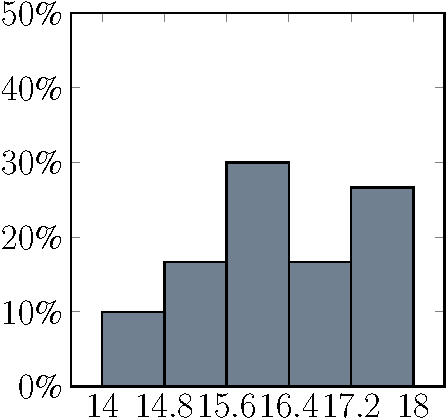
\includegraphics[width=0.97\linewidth]{histo-observec-throughput.pdf}\\
\begin{captext}
\centering
Mean: 16.3$\pm$1~Mbps p1: 14.4Mbps
\end{captext}
{\small (b) Throughput (Mbps)}
\end{minipage}
\vspace{-0.1in}
\caption{\small Observe$_c$ Measurements}
\label{fig:d2c-net}
\end{figure}

\subsection{Orient+Decide$_d$}
\label{sec:cloudlet}

Processing on the cloudlet involves three stages:
\begin{smitemize}

\item{Stage-1: Decoding the UDP packet stream to produce individual
    frames from H.264 video.}

\item{Stage-2: Application-specific processing of each frame to
    interpret its contents.  For example, this could involve DNN
    inferencing with a pre-trained model to detect objects of
    interest currently visible to the drone.}

\item{Stage-3: Application-specific logic to determine salient changes
    revealed by Stage-2.  This early part of Stage-3, together with
    Stage-1 and Stage-2, constitute the ``Orient'' part of the
    \ooda~loop.  The rest of Stage-3 is the ``Decide'' part. Drone
    actuation (if any) is determined, and the command to perform this
    actuation is generated.  For example, Stage-2 may show that an
    object being tracked has moved and the gimbal has to be adjusted
    to re-center the object in the camera's field of view~(FOV).}
\end{smitemize}
Stage-2 can be viewed as perception and Stage-3 as cognition.  The
latency and throughput of Stage-1 constrain the performance of
Orient+Decide$_d$ since decoding has to be performed even if Stage-2
and Stage-3 take a negligible amount of time.


\begin{figure}
\centering
\begin{minipage}[b]{0.49\linewidth}
\centering
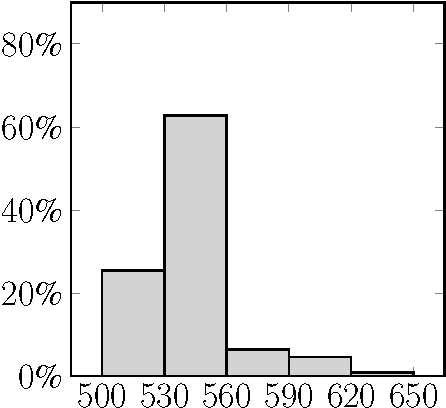
\includegraphics[width=0.97\linewidth]{histo-stage1-latency.pdf}\\
\begin{captext}
\centering
Mean: 541~$\pm$22~ms\hspace{0.1in}p99: 620~ms\\
\end{captext}
\vspace{-0.05in}
{\small (a) Latency (ms)}
\end{minipage}
\begin{minipage}[b]{0.49\linewidth}
\centering
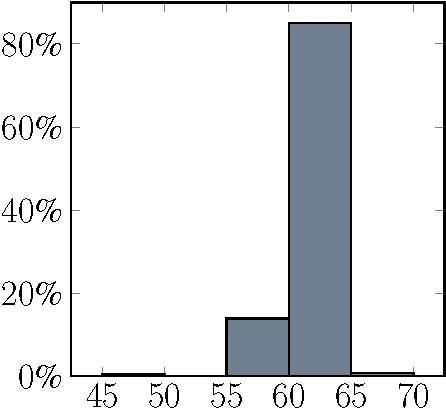
\includegraphics[width=0.97\linewidth]{histo-stage1-throughput.pdf}\\
\begin{captext}
\centering
Mean: 62~$\pm$1.5~fps\hspace{0.1in}p1: 59~fps\\
\end{captext}
\vspace{-0.05in}
{\small (b) Instant. Throughput (fps)}
\end{minipage}
\vspace{-0.15in}
\caption{\small Original FFmpeg-based Stage-1 Performance}
\label{fig:stage1-histo}
\vspace{-0.1in}
\end{figure}


Figure~\ref{fig:stage1-histo} presents our measurements of Stage-1. We
were surprised by the magnitude of the latency, with a mean of 541~ms.
Our cloudlet has two Intel Xeon processors with a total of 36 cores,
128GB of RAM and an NVIDIA GeForce GTX 1080 Ti GPU. This should be
ample for efficient software decoding of an H.264 video stream, as
confirmed by the mean throughput of 62~fps shown in
Figure~\ref{fig:stage1-histo}(b).  The high latency observed has no
obvious explanation, but it has a large negative impact on the
\ooda~pipeline.  As detailed elsewhere~\cite{Chanana2024}, we
determined that the culprit was negative latency scaleout of FFmpeg
when performing single stream
decoding~(Figure~\ref{fig:ffmpeg-threads-box-plot2}).

By switching to  different decoding software~\cite{PDrAW2024}, we
were able to reduce the latency from a mean of 541~ms in
\Cref{fig:stage1-histo}(a) to a mean of 32~ms in
\Cref{fig:pdraw-histo}(a).  This has been achieved with a mean
throughput of 37~fps~(\Cref{fig:pdraw-histo}(b)), which is well above
the demand of 31~fps from Observe$_{ab}$.  Assuming negligible
processing in Stage-2 and Stage-3, Figure~\ref{fig:pdraw-histo} shows
the best-case latency and throughput of Orient+Decide$_d$.

\begin{figure}
\centering
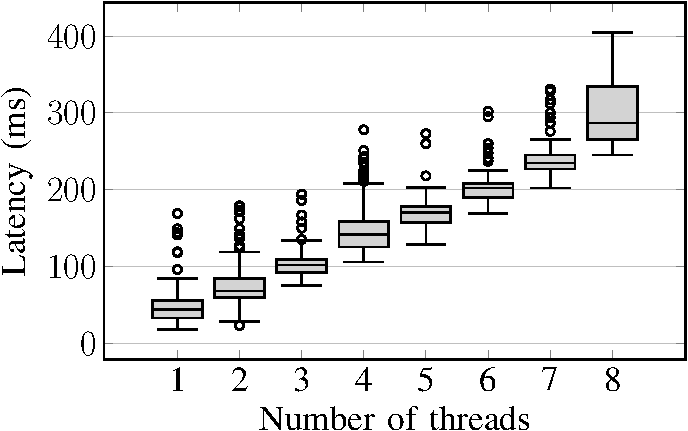
\includegraphics[width=0.75\linewidth]{histo-multi-threaded-ffmpeg.pdf}
\begin{captext}
  Each box extends from the first quartile ($Q_1$) to the third
  quartile ($Q_3$), with a line at the median. Whiskers extend from
  the box to the farthest data point lying within 1.5x the
  inter-quartile range ($IQR = Q_3-Q_1$) from the box. Circles
  represent outliers.
\end{captext}
\vspace{-0.1in}
\caption{\small Negative Scale-out of FFmpeg Latency}
\label{fig:ffmpeg-threads-box-plot2}
\end{figure}


\begin{figure}
\centering
\begin{minipage}[b]{0.49\linewidth}
\centering
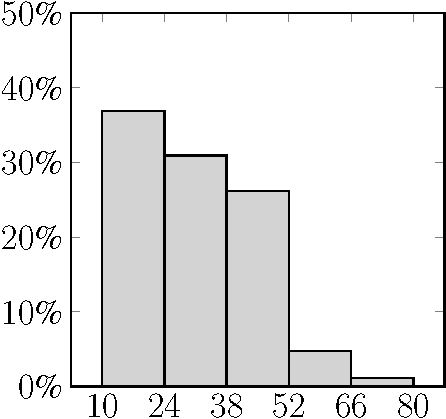
\includegraphics[width=0.97\linewidth]{histo-pdraw-latency.pdf}\\
\begin{captext}
\centering
Mean: 32~$\pm$13~ms\hspace{0.1in}p99: 59~ms\\
\end{captext}
{\small (a) Latency (ms)}
\end{minipage}
\begin{minipage}[b]{0.49\linewidth}
\centering
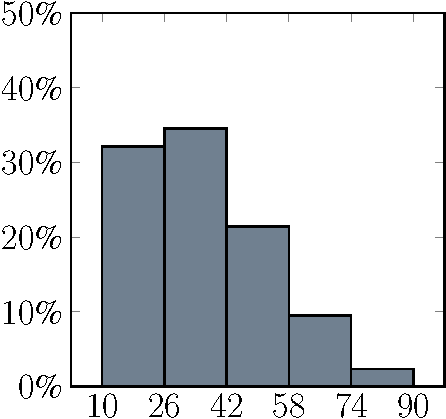
\includegraphics[width=0.97\linewidth]{histo-pdraw-throughput.pdf}\\
\begin{captext}
\centering
Mean: 37~$\pm$16~fps\hspace{0.1in}p1: 17~fps\\
\end{captext}
{\small (b) Instant. Throughput (fps)}
\end{minipage}
\vspace{-0.1in}
\caption{\small Improved Performance With FFmpeg Alternative}
\label{fig:pdraw-histo}
\vspace{-0.1in}
\end{figure}

\begin{figure}
\centering
\begin{minipage}[b]{0.49\linewidth}
\centering
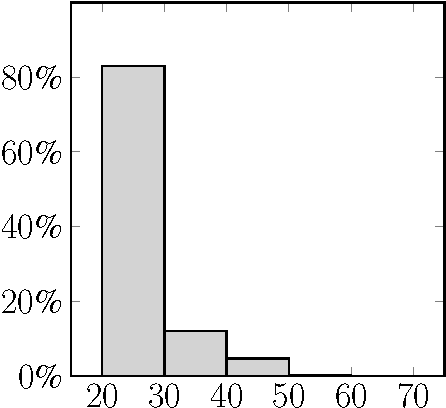
\includegraphics[width=0.97\linewidth]{histo-acte-latency.pdf}\\
\begin{captext}
\centering
Mean: 30~$\pm$4~ms\hspace{0.1in}p99: 49~ms\\
\end{captext}
{\small (a) Latency (ms)}
\end{minipage}
\begin{minipage}[b]{0.49\linewidth}
\centering
\includegraphics[width=0.97\linewidth]{histo-acte-throughput.pdf}\\
\begin{captext}
\centering
Mean: 28$\pm$3.7~Mbps p1: 19~Mbps\\
\end{captext}
{\small (b) Throughput (Mbps)}
\end{minipage}
\vspace{-0.15in}
\caption{\small Act${_e}$ Measurements}
\label{fig:c2d-net}
\end{figure}


\subsection{Act$_e$}
\label{sec:netuplink}

Figure~\ref{fig:c2d-net} presents our measurements of the wireless
network path from cloudlet to drone.  The latency has a mean of 30~ms,
with a standard deviation of 4~ms and a p99 of 49~ms.  The throughput
has a mean of 28~Mbps, with a standard deviation of 3.7~Mbps and a p1
of 19~Mbps.  Since no video is transmitted back to the drone, Act$_e$
is not a bottleneck.


\subsection{Act$_{fg}$}
\label{sec:c2d-drone}

\begingroup
\setlength{\columnsep}{4pt}

Black box hardware and software on the drone seamlessly integrate
components (f) and (g).  All that is externally visible is a set of
commands that are accessible via the drone's SDK~\cite{Olympe2024}.
The processing of a command and initiation of actuation are integrated
into Act$_{fg}$ in Figure~\ref{fig:nomenclature}.
\begin{wrapfigure}[11]{r}{0.45\linewidth}
\vspace{-0.07in}
\centering
%\includegraphics[width=0.45\linewidth]{FIGS/act_latency.png}
    \begin{tabular}{@{}cc@{}}
\toprule
Run & Latency (ms)\\
\midrule
 1&188\\
 2&170\\
 3&162\\
 4&189\\
 5&155\\
\midrule
Mean& 173~{\small$\pm15$}\\
\bottomrule
\end{tabular}
\caption{\small Act$_{fg}$  Latency}
\label{fig:c2d-drone-histo}
\vspace{-0.1in}
\end{wrapfigure}
In this context, latency corresponds to the time difference between
the receipt of an actuation command by the drone, and the start of
actuation.  To measure this difference, we position the stationary
drone in front of a display connected to the cloudlet.  The display
shows the current timestamp in milliseconds. We send a command to the
drone to move its camera gimbal, while recording the display and
gimbal using a slow-motion video camera. In post-processing, we
manually identify the timestamp of the command and that of the first
video frame showing gimbal movement.  Act$_{fg}$ latency is the
difference between these two timestamps.  Our slow-motion camera
operates at 240 fps, resulting in a frame interval of
\textasciitilde4~ms.  Our measurement has an error margin of
\textasciitilde5 frames, translating to experimental error of
\textasciitilde20~ms.

\endgroup

Figure~\ref{fig:c2d-drone-histo} presents our measurements.  The
latency distribution has a mean of 173~ms, with a standard deviation
of 15~ms.  Electromechanical actuation is far slower than processing
or network transmission, and there is no concept of streaming.  Our
benchmarks do not involve any back-to-back actuations without
intervening sensing and processing. Hence, throughput is best
interpreted as the reciprocal of latency.


\begin{figure}
\includegraphics[width=1.0\linewidth]{FIGS/fig-ooda-scaling.pdf}
\begin{captext}
  This figure uses the same notation as Figure~\ref{fig:nomenclature},
  and color coding as Figure~\ref{fig:ooda-loop}.  Width is scaled to
  represent latency, and height to represent throughput.
  Orient+Decide$_d$ here assumes negligible application-specific
  processing.  For the electromechanical actuation represented by
  component Act$_{fg}$, the reciprocal of its latency is used as its
  throughput.
\end{captext}
\vspace{-0.1in}
\caption{\small \ooda~ Loop Latency \& Throughput}
\label{fig:ooda-scaling}
\vspace{-0.1in}
\end{figure}

\subsection{The Full \ooda~Loop}
\label{sec:e2e-discussion}

Using the same notation as Figure~\ref{fig:nomenclature}, a visual
summary of the measurements reported in \S\ref{sec:d2c-drone} to
\S\ref{sec:c2d-drone} is shown in Figure~\ref{fig:ooda-scaling}.  This
captures the best-case \ooda~loop, where no time is spent in Stage-2
and Stage-3 of Orient+Decide$_d$.  In practice, it is those stages that
perform the processing for drone autonomy such as object detection,
object tracking, Kalman filtering, and route planning.  They also do
the processing to generate the commands for drone actuation such as
gimbal movement, flight path alteration, or altitude change.  The
height and width of the resulting Orient+Decide$_d$ component in
Figure~\ref{fig:ooda-scaling} would need to be scaled to include such
application-specific processing.  In some cases, that component
may dominate the entire \ooda~loop.

In a typical application, many iterations of the \ooda~loop may
involve no actuation, thus eliminating Act$_{e}$ and Act$_{fg}$.  For
example, consider a target that is moving in a straight line at
constant speed.  Successive \ooda~loops of a drone that is following
that target only need to confirm that it remains centered in the FOV.
Only abrupt change of motion by the target will stress the \ooda~loop.
Fast reaction is then needed to discover that the target is
off-center, and to actuate the gimbal or drone to re-center it before
it is lost from the FOV.  Figure~\ref{fig:ooda-scaling} shows that the
latency and throughput of Observe$_{ab}$ are the limiting constraint
in uneventful settings.  It is thus the inherent attributes
of the drone, rather than network bandwidth or the cloudlet processing
power, that limits us today.

\begin{comment}
\begin{figure}
\centering
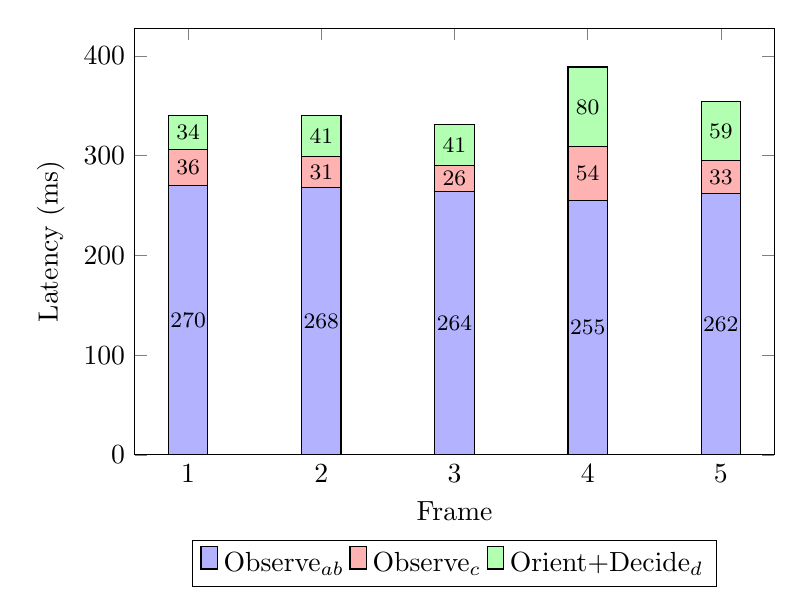
\begin{tikzpicture}
    \begin{axis}[
        ybar stacked,
        bar width=0.5cm,
        width=0.8\linewidth,
        height=7cm,
        ylabel={Latency (ms)},
        xlabel={Frame},
        symbolic x coords={1, 2, 3, 4, 5},
        xtick=data,
        ymin=0,
        legend style={at={(0.5,-0.2)},
                      anchor=north,legend columns=3},
        nodes near coords,
        every node near coord/.append style={font=\footnotesize, /pgf/number format/.cd, fixed, precision=1},
    ]
        \addplot+[ybar, color=black, fill=blue!30] plot coordinates {(1, 270) (2, 268) (3, 264) (4, 255) (5, 262)}; % Oberve_ab
        \addplot+[ybar, color=black, fill=red!30] plot coordinates {(1, 36) (2, 31) (3, 26) (4, 54) (5, 33)}; % Observe_c
        \addplot+[ybar, color=black, fill=green!30] plot coordinates {(1, 34) (2, 41) (3, 41) (4, 80) (5, 59)}; % Orient+Decide_d

        \legend{Observe$_{ab}$, Observe$_c$, Orient+Decide$_d$}
    \end{axis}
\end{tikzpicture}
\vspace{-0.1in}
\caption{\small{Latency Breakup by {\sc OODA} phase}}
\label{fig:latency-breakup}
\end{figure}

% If we show this stacked bar chart in terms of averages instead of the
% breakup for five example frames we can include the Act phase as well.
%
% So then there would be just one bar in the stacked bar chart.
\end{comment}



\chapter{Benchmarking the SteelEagle Pipeline}
While the \ooda~loop provides a broad understanding of drone reaction time, it does little to measure agility in real-world flight operations. In practice, it is performance on the latter that actually matters. Unfortunately, measuring this performance is difficult because there is no existing metric that defines the units in which to express an answer.

Agility is a complex emergent cyber-physical property that depends
both on cyber properties such as latency, throughput, and accuracy of
the \ooda~loop, as well as physical properties such as the drone's
size, weight, thrust, lift, drag and moment of inertia.  Under benign
conditions, a non-agile drone may do as well as an agile one.  Only
under adversarial conditions does the cost of agility become valuable.
This cost may include increased size, weight, and bandwidth/latency
demand arising from the need to be faster and more accurate in sensing
and actuation.  The only way to quantify this complex property is to
stress a drone on a precisely-defined task in a reproducible
environment, and to use task-level metrics as surrogates for agility.
This leads directly to the creation of benchmarks for evaluating
autonomous drone agility.

In this chapter, I define two agility benchmarks for measuring drone agility. The first benchmark embodies tracking of an object that moves in an unpredictable manner, with many abrupt changes. The adversarial aspect of this benchmark lies in the existence of an active mobile agent that randomly changes its trajectory. The second benchmark embodies obstacle avoidance in tight spaces. The adversarial aspect of this benchmark lies in the close proximity of obstacles, the need to sense them in real time (e.g., to account for wind effects), and occlusion that prevents full foreknowledge of the optimal flight path.  Both benchmarks are parameterized, thereby enabling many levels of difficulty within a common benchmark framework. In Section~\ref{sec:prior-work-benchmarks}, I discuss previous work related to real drone flight benchmarking in reactive scenarios, and how my work improves upon it. In Section~\ref{sec:avoidance}--\ref{sec:tracking-results}, I outline my benchmarks for object tracking and obstacle avoidance respectively and the results from my experiments using them.

\section{Prior Work on Drone Benchmarks}
\label{sec:prior-work-benchmarks}

There have been many efforts in the computer vision and machine
learning community to create benchmarks for comparing drone
performance on specific tasks. These focus exclusively on the accuracy
of algorithms such as drone-based object tracking and face
recognition, ignoring system attributes such as agility and end-to-end
processing latency. Du et al~\cite{Du2018}, Li et al~\cite{Li2017},
Kalra et al~\cite{Kalra2019}, and Zhao et al~\cite{Zhao2024} are
examples of this genre.

Many drone benchmarks do measure agility but involve only simulated
tests. MAVBench~\cite{Boroujerdian2018} is one popular example. It
consists of a closed-loop simulator and end-to-end application
benchmark suite of five workloads pertaining to scanning, aerial
photography, package delivery, 3D Mapping, and Search and Rescue.
These workloads lack customization options, and often represent a
specific simulated scenario which can only give limited perspective on
real performance. Another simulation-based benchmark,
FlightBench~\cite{Yu2024}, has agility workloads which provide several
levels of difficulty. However, this difficulty is determined
arbitrarily by the authors and the obstacle courses are too complex to
practically replicate outside of the simulator. Additionally,
simulations typically do not fully capture real flight performance,
where sensors can experience noise which can influence actuation.

There are live flight drone benchmarks that measure agility, but they
are not as common. One example is the disturbance benchmark proposed
by Wu et al~\cite{Wu2021} which uses an indoor course along with a fan
to emulate obstacle avoidance in windy conditions. The course is fixed
and does not provide guidance for replicating the described
experiments. For this reason, while it is useful for evaluating the
paper's proposed trajectory planner, it is not as useful for measuring
the performance differences between different avoidance methods.

Koubaa et al~\cite{Koubaa2020} describe an experimental study that
compares on-board drone processing versus offloading to the cloud. The
metrics of interest in their work are energy cost, bandwidth demand,
and timeliness of results.  The last of these metrics is closest to
our focus on the agility of drones.  However, the experiments
described do not include drone actuation in response to real-time
observations.  They are purely open loop experiments, with timeliness
to cloud users being the metric of interest.  Further, this work only
provides micro-benchmarks to evaluate these metrics.  There are no
end-to-end benchmarks that include the full \ooda~pipeline of
sensing, processing and drone actuation.

Beyond these experimental efforts is a vast body of published
literature on analytical or simulation-based evaluations of algorithms
for specific drone tasks.  Examples include the work of Chen et
al~\cite{Chen2020}, Hayat et al~\cite{Hayat2021}, Wang et
al~\cite{Wang2020}, and Wu et al~\cite{Wu2020}.  These studies
abstract away the physical drone, relying instead on hypothetical cost
models of processing and communication.  AdaDrone~\cite{Chen2022} is a
slightly more realistic approach that leverages a drone simulator.
None of these efforts use real drones, with their intrinsic
limitations of weight and maneuverability.  In contrast to these prior
works, I focus on providing
\textit{parameterized} and \textit{reproducible} benchmarking of
drones in actual flight.


\section{Visual Object Tracking: Benchmark}
\label{sec:tracking}
In visual object tracking, a drone follows a moving target and tries
to keep it centered in its FOV.  Many surveillance-related instances
of this task, where the target may be adversarial and actively try to
escape tracking, occur in law enforcement and military settings.  The
task is also relevant to wildlife conservation research, where an
animal of an endangered species is identified and followed in the
wild.  It is also used in filmmaking to capture evolving scenes.  In
such use cases, using an autonomous drone for tracking could reduce
attention demand on mission personnel.

\subsection{Benchmark Requirements}
\label{sec:tracking-requirements}

The size and visual appearance of a target plays an important role in
tracking success.  An object that is just a few pixels in size from
the altitude of the drone will be inherently difficult to
detect~\cite{Huang2017}.  Poor contrast with the background, as
happens when camouflaged, also contributes to poor detection.  Objects
that are hard to detect are also hard to track, since actuating to
re-center the target in each frame is key to success.  The object
being tracked and the background on which it moves both need to be
specified.  Only when these factors and drone optics are held
constant will \ooda~loop performance come to the fore in determining
tracking performance.

The other benchmark requirements for tracking are similar to those
described for obstacle avoidance~(\S\ref{sec:avoidance-requirements}).
Parameterization that controls the difficulty of the task is valuable.
Use of standardized, off-the-shelf components and careful attention to
reproducibility of results are important.

\subsection{Benchmark Description}
\label{sec:tracking-description}
The object followed in my tracking benchmark is a DJI Robomaster S1
robot~\cite{Robomaster2022} as in Section~\ref{sec:task3}.  Tracking is done on a level, green background such as a football field.  For this combination of target and background, DNN-based object detection from an altitude of 10~m is successful at a confidence level of 0.9 or higher on frames from my drone's video camera.

My benchmark is a random walk with turns in a randomly-chosen
cardinal direction at each step.  Figure~\ref{fig:tracking-path}(a)
shows one example with 5 steps, and Figure~\ref{fig:tracking-path}(b)
shows other examples with more steps.  The benchmark has three
parameters: the number of steps;  the mean length of each step;
and the target speed of 1.5~m/s, 2.5~m/s, or 3.5~m/s.  The
benchmark could be made more complex by making the turns to be at any
angle rather than just cardinal directions, and by making step size
and target speed non-uniform.  All my experiments were conducted
across the full range of speeds, using a stepcount of 35 steps
and stepsize  set to 5~m.

\begin{figure}
\centering
\begin{minipage}{0.6\linewidth}
\centering
\includegraphics[width=0.8\linewidth]{chapter6/FIGS/fig-tracking-onepath.png}\\
{(a) Detail for 5-Step Example}
\end{minipage}
\begin{minipage}{0.35\linewidth}
\centering
\includegraphics[width=0.35\linewidth]{chapter6/FIGS/fig-tracking-manypaths.png}\\
{(b) Other Examples}

\end{minipage}
\caption{Parameterized Random Walk}
\label{fig:tracking-path}
\end{figure}


To execute the benchmark, the target is placed in a large open outdoor
area.  The drone is manually piloted to the desired altitude, and its
FOV is adjusted to center the target. Once the drone has locked
onto its target, the target is instructed to start its pre-programmed
random walk and a timekeeper starts a stopwatch. The experiment
continues until one minute has elapsed or the drone loses the target
from its FOV.  The termination time and the black box footage of the
flight are logged for post-flight
scoring~(\S\ref{sec:tracking-scoring}).

\begin{figure}
\centering
\begin{minipage}{0.35\linewidth}
\centering
\includegraphics[width=\linewidth]{chapter6/FIGS/fig-tracking-scoring.png}
\caption{\small $\vec{O}$ \& $\vec{D}$}
\label{fig:o-d-calc}
\end{minipage}
\begin{minipage}{0.5\linewidth}
\small
\begin{equation}
	c_i = \norm{\vec{O}_i} / \norm{\vec{D}_i}\label{eq:2}
\end{equation}
\begin{equation}
	s_{i} = 1.1^{-c_i}\label{eq:3}
\end{equation}
\begin{equation}
	s_{\text{avg}} = \frac{\Sigma_i^n s_i}{n}\label{eq:4}
\end{equation}
\caption{Calculating Score\\[0.2cm]}
{\centering\small
$\norm{\vec{O}} = 0.11$, $\norm{\vec{D}} = 0.03$, $c = 3.67$ \\[0.1in]
$s_{10} = 1.1^{-c} = 0.70$ \\
$s_{20} = 1.2^{-c} = 0.51$ \\
$s_{30} = 1.3^{-c} = 0.38$ \\
}
\caption{Scoring Figure~\ref{fig:track-score-example}}
\label{fig:example-score-calcuclation}
\end{minipage}
\end{figure}

\begin{figure}
\centering
\includegraphics[width=0.9\linewidth]{chapter6/FIGS/fig-tracking-score-demo.png}
\caption{Example Frame for Scoring}
\label{fig:track-score-example}
\end{figure}

\subsection{Benchmark Scoring}
\label{sec:tracking-scoring}
In post-processing after a flight, I score the recorded video footage
using an automated process.  Figures~\ref{fig:o-d-calc} to
\ref{fig:example-score-calcuclation} show the scoring calculation,
using Figure~\ref{fig:track-score-example} as an example.  On each
frame, a DNN is first used to create a bounding box around the target.
With the center of the frame as the origin, the relative distance of
the target from the origin is obtained.  Using the notation shown in
Figure~\ref{fig:o-d-calc}, the pixel offset vector, $\vec{O}$, gives
the L2 distance of the target's centroid from the origin.  This is scaled
to the vector dimension, $\vec{D}$, of the bounding box to give the
centering ratio $c_i$~(formula \ref{eq:2}).  I then calculate the
score of the frame, $s_i$, by using an inverse exponential, as shown
in formula~\ref{eq:3}.  The rationale for using an exponential is to
super-linearly penalize distance from origin.  I use a compounding
10\% penalty in reporting my results, leading to the value of 1.1 in
formula~\ref{eq:3}.  Using $s_n$ to denote a penalty of n\%,
Figure~\ref{fig:example-score-calcuclation} shows the scores for
penalties of 10\%, 20\% and 30\% for the example frame in
Figure~\ref{fig:track-score-example}.  A score of zero is awarded when
the frame does not contain the target at all, or if the target is too
small to be detected in post-processing by a specified model.  In my
case, this model is YOLOv5x trained on aerial images of the target.

From the per-frame scores, the entire flight is scored by simple
averaging ~(formula \ref{eq:4}). The overall score, $s_{\text{avg}}$,
lies between $0$ and $1$, with higher being better. For
example, an average score of $0.70$ based on $s_{10}$ is achieved when
the drone is able to keep the target within about three normalized
lengths of the center of the FOV for the entire duration of the
flight.

\begin{table}
\centering
\begin{tabular}{|l|c|c|c|}
\hline
\textbf{Model} & \textbf{Latency} & \textbf{Throughput} & \textbf{mAP} \\
 & (ms) & (fps) & \\
\hline
YOLOv5s  & 28 & 25 & 56.8\\
YOLOv5m  & 37 & 20 & 64.1\\
YOLOv5l  & 42 & 20 & 67.3\\
\hline
\end{tabular}
\begin{captext}
  \\[0.1cm] \small The inference and throughput were obtained on the
  cloudlet~(\S\ref{sec:cloudlet}).  The mean average precision~(mAP)
  is from the YOLO documentation~\cite{Yolo}.
\end{captext}
\caption{YOLOv5 Performance in the SteelEagle Pipeline}
\label{fig:yolo-model-stats}
\end{table}


\subsection{Tracking Algorithm}
\label{sec:tracking-algorithm}
For this benchmark, I use the tracking algorithm used described in Section~\ref{sec:tracking-algorithm-advanced}. Figure~\ref{fig:yolo-model-stats} shows the latency, throughput and
accuracy of the three DNN models that are used for tracking in my
system, each trained on the Robomaster target.  Even using the slowest of these as Stage-2 of
Orient+Decide$_d$ only adds 42 milliseconds of latency to the base
value of 527~ms~(Figure~\ref{fig:ooda-scaling}).  Its throughput of
20~fps is well above that of the bottleneck~(Act$_{fg}$).  However,
there may be situations where load on a multi-tenant cloudlet may need
to be reduced, and the smaller models may be valuable for that
purpose.

\section{Visual Object Tracking: Results}
\label{sec:tracking-results}
The basic question I ask about tracking is as follows:
\begin{itemize}
\item{\em How well does my platform follow a target that makes random,
  rapid changes in direction?}
\end{itemize}
As Figure~\ref{fig:tracking-best} shows, my platform is able to track
the target on my benchmark even at the fastest speed~(3.5~m/s)
without ever completely losing it.  However, as the scores show, the
target is off-center in some frames at all speeds.  As target speed
decreases, the score achieved shows a modest improvement.  The results
shown here are based on the best model for each speed.  This
dependence is explored further in \S\ref{sec:tracking-models}.

\begin{figure}
\centering
\begin{minipage}{0.49\linewidth}
\centering
\includegraphics[width=1.0\linewidth]{chapter6/FIGS/fig-tracking-best.pdf}\\
\caption{Baseline Scores}
\label{fig:tracking-best}
\end{minipage}
\begin{minipage}{0.49\linewidth}
\centering
\includegraphics[width=1.0\linewidth]{chapter6/FIGS/fig-tracking-human.pdf}\\
\caption{Human Pilot}
\label{fig:tracking-human}
\end{minipage}
\end{figure}

As in the case of obstacle avoidance, I ask how well an experienced
human pilot performs under identical conditions. The pilot is held
constant from \S\ref{sec:avoidance}.
Figure~\ref{fig:tracking-human} shows how well the human pilot scored
on the benchmark.  Comparing Figures~\ref{fig:tracking-best} and
~\ref{fig:tracking-human}, I see that the autonomous drone and the
human are comparable at 1.5~m/s, but at higher speeds the autonomous
drone outperforms the human.  This is in contrast to obstacle
avoidance~(Figures~\ref{fig:avoid-best} and \ref{fig:avoid-human}),
where the human consistently outperformed the autonomous drone.  I
conjecture that at least part of this difference is attributable to
the fact that the obstacle course is static, and hence subconscious
pre-planning by the human helps in navigating it.  In contrast, the
human is no better than the drone in anticipating random turns made by
the target.  At higher speeds, raw reaction speed~(i.e., the
\ooda~loop) is all that matters, and the autonomous drone proves to be
better in this regard.

\begin{figure}
\centering
\includegraphics[width=0.8\linewidth]{chapter6/FIGS/fig-tracking-models.pdf}
\caption{\small Impact of YOLO Model on Tracking Benchmark}
\label{fig:track_models}
\end{figure}

\subsection{Impact of Model Accuracy}
\label{sec:tracking-models}

Since multiple DNN models are available to use in
tracking~(Figure~\ref{fig:yolo-model-stats}), I ask the following
question:
\begin{itemize}
\item{\em Does the use of a better model improve tracking?}
\end{itemize}
Figure~\ref{fig:track_models} presents my results.  For any given
speed, there is little difference across models.  The increased
cloudlet load of a more accurate model does not pay off.  However, it
should be noted that this observation may only be true for this
specific tracking benchmark.  As described
in~\S\ref{sec:tracking-description}, the benchmark is defined as being
conducted in an open area free of clutter.  If I were to create a
different tracking benchmark that embodies extensive clutter~(such as
that of a busy street filled with moving cars, bicycles, and
pedestrians, along with static objects such as parked cars and trees),
the results may be quite different. In that case, the improved
accuracy of the larger models may prove decisive. The creation of such a benchmark could be a subject of future work.

\begin{figure}
\centering\small
\begin{minipage}{0.8\linewidth}
\centering
\includegraphics[width=0.98\linewidth]{chapter6/FIGS/fig-tracking-latency.pdf}\\
(a) Additional Latency
\end{minipage}
\begin{minipage}{0.8\linewidth}
\centering
\includegraphics[width=0.98\linewidth]{chapter6/FIGS/fig-tracking-fps.pdf}\\
(b) Reduced Throughput
\end{minipage}
\caption{Impact of Latency and Throughput on Tracking}
\label{fig:tracking-latency-throughput}
\end{figure}

\subsection{Impact of Latency \& Throughput}
\label{sec:tracking-factors}

As in the case of obstacle avoidance~(\S\ref{sec:avoidance-factors}),
I ask:
\begin{itemize}
\item{\em What is the impact of latency or throughput degradation of
    the \ooda~loop on benchmark score?}
\end{itemize}
Figure~\ref{fig:tracking-latency-throughput}(a) shows what happens
when additional latency of 250~ms and 500~ms are added to the
\ooda~loop.  For all target speeds and models, there is a noticeable
drop in benchmark score.  The drop is worse at higher speeds.  This is
directly attributable to the inability of the more sluggish \ooda~loop
to keep the target centered in the FOV.  At higher speeds, the drone
often loses sight of the target early in the tracking.  This results
in a zero score for the remaining frames of that experiment, and hence
an overall low average score.

Figure~\ref{fig:tracking-latency-throughput}(b) shows the same trend
when \ooda~loop throughput is artificially throttled to 3~fps or
1~fps.  At all target speeds and for all models, there is a noticeable
drop in benchmark score.  This drop is greater at higher speeds.

The results in Figures~\ref{fig:tracking-latency-throughput}(a) and
(b) confirm that both end-to-end latency and bottleneck throughput are
important independent factors in determining tracking ability.
Optimizing one at the cost of the other, as occurs when using
strategies such as batching of operations, is unlikely to be
beneficial.


\section{Obstacle Avoidance: Benchmark}
\label{sec:avoidance}
Obstacle avoidance is vital for drone flights at low altitude (up to a
few hundred feet) in urban or forested settings. Otherwise, being restricted to only high altitude flight impairs visual detections and hides many details.  The most dangerous obstacles are
typically trees, lightposts, and telephone poles, which can easily
reach altitudes usually used by drones. Being  relatively thin,
they are difficult to detect from afar.  

Efficient avoidance of such obstacles is a challenge.  Since drone
flight is limited by battery life (typically on the order of 30-50
minutes), bypassing obstacles without wasting too much flight time is
important. If flight is too slow or avoidance maneuvers are too
convoluted, mission performance will be impaired.  At the same time,
reckless flight could be catastrophic.  Striking the right balance
between safety and speed for the given flight conditions is essential.
Since effective but rapid avoidance of obstacles is a valuable
capability in a drone, this task is a good candidate for an agility
benchmark.

\subsection{Benchmark Requirements}
\label{sec:avoidance-requirements}

A good benchmark for this task should capture the essential difficulty
of obstacle avoidance.  It should be parameterized, so that it is easy to
vary the difficulty of the benchmark.  The benchmark should only use
standardized, off-the-shelf components that can be easily purchased or
fabricated.  There should be no ambiguity in the experimental setup or
interpretation of results, thereby simplifying independent attempts to
reproduce published experimental results.
\S\ref{sec:avoidance-description} presents my candidate benchmark
that meets these requirements.

\subsection{Benchmark Description}
\label{sec:avoidance-description}

\begin{figure}
    \centering
    \includegraphics[trim=-4cm 0 0 0, width=0.5\linewidth]{chapter6/FIGS/fig-obstacle-course.png}
    \caption{Obstacle Course Layout}
    \label{fig:obstacle-course}
\end{figure}

To emulate tall and skinny obstacles such as lightposts, I use 1.8~m
long drone racing flags.  The flags are
arranged in a precisely-defined slalom
pattern~(Figure~\ref{fig:obstacle-course}), that forces a drone to
sequentially evade several obstacles.  The difficulty of the course is
controlled by a spacing parameter, $w$, that determines the separation
of the flags along both the azimuth and range axes.  A smaller value
of $w$ defines a more difficult course because of higher density of
obstacles in both directions.  All my experiments were conducted with
4 tiers of obstacles.  Adding more tiers to make the obstacle course
longer, while preserving obstacle spacing, would add further
difficulty to the course.  The drone's goal is to navigate the course
as fast as possible, without touching the flags or striking a
flagpole.  The metric of interest is the transit time through the
course.

To execute this benchmark, the obstacle course is set up as in
Figure~\ref{fig:obstacle-course}.  The drone is placed on a pad that
is centered 4~m in front of the leading line of flags.  A human
spotter stands a safe distance behind the drone, and a human
timekeeper is positioned along the finish line.  The remote
pilot-in-command (RPIC) continuously monitors the video stream from
the drone, and stands ready to wrest back manual control if the
drone's autonomous flight software appears to be getting it into
trouble.  Such a manually aborted flight is scored as ``Did Not
Finish~(DNF).''  A flight in which the drone touches a flag
or pole is also scored as DNF.

The drone takes off and then hovers at an altitude of 1~m.  It
is then directed to autonomously move to a destination beyond the
obstacle course. When forward motion begins, the spotter visually
signals the timekeeper to start a stopwatch. The spotter then follows
the drone through the course, warning the RPIC of imminent collision,
if any.  Such a warning aborts the experiment without damage to the
drone.  On a successful flight, timing is stopped as soon as the
trailing end of the drone crosses the finish line.  We deem an
obstacle spacing, $w,$ as viable if the drone successfully flies
through the course on at least 80\% of its attempts.  The average time
of these successful flights at the smallest viable $w$ is the figure
of merit. For small values of $w$, a more agile drone can fly more
aggressively and therefore requires less time to complete the benchmark.
However, at higher values of $w$, agility may not be important because
the obstacle course easier.

\begin{table}
\small
	\centering
        \begin{tabular}{|c|c|c|}
		\hline
		\textbf{Model} & \textbf{Latency (ms)} & \textbf{Throughput (fps)} \\
		\hline
		MiDaS Small & 61 & 10 \\
		DPT Hybrid & 105 & 8 \\
		DPT Large & 132 & 7 \\
		\hline
	\end{tabular}
\begin{captext}
\centering
    \\[0.1cm]
  \small These numbers were obtained on the cloudlet described in
  \S\ref{sec:cloudlet}
\end{captext}
\caption{Inference Speeds of MiDaS DNN Models}
\label{tab:midas-model-stats}
\end{table}

\subsection{Benchmark Scoring}
\label{sec:avoidance-scoring}

The average time, $t_{\text{avg}}$, for multiple experimental runs at
the lowest viable $w$ is a raw measure of agility.  However, this needs
to be normalized with respect to attributes other than agility.
For example, a drone whose top speed is low relative to other drones
may be penalized unfairly when measuring agility.  A low value of
$t_{\text{avg}}$ in that case is not due to a poor \ooda~loop, but
simply reflects the ``brute force'' attribute of top speed.  The
normalization is performed by removing flags from the course and
conducting a control experiment at top speed.  We denote the average
time for multiple runs of the control experiment as $t_{\text{min}}$.
The score, $S_w$, is then given by:
\begin{equation}
	S_w = \frac{t_{\text{min}}}{t_{\text{avg}}}\label{eq:1}
\end{equation}
Scores for this benchmark thus lie in the interval $0 < S_w \leq 1$
where $S_w = 1$ is the best possible score. A score of 0 is awarded
when a drone cannot achieve a successful completion rate of at least
80\% of the runs for the given value of $w$.

\subsection{Depth Sensing}
\label{sec:midas}

I use the same MiDaS-based avoidance algorithm described in Section~\ref{sec:midas-algorithm}. For this task, the \ooda~loop determines the speed and accuracy with which the drone can acquire fresh frames, execute the MiDaS algorithm on them, calculate new headings for safety, and perform actuations towards those headings.  In the context of \S\ref{sec:cloudlet}, MiDaS represents Stage-2 of cloudlet processing.  Stage-3 is the processing of MiDaS output to determine a new heading, and generating the actuation command. Figure~\ref{fig:midas-sample-course} shows the algorithm running on a setup benchmark course.

\begin{figure}
	\begin{minipage}{0.495\linewidth}
		\centering
		\includegraphics[width=0.8\linewidth]{chapter6/FIGS/fig-obstacle-course-drone-pov.jpg}\\
		{(a) Raw Input}\\
	\end{minipage}
	\begin{minipage}{0.495\linewidth}
		\centering
		\includegraphics[width=0.8\linewidth]{chapter6/FIGS/fig-obstacle-course-midas.jpg}\\
		{(b) Output of MiDaS}\\
	\end{minipage}
\caption{MiDaS Running on the Benchmark Course}
\label{fig:midas-sample-course}
\end{figure}

I explore three DNN variants of MiDaS that vary in accuracy and speed:
{\em MiDaS Small,} {\em DPT Hybrid}, and {\em DPT Large}.  MiDaS Small
prioritizes throughput and inference latency at the cost of lower
accuracy. DPT Hybrid strikes a compromise between speed and accuracy.
DPT Large prioritizes accuracy above all else.  Figure
\ref{tab:midas-model-stats} shows the inference latency and throughput
of these three models on my cloudlet.  I explore the use of all three in my experiments.


\section{Obstacle Avoidance: Results}
\label{sec:avoidance-results}
The most basic questions in my evaluation are as follows:
\begin{itemize}
\item{\em What is the smallest value of $w$ for which the drone can
    successfully complete the benchmark?}

\item{\em At that $w$, how fast is benchmark completion?}

\item{\em As $w$ is increased, how much faster is the drone able to
    complete the benchmark?}
\end{itemize}

Initial experiments showed that 2~m is the smallest value of $w$
that meets my criterion for successful benchmark completion (i.e., at
least 80\% of the flights are successful).  Using the scoring
criterion described in \S\ref{sec:avoidance-scoring},
Figure~\ref{fig:avoid-best} shows how well the drone
 did for $w$ set
to 2~m, 2.5~m, and 3.0~m.  The results shown are the mean of 5 runs of
each experiment.  For each value of $w$, the drone results were
obtained with the choice of MiDaS model that gave the best results.
These choices were DPT Large for $w = $2~m, and MiDaS Small for $w =
2.5$~m and $w = 3$~m.  The scores of 0.13 to 0.2 show that the drone
suffers almost an order of magnitude slowdown when avoiding obstacles,
relative to its unimpeded traversal of the course.  This is the price
of having to execute the \ooda~loop shown in
Figure~\ref{fig:ooda-scaling}, with the additional Stage-2 and Stage-3
processing for depth estimation described in \S\ref{sec:midas}.  As
$w$ is increased from 2~m to 3~m, Figure~\ref{fig:avoid-best} shows
the score improving from 0.13 to 0.2.  This confirms my expectation
that less challenging courses are faster to traverse.

Since humans are the standard against which AI systems are measured,
I ask how a human pilot does under identical conditions. To
explore this, an experienced RPIC with several dozen hours of flight
time on the Parrot ANAFI platform manually executed the benchmark for
the same values of $w$. The \ooda~loop is now cyber-human: the RPIC uses the drone's live video stream to manually fly it.  Of course, a human also
has foreknowledge of the obstacle course and can subconsciously
leverage that knowledge in planning the drone's flight.  In contrast,
the autonomous drone is purely reactive --- what it sees right now is
all that it knows.

Figure~\ref{fig:avoid-human} presents my results.  Relative to
unimpeded traversal of the course, the scores of 0.76 to 0.46 show
that even the RPIC suffers a slowdown.  However, the slowdown is much
smaller than that suffered by the autonomous drone in
Figure~\ref{fig:avoid-best}.  Since the drone hardware and wireless
network are identical in the two sets of experiments, the difference
is due to the superior \ooda~loop of the human.  There is
clearly ample headroom for improvement of the drone's \ooda~loop.

\begin{figure}
\centering
\begin{minipage}{0.45\linewidth}
\centering
\includegraphics[width=1.0\linewidth]{chapter6/FIGS/fig-avoidance-best.pdf}\\
\caption{Baseline Scores}
\label{fig:avoid-best}
\end{minipage}
\begin{minipage}{0.45\linewidth}
\centering
\includegraphics[width=1.0\linewidth]{chapter6/FIGS/fig-avoidance-human.pdf}\\
\caption{Human Pilot}
\label{fig:avoid-human}
\end{minipage}
\end{figure}


\begin{figure}
\centering
\includegraphics[width=0.8\linewidth]{chapter6/FIGS/fig-avoidance-models.pdf}
\caption{Impact of MiDaS Model on Avoidance Benchmark}
\label{fig:avoidance_by_model}
\end{figure}


\subsection{Impact of Model Accuracy}
\label{sec:avoidance-models}
The availability of the different MiDaS models shown in
Table~\ref{tab:midas-model-stats} leads to the question:
\begin{itemize}
\item{\em Is accuracy or speed  more important?}
\end{itemize}
My experiments indicate that there is no simple answer to this
question.  The results in Figure~\ref{fig:avoid-best} were
obtained using the best MiDaS model for each value of $w$.  MiDaS
Small performs the best on the 3~m course but worst on the 2~m course.
DPT Large is the inverse, performing best on the 2~m course and worst
on the 3~m course.  DPT Hybrid stays consistently in the middle for
all three courses.  The fact that different models had to be used in
each case to obtain the best results indicates that there is no single
``best'' model.  

I conducted a set of experiments to better understand this tradeoff
space.  The results in Figure~\ref{fig:avoidance_by_model} show the
score achieved on the benchmark for each model and value of $w$.
Since MiDaS Small focuses on throughput and low latency over accuracy,
a drone that uses it is able to sustain a higher maximum speed than
one using DPT Large.  At $w = $3~m, the course is sufficiently easy
that the increased risk of collision is small.  The higher accuracy of
a better model is not useful.  However, at $w = $2~m, the increased
likelihood of collisions makes higher model accuracy worthwhile.  Now,
DPT Large attains the highest score.  For a tight course, it is
difficult to travel at high speed without collisions. Hence, a model
that can navigate the gaps better gets a higher  score.

\begin{figure}
\centering
\begin{minipage}{0.8\linewidth}
\centering
\includegraphics[width=0.96\linewidth]{chapter6/FIGS/fig-avoidance-latency.pdf}
(a) Additional Latency
\end{minipage}
\begin{minipage}{0.8\linewidth}
\centering
\includegraphics[width=0.96\linewidth]{chapter6/FIGS/fig-avoidance-fps.pdf}
(b) Reduced Throughput
\end{minipage}
\caption{Impact of Latency and Throughput on Avoidance}
\label{fig:avoidance-latency-throughput}
\end{figure}

\subsection{Impact of Latency \& Throughput}
\label{sec:avoidance-factors}

The results presented so far reflect best-case conditions.  In
practice, the wireless network or the cloudlet may suffer degradation
due to multi-tenancy.  This leads to the question:
\begin{itemize}
\item{\em What is the impact of latency or throughput degradation of
    the \ooda~loop on benchmark score?}
\end{itemize}
The baseline scores reflect what is
achievable with an \ooda~loop whose latency is the sum of three
components:
\begin{itemize}
\item{a lower bound of 527~ms~(Figure~\ref{fig:ooda-scaling}).}

\item{the latency of the relevant MiDaS model~(Table~\ref{tab:midas-model-stats}).}

\item{a small additional overhead ($<$1~ms) for Stage-3 processing
    in the Decide part of the \ooda~loop.}
\end{itemize}

This total end-to-end latency is on the order of 600--650~ms.  For
\ooda~loop iterations that involve drone actuation, the bottleneck
throughput is the smaller of 6~fps for
Act$_{fg}$~(\S\ref{sec:c2d-drone}) and the throughput of the MiDaS
model~(Table~\ref{tab:midas-model-stats}).  This is effectively
6~fps, regardless of model.  If no drone actuation is involved, the
bottleneck throughput becomes that of the MiDaS model.  Since even
MiDaS Small has lower throughput than Observe$_{ab}$, Observe$_{c}$,
or best-case Orient+Decide$_d$, throughput is always in the 6--10~fps
range.

Figure~\ref{fig:avoidance-latency-throughput}(a) shows how benchmark
score drops as latency is artificially added to the \ooda \\ loop.  Even
250~ms of additional latency (i.e., a roughly 35--40\% increase from
baseline) causes benchmark score to drop to nearly half its baseline
value, for all values of $w$ and regardless of MiDaS model.  If 500~ms
of latency is added, the score drops further.  For the most
challenging course~($w = 2$~m), the score drops to zero because not
even 80\% of the flights are successful.  These results are consistent
with a long-standing design principle of deeply-immersive closed-loop
interactive systems: {\em increased latency is deadly, even if
  throughput remains good.}

Figure~\ref{fig:avoidance-latency-throughput}(b) shows how benchmark
score drops as the throughput of the \ooda~loop is artificially
reduced from its baseline value.  Reducing throughput to 3~fps causes
benchmark score to drop to nearly 40--50\% of its baseline value.  A
further drop is observed when throughput is reduced to 1~fps.  For $w
= 2$~m, the benchmark score drops to zero.  These results confirm that
latency is not the sole determinant of task performance in an
\ooda~loop --- throughput also matters.

\subsection{Value of On-board Drone Intelligence}
\label{sec:djiminipro}

Edge computing allows use of compute resources that are far larger and heavier than could be carried by an ultralight drone.  In the context of AI,
this translates to {\em generality} and {\em versatility}.  Purely
through software development on the cloudlet, it is easy to re-purpose
the drone for new tasks that were not anticipated earlier.

\begin{figure}
\small
\centering
\begin{tabular}{lr}
  \hline
  Architecture & Efficiency (GFLOP / J) \\
  \hline
  CPU (Core i7)        & \phantom{0}1.14  \\
  FPGA (Xilinx LX760)  & \phantom{0}3.62  \\
  GPU (NVIDIA GTX285)  & \phantom{0}6.78  \\
  GPU (AMD R5870)      & \phantom{0}9.87  \\
  ASIC                 & 50.73 \\
  \hline
\end{tabular}
\begin{captext}
\\[0.2cm] \small Source: Table 4 in Chung et al~\cite{Chung2010}
\end{captext}
\caption{Matrix Multiplication Kernel Implementations}
\label{fig:energy2}
\end{figure}

The drone marketplace, however, is moving in the opposite direction.
Drone vendors are constantly identifying specific new functionality to
add to drones. There is a well-understood tradeoff between
generality, energy-efficiency, development cost, and weight/size that
applies in this context. As Figure~\ref{fig:energy2} from Chung et
al~\cite{Chung2010} shows, an ASIC is by far the most energy efficient
alternative for a given functionality.  It is also likely to have the
lowest weight.  But, it takes much longer to develop, is much more
expensive to create than pure software, and only provides fixed
functionality.

To quantify the value of on-board intelligence, I re-ran my obstacle
avoidance benchmark using a DJI Mini 4 Pro drone, seen in Figure~\ref{fig:drone-anatomy}.  This consumer
photography drone weighs 249~g, and is equipped with 6 stereo cameras
and an onboard obstacle avoidance system. It has two modes, Normal and
Nifty. Normal prioritizes safe flight while Nifty attempts to pass
obstacles as quickly as possible.  The obstacle avoidance feature of
this drone is intended as a form of ``pilot assist.''  The RPIC flies
the drone without worrying about obstacles.  The drone's builtin
capability performs all the necessary sensing and actuation needed to
avoid collisions.

Figure~\ref{fig:avoidance_dji} presents the scores obtained by the DJI
Mini 4 Pro  on my obstacle avoidance benchmark.  The baseline results
for my platform from Figure~\ref{fig:avoid-best} are also shown for
comparison.  For all values of $w$, the DJI Mini 4 Pro  is at a clear
advantage.  This the direct result of additional sensors and a much
faster \ooda~loop that avoids edge offload.

\begin{figure}
\centering
\includegraphics[width=0.8\linewidth]{chapter6/FIGS/fig-avoidance-dji.pdf}
\caption{On-Board Obstacle Avoidance}
\label{fig:avoidance_dji}
\end{figure}

These results suggest that even when using edge offload, there is very
clear value in taking advantage of on-board capabilities when they are
available.  The ``pilot assist'' approach to obstacle avoidance
implemented by the DJI Mini 4 Pro could equally well be used by
cloudlet-based software to control the drone's flight path.  Only the
macro components of that flight path would incur the overhead of the
\ooda~loop from drone to cloudlet.  The micro components of the flight
path that maneuver the drone around obstacles would only be subject to
its much tighter on-board \ooda~loop.

Complementing on-board fixed functionality with edge offload provides
extensibility and versatility.  The DJI Mini 4 Pro, for example, is
unable to do general-purpose object detection even though it can
detect people and vehicles.  It cannot detect the Robomaster target, and is hence
unable to execute my tracking benchmark.  Edge offload could remedy
that limitation, thereby increasing the versatility of the drone.






%\appendix
%\include{appendix}

\backmatter

%\renewcommand{\baselinestretch}{1.0}\normalsize

% By default \bibsection is \chapter*, but we really want this to show
% up in the table of contents and pdf bookmarks.
\renewcommand{\bibsection}{\chapter{\bibname}}
%\newcommand{\bibpreamble}{This text goes between the ``Bibliography''
%  header and the actual list of references}
\bibliographystyle{plainnat}
\bibliography{thesis} %your bib file

\end{document}